\documentclass[twoside]{article}

% Packages required by doxygen
\usepackage{fixltx2e}
\usepackage{calc}
\usepackage{doxygen}
\usepackage[export]{adjustbox} % also loads graphicx
\usepackage{graphicx}
\usepackage[utf8]{inputenc}
\usepackage{makeidx}
\usepackage{multicol}
\usepackage{multirow}
\PassOptionsToPackage{warn}{textcomp}
\usepackage{textcomp}
\usepackage[nointegrals]{wasysym}
\usepackage[table]{xcolor}

% NLS support packages
\usepackage[danish]{babel}
\usepackage[T1]{fontenc}

% Font selection
\usepackage[T1]{fontenc}
\usepackage[scaled=.90]{helvet}
\usepackage{courier}
\usepackage{amssymb}
\usepackage{sectsty}
\renewcommand{\familydefault}{\sfdefault}
\allsectionsfont{%
  \fontseries{bc}\selectfont%
  \color{darkgray}%
}
\renewcommand{\DoxyLabelFont}{%
  \fontseries{bc}\selectfont%
  \color{darkgray}%
}
\newcommand{\+}{\discretionary{\mbox{\scriptsize$\hookleftarrow$}}{}{}}

% Page & text layout
\usepackage{geometry}
\geometry{%
  a4paper,%
  top=2.5cm,%
  bottom=2.5cm,%
  left=2.5cm,%
  right=2.5cm%
}
\tolerance=750
\hfuzz=15pt
\hbadness=750
\setlength{\emergencystretch}{15pt}
\setlength{\parindent}{0cm}
\setlength{\parskip}{3ex plus 2ex minus 2ex}
\makeatletter
\renewcommand{\paragraph}{%
  \@startsection{paragraph}{4}{0ex}{-1.0ex}{1.0ex}{%
    \normalfont\normalsize\bfseries\SS@parafont%
  }%
}
\renewcommand{\subparagraph}{%
  \@startsection{subparagraph}{5}{0ex}{-1.0ex}{1.0ex}{%
    \normalfont\normalsize\bfseries\SS@subparafont%
  }%
}
\makeatother

% Headers & footers
\usepackage{fancyhdr}
\pagestyle{fancyplain}
\fancyhead[LE]{\fancyplain{}{\bfseries\thepage}}
\fancyhead[CE]{\fancyplain{}{}}
\fancyhead[RE]{\fancyplain{}{\bfseries\leftmark}}
\fancyhead[LO]{\fancyplain{}{\bfseries\rightmark}}
\fancyhead[CO]{\fancyplain{}{}}
\fancyhead[RO]{\fancyplain{}{\bfseries\thepage}}
\fancyfoot[LE]{\fancyplain{}{}}
\fancyfoot[CE]{\fancyplain{}{}}
\fancyfoot[RE]{\fancyplain{}{\bfseries\scriptsize Genereret af Doxygen }}
\fancyfoot[LO]{\fancyplain{}{\bfseries\scriptsize Genereret af Doxygen }}
\fancyfoot[CO]{\fancyplain{}{}}
\fancyfoot[RO]{\fancyplain{}{}}
\renewcommand{\footrulewidth}{0.4pt}
\renewcommand{\sectionmark}[1]{%
  \markright{\thesection\ #1}%
}

% Indices & bibliography
\usepackage{natbib}
\usepackage[titles]{tocloft}
\setcounter{tocdepth}{3}
\setcounter{secnumdepth}{5}
\makeindex

% Packages requested by user
\usepackage[utf8x]{inputenc}

% Hyperlinks (required, but should be loaded last)
\usepackage{ifpdf}
\ifpdf
  \usepackage[pdftex,pagebackref=true]{hyperref}
\else
  \usepackage[ps2pdf,pagebackref=true]{hyperref}
\fi
\hypersetup{%
  colorlinks=true,%
  linkcolor=blue,%
  citecolor=blue,%
  unicode%
}

% Custom commands
\newcommand{\clearemptydoublepage}{%
  \newpage{\pagestyle{empty}\cleardoublepage}%
}

\usepackage{caption}
\captionsetup{labelsep=space,justification=centering,font={bf},singlelinecheck=off,skip=4pt,position=top}

%===== C O N T E N T S =====

\begin{document}

% Titlepage & ToC
\hypersetup{pageanchor=false,
             bookmarksnumbered=true,
             pdfencoding=unicode
            }
\pagenumbering{roman}
\begin{titlepage}
\vspace*{7cm}
\begin{center}%
{\Large L.\+A.\+M.\+P }\\
\vspace*{1cm}
{\large Genereret af Doxygen 1.8.11}\\
\end{center}
\end{titlepage}
\tableofcontents
\pagenumbering{arabic}
\hypersetup{pageanchor=true}

%--- Begin generated contents ---
\section{Indeks over datastrukturer}
\subsection{Datastrukturer}
Her er datastrukturerne med korte beskrivelser\+:\begin{DoxyCompactList}
\item\contentsline{section}{\hyperlink{class_e3_p_j_r}{E3\+P\+JR} }{\pageref{class_e3_p_j_r}}{}
\item\contentsline{section}{\hyperlink{class_ui_1_1_e3_p_j_r}{E3\+P\+JR} }{\pageref{class_ui_1_1_e3_p_j_r}}{}
\item\contentsline{section}{\hyperlink{class_light}{Light} }{\pageref{class_light}}{}
\item\contentsline{section}{\hyperlink{class_main_display}{Main\+Display} }{\pageref{class_main_display}}{}
\item\contentsline{section}{\hyperlink{class_planner}{Planner} }{\pageref{class_planner}}{}
\item\contentsline{section}{\hyperlink{class_planner_dialog}{Planner\+Dialog} }{\pageref{class_planner_dialog}}{}
\item\contentsline{section}{\hyperlink{class_q_dialog}{Q\+Dialog} }{\pageref{class_q_dialog}}{}
\item\contentsline{section}{\hyperlink{class_q_tab_widget}{Q\+Tab\+Widget} }{\pageref{class_q_tab_widget}}{}
\item\contentsline{section}{\hyperlink{class_q_virtual_keyboard}{Q\+Virtual\+Keyboard} }{\pageref{class_q_virtual_keyboard}}{}
\item\contentsline{section}{\hyperlink{class_q_widget}{Q\+Widget} }{\pageref{class_q_widget}}{}
\item\contentsline{section}{\hyperlink{class_s_p_iapi}{S\+P\+Iapi} }{\pageref{class_s_p_iapi}}{}
\item\contentsline{section}{\hyperlink{class_spi_test_program}{Spi\+Test\+Program} }{\pageref{class_spi_test_program}}{}
\item\contentsline{section}{\hyperlink{class_ui_1_1_spi_test_program}{Spi\+Test\+Program} }{\pageref{class_ui_1_1_spi_test_program}}{}
\item\contentsline{section}{\hyperlink{class_ui___e3_p_j_r}{Ui\+\_\+\+E3\+P\+JR} }{\pageref{class_ui___e3_p_j_r}}{}
\item\contentsline{section}{\hyperlink{class_ui___spi_test_program}{Ui\+\_\+\+Spi\+Test\+Program} }{\pageref{class_ui___spi_test_program}}{}
\end{DoxyCompactList}

\section{Fil-\/indeks}
\subsection{Filoversigt}
Her er en liste over alle filer med korte beskrivelser\+:\begin{DoxyCompactList}
\item\contentsline{section}{\hyperlink{cyapicallbacks_8h}{cyapicallbacks.\+h} }{\pageref{cyapicallbacks_8h}}{}
\item\contentsline{section}{\hyperlink{data_8c}{data.\+c} \\*\hyperlink{class_data}{Data} modul }{\pageref{data_8c}}{}
\item\contentsline{section}{\hyperlink{data_8h}{data.\+h} \\*\hyperlink{class_data}{Data} modul }{\pageref{data_8h}}{}
\item\contentsline{section}{\hyperlink{handler_8c}{handler.\+c} \\*\hyperlink{class_handler}{Handler} modul }{\pageref{handler_8c}}{}
\item\contentsline{section}{\hyperlink{handler_8h}{handler.\+h} \\*\hyperlink{class_handler}{Handler} modul }{\pageref{handler_8h}}{}
\item\contentsline{section}{\hyperlink{i2c_8c}{i2c.\+c} \\*\hyperlink{class_i2_c}{I2C} modul }{\pageref{i2c_8c}}{}
\item\contentsline{section}{\hyperlink{i2c_8h}{i2c.\+h} \\*\hyperlink{class_i2_c}{I2C} modul }{\pageref{i2c_8h}}{}
\item\contentsline{section}{\hyperlink{lcd_8c}{lcd.\+c} \\*\hyperlink{class_l_c_d}{L\+CD} modul }{\pageref{lcd_8c}}{}
\item\contentsline{section}{\hyperlink{lcd_8h}{lcd.\+h} \\*\hyperlink{class_l_c_d}{L\+CD} modul }{\pageref{lcd_8h}}{}
\item\contentsline{section}{\hyperlink{led_8c}{led.\+c} \\*\hyperlink{class_l_e_d}{L\+ED} modul }{\pageref{led_8c}}{}
\item\contentsline{section}{\hyperlink{led_8h}{led.\+h} \\*\hyperlink{class_l_e_d}{L\+ED} modul }{\pageref{led_8h}}{}
\item\contentsline{section}{\hyperlink{main_8c}{main.\+c} \\*Hovedprogram }{\pageref{main_8c}}{}
\item\contentsline{section}{\hyperlink{queue_8c}{queue.\+c} \\*\hyperlink{class_queue}{Queue} modul }{\pageref{queue_8c}}{}
\item\contentsline{section}{\hyperlink{queue_8h}{queue.\+h} \\*\hyperlink{class_queue}{Queue} modul }{\pageref{queue_8h}}{}
\item\contentsline{section}{\hyperlink{spi_8c}{spi.\+c} \\*\hyperlink{class_s_p_i}{S\+PI} modul }{\pageref{spi_8c}}{}
\item\contentsline{section}{\hyperlink{spi_8h}{spi.\+h} \\*\hyperlink{class_s_p_i}{S\+PI} modul }{\pageref{spi_8h}}{}
\end{DoxyCompactList}

\section{Datastruktur-\/documentation}
\hypertarget{class_queue}{}\subsection{Queue Klasse-\/reference}
\label{class_queue}\index{Queue@{Queue}}


\hyperlink{class_queue}{Queue} class.  




{\ttfamily \#include $<$queue.\+h$>$}



Samarbejdsdiagram for Queue\+:
\nopagebreak
\begin{figure}[H]
\begin{center}
\leavevmode
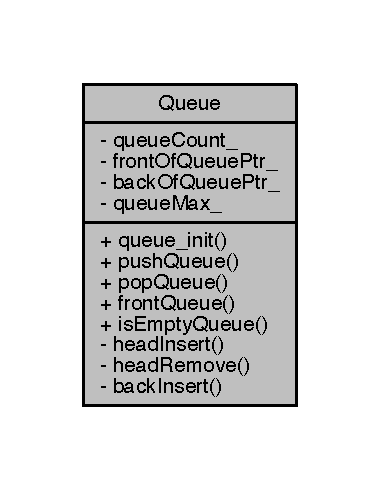
\includegraphics[width=182pt]{d9/d28/class_queue__coll__graph}
\end{center}
\end{figure}
\subsubsection*{Offentlige metoder}
\begin{DoxyCompactItemize}
\item 
void \hyperlink{class_queue_a4e0a3758d721506e7729f4d074a280ff}{queue\+\_\+init} (uint8 queue\+Max\+Size)
\begin{DoxyCompactList}\small\item\em Initialiser \hyperlink{class_queue}{Queue} modulet. \end{DoxyCompactList}\item 
void \hyperlink{class_queue_a0012fa831aa1529e5ed3a6610b733423}{push\+Queue} (const struct \hyperlink{queue_8h_df/d8c/struct_action}{Action} data)
\begin{DoxyCompactList}\small\item\em Indsætter et element i køen. \end{DoxyCompactList}\item 
void \hyperlink{class_queue_a9ecab9ecdedfc331aed9a0ae63ce193b}{pop\+Queue} ()
\begin{DoxyCompactList}\small\item\em Fjerner et element i køen. \end{DoxyCompactList}\item 
struct \hyperlink{queue_8h_df/d8c/struct_action}{Action} \hyperlink{class_queue_a49c50ba30a42033068d8d8e6a23c6ca1}{front\+Queue} ()
\begin{DoxyCompactList}\small\item\em Viser et element fra køen. \end{DoxyCompactList}\item 
uint8 \hyperlink{class_queue_aafb324c79731abdc228dbf94d86722a3}{is\+Empty\+Queue} ()
\begin{DoxyCompactList}\small\item\em Retuner status af køen. \end{DoxyCompactList}\end{DoxyCompactItemize}
\subsubsection*{Private metoder}
\begin{DoxyCompactItemize}
\item 
void \hyperlink{class_queue_a1189c09234d75518492525645a05db07}{head\+Insert} (struct \hyperlink{queue_8c_db/d8b/struct_node}{Node} $\ast$$\ast$head\+Ptr, const struct \hyperlink{queue_8h_df/d8c/struct_action}{Action} data)
\begin{DoxyCompactList}\small\item\em Indsætter forreste i listen. \end{DoxyCompactList}\item 
void \hyperlink{class_queue_ae54666c891fd21d5497f48c385a00b74}{head\+Remove} (struct \hyperlink{queue_8c_db/d8b/struct_node}{Node} $\ast$$\ast$head\+Ptr)
\begin{DoxyCompactList}\small\item\em Fjerner fra listen. \end{DoxyCompactList}\item 
void \hyperlink{class_queue_a5a25a737ba7dff74923f5cb04e19164c}{back\+Insert} (struct \hyperlink{queue_8c_db/d8b/struct_node}{Node} $\ast$$\ast$back\+Ptr, const struct \hyperlink{queue_8h_df/d8c/struct_action}{Action} data)
\begin{DoxyCompactList}\small\item\em Indsætter bagerst i listen. \end{DoxyCompactList}\end{DoxyCompactItemize}
\subsubsection*{Statiske, private attributter}
\begin{DoxyCompactItemize}
\item 
static struct \hyperlink{queue_8c_db/d8b/struct_node}{Node} $\ast$ \hyperlink{class_queue_aa48f05218d0a78402821c8aa9bdad06a}{front\+Of\+Queue\+Ptr\+\_\+}
\begin{DoxyCompactList}\small\item\em Pointer til foreste element i køen. \end{DoxyCompactList}\item 
static struct \hyperlink{queue_8c_db/d8b/struct_node}{Node} $\ast$ \hyperlink{class_queue_a225d2c9ad4e83d6da443e99b8869a51c}{back\+Of\+Queue\+Ptr\+\_\+}
\begin{DoxyCompactList}\small\item\em Pointer til bagerste element i køen. \end{DoxyCompactList}\item 
static uint8 \hyperlink{class_queue_acb6b6e88c9e4d12839594b31e6ff7c5a}{queue\+Max\+\_\+}
\begin{DoxyCompactList}\small\item\em Køens max. \end{DoxyCompactList}\item 
static uint8 \hyperlink{class_queue_ad260f9ccca00e80d161bbf3e70c3ffa6}{queue\+Count\+\_\+}
\begin{DoxyCompactList}\small\item\em Kø element tæller. \end{DoxyCompactList}\end{DoxyCompactItemize}


\subsubsection{Detaljeret beskrivelse}
\hyperlink{class_queue}{Queue} class. 

En F\+I\+FO kø der er opbygget af en single linket liste. \begin{DoxyAuthor}{Forfatter}
Jeppe Stærk Antonsen (\href{mailto:201271201@uni.au.dk}{\tt 201271201@uni.\+au.\+dk}) 
\end{DoxyAuthor}


\subsubsection{Dokumentation af medlemsfunktioner}
\index{Queue@{Queue}!back\+Insert@{back\+Insert}}
\index{back\+Insert@{back\+Insert}!Queue@{Queue}}
\paragraph[{\texorpdfstring{back\+Insert(struct Node $\ast$$\ast$back\+Ptr, const struct Action data)}{backInsert(struct Node **backPtr, const struct Action data)}}]{\setlength{\rightskip}{0pt plus 5cm}void back\+Insert (
\begin{DoxyParamCaption}
\item[{struct {\bf Node} $\ast$$\ast$}]{back\+Ptr, }
\item[{const struct {\bf Action}}]{data}
\end{DoxyParamCaption}
)\hspace{0.3cm}{\ttfamily [private]}}\hypertarget{class_queue_a5a25a737ba7dff74923f5cb04e19164c}{}\label{class_queue_a5a25a737ba7dff74923f5cb04e19164c}


Indsætter bagerst i listen. 

Indsætter det angivet element bagerst i den underlægende linked liste. 
\begin{DoxyParams}[1]{Parametre}
\mbox{\tt in}  & {\em back\+Ptr} & Pointer til det bagerste element i listen. \\
\hline
\mbox{\tt in}  & {\em data} & \hyperlink{class_data}{Data} der skal indsættes i listen.\\
\hline
\end{DoxyParams}
\begin{DoxyAuthor}{Forfatter}
Jeppe Stærk Antonsen (\href{mailto:201271201@uni.au.dk}{\tt 201271201@uni.\+au.\+dk}) 
\end{DoxyAuthor}


Defineret på linje 248 i filen queue.\+c.



Indeholder referencer til Node\+::data\+\_\+ og Node\+::next\+\_\+.


\begin{DoxyCode}
249 \{
250   \textcolor{keywordflow}{if}(*backPtr == NULL)
251   \{
252     \textcolor{keywordflow}{return};
253   \}
254   
255   \textcolor{keyword}{struct }\hyperlink{queue_8c_db/d8b/struct_node}{Node}* next = (*backPtr)->\hyperlink{queue_8c_a882bca6dea645e11ca1df6bc3c30ac42}{next\_};
256   \textcolor{keyword}{struct }\hyperlink{queue_8c_db/d8b/struct_node}{Node}* temp = (\textcolor{keyword}{struct }\hyperlink{queue_8c_db/d8b/struct_node}{Node}*)malloc(\textcolor{keyword}{sizeof}(\textcolor{keyword}{struct} \hyperlink{queue_8c_db/d8b/struct_node}{Node}));
257   temp->\hyperlink{queue_8c_ab134027ce40d71eaa8746f6a8e7d4b8a}{data\_} = data;
258   temp->\hyperlink{queue_8c_a882bca6dea645e11ca1df6bc3c30ac42}{next\_} = next;
259   (*backPtr)->\hyperlink{queue_8c_a882bca6dea645e11ca1df6bc3c30ac42}{next\_} = temp;
260 \}
\end{DoxyCode}
\index{Queue@{Queue}!front\+Queue@{front\+Queue}}
\index{front\+Queue@{front\+Queue}!Queue@{Queue}}
\paragraph[{\texorpdfstring{front\+Queue()}{frontQueue()}}]{\setlength{\rightskip}{0pt plus 5cm}struct {\bf Action} front\+Queue (
\begin{DoxyParamCaption}
\item[{void}]{}
\end{DoxyParamCaption}
)}\hypertarget{class_queue_a49c50ba30a42033068d8d8e6a23c6ca1}{}\label{class_queue_a49c50ba30a42033068d8d8e6a23c6ca1}


Viser et element fra køen. 

Viser det foreste element i F\+I\+FO køen.

\begin{DoxyAuthor}{Forfatter}
Jeppe Stærk Antonsen (\href{mailto:201271201@uni.au.dk}{\tt 201271201@uni.\+au.\+dk}) 
\end{DoxyAuthor}


Defineret på linje 170 i filen queue.\+c.



Indeholder referencer til Node\+::data\+\_\+.



Refereret til af main().


\begin{DoxyCode}
171 \{
172   DEBUG\_PutString(\textcolor{stringliteral}{"Q=: count: "});
173   DEBUG\_PutHexByte(\hyperlink{class_queue_ad260f9ccca00e80d161bbf3e70c3ffa6}{queueCount\_});
174   DEBUG\_PutCRLF();
175   \textcolor{keywordflow}{return} \hyperlink{class_queue_aa48f05218d0a78402821c8aa9bdad06a}{frontOfQueuePtr\_}->\hyperlink{queue_8c_ab134027ce40d71eaa8746f6a8e7d4b8a}{data\_};
176 \}
\end{DoxyCode}


Her er kalder-\/grafen for denne funktion\+:
\nopagebreak
\begin{figure}[H]
\begin{center}
\leavevmode
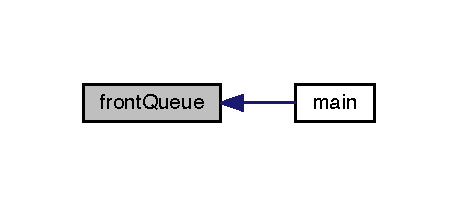
\includegraphics[width=220pt]{d4/da4/class_queue_a49c50ba30a42033068d8d8e6a23c6ca1_icgraph}
\end{center}
\end{figure}


\index{Queue@{Queue}!head\+Insert@{head\+Insert}}
\index{head\+Insert@{head\+Insert}!Queue@{Queue}}
\paragraph[{\texorpdfstring{head\+Insert(struct Node $\ast$$\ast$head\+Ptr, const struct Action data)}{headInsert(struct Node **headPtr, const struct Action data)}}]{\setlength{\rightskip}{0pt plus 5cm}void head\+Insert (
\begin{DoxyParamCaption}
\item[{struct {\bf Node} $\ast$$\ast$}]{head\+Ptr, }
\item[{const struct {\bf Action}}]{data}
\end{DoxyParamCaption}
)\hspace{0.3cm}{\ttfamily [private]}}\hypertarget{class_queue_a1189c09234d75518492525645a05db07}{}\label{class_queue_a1189c09234d75518492525645a05db07}


Indsætter forreste i listen. 

Indsætter det angivet element forreste i den underlægende linked liste. 
\begin{DoxyParams}[1]{Parametre}
\mbox{\tt in}  & {\em head\+Ptr} & Pointer til det foreste element i listen. \\
\hline
\mbox{\tt in}  & {\em data} & \hyperlink{class_data}{Data} der skal indsættes i listen.\\
\hline
\end{DoxyParams}
\begin{DoxyAuthor}{Forfatter}
Jeppe Stærk Antonsen (\href{mailto:201271201@uni.au.dk}{\tt 201271201@uni.\+au.\+dk}) 
\end{DoxyAuthor}


Defineret på linje 206 i filen queue.\+c.



Indeholder referencer til Node\+::data\+\_\+ og Node\+::next\+\_\+.


\begin{DoxyCode}
207 \{
208   \textcolor{keyword}{struct }\hyperlink{queue_8c_db/d8b/struct_node}{Node}* temp = (\textcolor{keyword}{struct }\hyperlink{queue_8c_db/d8b/struct_node}{Node}*)malloc(\textcolor{keyword}{sizeof}(\textcolor{keyword}{struct} \hyperlink{queue_8c_db/d8b/struct_node}{Node}));
209   \textcolor{keywordflow}{if}(temp == NULL)
210   \{
211     \textcolor{keywordflow}{return};
212   \}
213   
214   temp->\hyperlink{queue_8c_ab134027ce40d71eaa8746f6a8e7d4b8a}{data\_} = data;
215   temp->\hyperlink{queue_8c_a882bca6dea645e11ca1df6bc3c30ac42}{next\_} = NULL;
216   
217   *headPtr = temp;
218 \}
\end{DoxyCode}
\index{Queue@{Queue}!head\+Remove@{head\+Remove}}
\index{head\+Remove@{head\+Remove}!Queue@{Queue}}
\paragraph[{\texorpdfstring{head\+Remove(struct Node $\ast$$\ast$head\+Ptr)}{headRemove(struct Node **headPtr)}}]{\setlength{\rightskip}{0pt plus 5cm}void head\+Remove (
\begin{DoxyParamCaption}
\item[{struct {\bf Node} $\ast$$\ast$}]{head\+Ptr}
\end{DoxyParamCaption}
)\hspace{0.3cm}{\ttfamily [private]}}\hypertarget{class_queue_ae54666c891fd21d5497f48c385a00b74}{}\label{class_queue_ae54666c891fd21d5497f48c385a00b74}


Fjerner fra listen. 

Fjerner det forreste element i den underlæggende linked liste 
\begin{DoxyParams}[1]{Parametre}
\mbox{\tt in}  & {\em head\+Ptr} & Pointer til det forreste element i listen.\\
\hline
\end{DoxyParams}
\begin{DoxyAuthor}{Forfatter}
Jeppe Stærk Antonsen (\href{mailto:201271201@uni.au.dk}{\tt 201271201@uni.\+au.\+dk}) 
\end{DoxyAuthor}


Defineret på linje 228 i filen queue.\+c.



Indeholder referencer til Node\+::next\+\_\+.


\begin{DoxyCode}
229 \{
230   \textcolor{keywordflow}{if}(headPtr != NULL)
231   \{
232     \textcolor{keyword}{struct }\hyperlink{queue_8c_db/d8b/struct_node}{Node}* condemned;
233     condemned = *headPtr;
234     *headPtr = (*headPtr)->\hyperlink{queue_8c_a882bca6dea645e11ca1df6bc3c30ac42}{next\_};
235     free(condemned);
236   \}
237 \}
\end{DoxyCode}
\index{Queue@{Queue}!is\+Empty\+Queue@{is\+Empty\+Queue}}
\index{is\+Empty\+Queue@{is\+Empty\+Queue}!Queue@{Queue}}
\paragraph[{\texorpdfstring{is\+Empty\+Queue()}{isEmptyQueue()}}]{\setlength{\rightskip}{0pt plus 5cm}uint8 is\+Empty\+Queue (
\begin{DoxyParamCaption}
\item[{void}]{}
\end{DoxyParamCaption}
)}\hypertarget{class_queue_aafb324c79731abdc228dbf94d86722a3}{}\label{class_queue_aafb324c79731abdc228dbf94d86722a3}


Retuner status af køen. 

Kontrollere om køen er tom.

\begin{DoxyAuthor}{Forfatter}
Jeppe Stærk Antonsen (\href{mailto:201271201@uni.au.dk}{\tt 201271201@uni.\+au.\+dk}) 
\end{DoxyAuthor}


Defineret på linje 185 i filen queue.\+c.



Refereret til af main().


\begin{DoxyCode}
186 \{
187   \textcolor{keywordflow}{if}(\hyperlink{class_queue_aa48f05218d0a78402821c8aa9bdad06a}{frontOfQueuePtr\_} == NULL)
188   \{
189     \textcolor{keywordflow}{return} 1;
190   \}
191   \textcolor{keywordflow}{else}
192   \{
193     \textcolor{keywordflow}{return} 0;
194   \}
195 \}
\end{DoxyCode}


Her er kalder-\/grafen for denne funktion\+:
\nopagebreak
\begin{figure}[H]
\begin{center}
\leavevmode
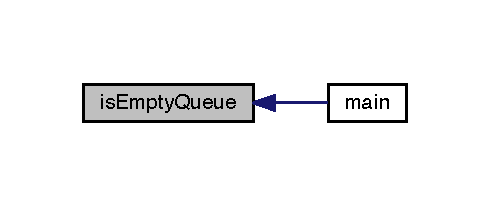
\includegraphics[width=235pt]{d4/da4/class_queue_aafb324c79731abdc228dbf94d86722a3_icgraph}
\end{center}
\end{figure}


\index{Queue@{Queue}!pop\+Queue@{pop\+Queue}}
\index{pop\+Queue@{pop\+Queue}!Queue@{Queue}}
\paragraph[{\texorpdfstring{pop\+Queue()}{popQueue()}}]{\setlength{\rightskip}{0pt plus 5cm}void pop\+Queue (
\begin{DoxyParamCaption}
\item[{void}]{}
\end{DoxyParamCaption}
)}\hypertarget{class_queue_a9ecab9ecdedfc331aed9a0ae63ce193b}{}\label{class_queue_a9ecab9ecdedfc331aed9a0ae63ce193b}


Fjerner et element i køen. 

Fjerner det foreste element i F\+I\+FO køen.

\begin{DoxyAuthor}{Forfatter}
Jeppe Stærk Antonsen (\href{mailto:201271201@uni.au.dk}{\tt 201271201@uni.\+au.\+dk}) 
\end{DoxyAuthor}


Defineret på linje 149 i filen queue.\+c.



Indeholder referencer til head\+Remove() og is\+Empty\+Queue().



Refereret til af main().


\begin{DoxyCode}
150 \{
151   \hyperlink{class_queue_ae54666c891fd21d5497f48c385a00b74}{headRemove}(&\hyperlink{class_queue_aa48f05218d0a78402821c8aa9bdad06a}{frontOfQueuePtr\_});
152   \hyperlink{class_queue_ad260f9ccca00e80d161bbf3e70c3ffa6}{queueCount\_}--;
153   \textcolor{keywordflow}{if}(\hyperlink{class_queue_aafb324c79731abdc228dbf94d86722a3}{isEmptyQueue}() == 1)
154   \{
155     \hyperlink{class_queue_a225d2c9ad4e83d6da443e99b8869a51c}{backOfQueuePtr\_} = NULL;
156   \}
157   DEBUG\_PutString(\textcolor{stringliteral}{"-Q: count: "});
158   DEBUG\_PutHexByte(\hyperlink{class_queue_ad260f9ccca00e80d161bbf3e70c3ffa6}{queueCount\_});
159   DEBUG\_PutCRLF();
160   DEBUG\_PutCRLF();
161 \}
\end{DoxyCode}


Her er kald-\/grafen for denne funktion\+:
\nopagebreak
\begin{figure}[H]
\begin{center}
\leavevmode
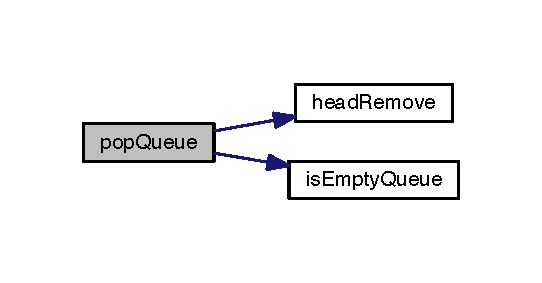
\includegraphics[width=260pt]{d4/da4/class_queue_a9ecab9ecdedfc331aed9a0ae63ce193b_cgraph}
\end{center}
\end{figure}




Her er kalder-\/grafen for denne funktion\+:
\nopagebreak
\begin{figure}[H]
\begin{center}
\leavevmode
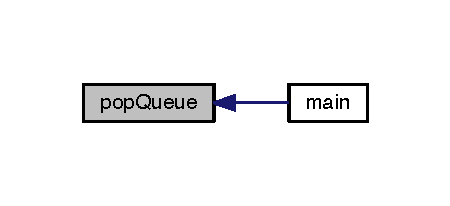
\includegraphics[width=216pt]{d4/da4/class_queue_a9ecab9ecdedfc331aed9a0ae63ce193b_icgraph}
\end{center}
\end{figure}


\index{Queue@{Queue}!push\+Queue@{push\+Queue}}
\index{push\+Queue@{push\+Queue}!Queue@{Queue}}
\paragraph[{\texorpdfstring{push\+Queue(const struct Action data)}{pushQueue(const struct Action data)}}]{\setlength{\rightskip}{0pt plus 5cm}void push\+Queue (
\begin{DoxyParamCaption}
\item[{const struct {\bf Action}}]{data}
\end{DoxyParamCaption}
)}\hypertarget{class_queue_a0012fa831aa1529e5ed3a6610b733423}{}\label{class_queue_a0012fa831aa1529e5ed3a6610b733423}


Indsætter et element i køen. 

Indsætter det angivet element bagerst i F\+I\+FO køen. 
\begin{DoxyParams}[1]{Parametre}
\mbox{\tt in}  & {\em data} & \hyperlink{class_data}{Data} der skal indsættes i køen.\\
\hline
\end{DoxyParams}
\begin{DoxyAuthor}{Forfatter}
Jeppe Stærk Antonsen (\href{mailto:201271201@uni.au.dk}{\tt 201271201@uni.\+au.\+dk}) 
\end{DoxyAuthor}


Defineret på linje 107 i filen queue.\+c.



Indeholder referencer til back\+Insert(), Action\+::cmd, head\+Insert(), is\+Empty\+Queue(), Node\+::next\+\_\+ og Action\+::val.



Refereret til af I2\+C\+::\+I2\+C\+S\+\_\+\+I2\+C\+\_\+\+I\+S\+R\+\_\+\+Exit\+Callback().


\begin{DoxyCode}
108 \{
109   \textcolor{keywordflow}{if}(\hyperlink{class_queue_ad260f9ccca00e80d161bbf3e70c3ffa6}{queueCount\_}<\hyperlink{class_queue_acb6b6e88c9e4d12839594b31e6ff7c5a}{queueMax\_})
110   \{
111     \textcolor{keywordflow}{if}(\hyperlink{class_queue_aafb324c79731abdc228dbf94d86722a3}{isEmptyQueue}() != 1)
112     \{
113       \hyperlink{class_queue_a5a25a737ba7dff74923f5cb04e19164c}{backInsert}(&\hyperlink{class_queue_a225d2c9ad4e83d6da443e99b8869a51c}{backOfQueuePtr\_}, data);
114       \hyperlink{class_queue_a225d2c9ad4e83d6da443e99b8869a51c}{backOfQueuePtr\_} = \hyperlink{class_queue_a225d2c9ad4e83d6da443e99b8869a51c}{backOfQueuePtr\_}->\hyperlink{queue_8c_a882bca6dea645e11ca1df6bc3c30ac42}{next\_};
115       \hyperlink{class_queue_ad260f9ccca00e80d161bbf3e70c3ffa6}{queueCount\_}++;
116     \}
117     \textcolor{keywordflow}{else}
118     \{
119       \hyperlink{class_queue_a1189c09234d75518492525645a05db07}{headInsert}(&\hyperlink{class_queue_aa48f05218d0a78402821c8aa9bdad06a}{frontOfQueuePtr\_}, data);
120       \hyperlink{class_queue_a225d2c9ad4e83d6da443e99b8869a51c}{backOfQueuePtr\_} = \hyperlink{class_queue_aa48f05218d0a78402821c8aa9bdad06a}{frontOfQueuePtr\_};
121       \hyperlink{class_queue_ad260f9ccca00e80d161bbf3e70c3ffa6}{queueCount\_}++;
122     \}
123     DEBUG\_PutString(\textcolor{stringliteral}{"Q+: count: "});
124     DEBUG\_PutHexByte(\hyperlink{class_queue_ad260f9ccca00e80d161bbf3e70c3ffa6}{queueCount\_});
125     DEBUG\_PutString(\textcolor{stringliteral}{" cmd: "});
126     DEBUG\_PutHexByte(data.\hyperlink{queue_8h_a85092d82ab6ea85dad51ba78cbda36a0}{cmd});
127     DEBUG\_PutString(\textcolor{stringliteral}{" val: "});
128     DEBUG\_PutHexByte(data.\hyperlink{queue_8h_aa0ccb5ee6d882ee3605ff47745c6467b}{val});
129     DEBUG\_PutCRLF();
130     DEBUG\_PutCRLF();
131   \}
132   \textcolor{keywordflow}{else}
133   \{
134     DEBUG\_PutString(\textcolor{stringliteral}{"Q~: ERROR! Queue FULL!!! count: "});
135     DEBUG\_PutHexByte(\hyperlink{class_queue_ad260f9ccca00e80d161bbf3e70c3ffa6}{queueCount\_});
136     DEBUG\_PutCRLF();
137     DEBUG\_PutCRLF();
138   \}
139   
140 \}
\end{DoxyCode}


Her er kald-\/grafen for denne funktion\+:
\nopagebreak
\begin{figure}[H]
\begin{center}
\leavevmode
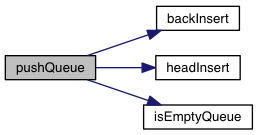
\includegraphics[width=265pt]{d4/da4/class_queue_a0012fa831aa1529e5ed3a6610b733423_cgraph}
\end{center}
\end{figure}




Her er kalder-\/grafen for denne funktion\+:
\nopagebreak
\begin{figure}[H]
\begin{center}
\leavevmode
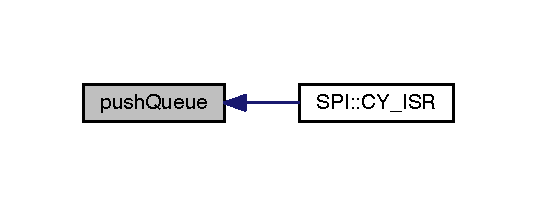
\includegraphics[width=347pt]{d4/da4/class_queue_a0012fa831aa1529e5ed3a6610b733423_icgraph}
\end{center}
\end{figure}


\index{Queue@{Queue}!queue\+\_\+init@{queue\+\_\+init}}
\index{queue\+\_\+init@{queue\+\_\+init}!Queue@{Queue}}
\paragraph[{\texorpdfstring{queue\+\_\+init(uint8 queue\+Max\+Size)}{queue_init(uint8 queueMaxSize)}}]{\setlength{\rightskip}{0pt plus 5cm}void queue\+\_\+init (
\begin{DoxyParamCaption}
\item[{uint8}]{queue\+Max\+Size}
\end{DoxyParamCaption}
)}\hypertarget{class_queue_a4e0a3758d721506e7729f4d074a280ff}{}\label{class_queue_a4e0a3758d721506e7729f4d074a280ff}


Initialiser \hyperlink{class_queue}{Queue} modulet. 

Initailiser køen med den ønsket max størelse.

\begin{DoxyAuthor}{Forfatter}
Jeppe Stærk Antonsen (\href{mailto:201271201@uni.au.dk}{\tt 201271201@uni.\+au.\+dk}) 
\end{DoxyAuthor}


Defineret på linje 89 i filen queue.\+c.



Indeholder referencer til Node\+::next\+\_\+.



Refereret til af main().


\begin{DoxyCode}
90 \{
91   \hyperlink{class_queue_aa48f05218d0a78402821c8aa9bdad06a}{frontOfQueuePtr\_} = NULL;
92   \hyperlink{class_queue_aa48f05218d0a78402821c8aa9bdad06a}{frontOfQueuePtr\_}->\hyperlink{queue_8c_a882bca6dea645e11ca1df6bc3c30ac42}{next\_} = NULL;
93   \hyperlink{class_queue_a225d2c9ad4e83d6da443e99b8869a51c}{backOfQueuePtr\_} = NULL;
94   \hyperlink{class_queue_a225d2c9ad4e83d6da443e99b8869a51c}{backOfQueuePtr\_}->\hyperlink{queue_8c_a882bca6dea645e11ca1df6bc3c30ac42}{next\_} = NULL;
95   \hyperlink{class_queue_acb6b6e88c9e4d12839594b31e6ff7c5a}{queueMax\_} = queueMaxSize;
96   \hyperlink{class_queue_ad260f9ccca00e80d161bbf3e70c3ffa6}{queueCount\_} = 0;
97 \}
\end{DoxyCode}


Her er kalder-\/grafen for denne funktion\+:
\nopagebreak
\begin{figure}[H]
\begin{center}
\leavevmode
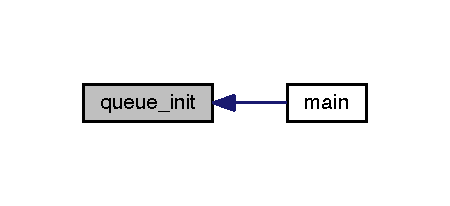
\includegraphics[width=216pt]{d4/da4/class_queue_a4e0a3758d721506e7729f4d074a280ff_icgraph}
\end{center}
\end{figure}




\subsubsection{Felt-\/dokumentation}
\index{Queue@{Queue}!back\+Of\+Queue\+Ptr\+\_\+@{back\+Of\+Queue\+Ptr\+\_\+}}
\index{back\+Of\+Queue\+Ptr\+\_\+@{back\+Of\+Queue\+Ptr\+\_\+}!Queue@{Queue}}
\paragraph[{\texorpdfstring{back\+Of\+Queue\+Ptr\+\_\+}{backOfQueuePtr_}}]{\setlength{\rightskip}{0pt plus 5cm}struct {\bf Node}$\ast$ back\+Of\+Queue\+Ptr\+\_\+\hspace{0.3cm}{\ttfamily [static]}, {\ttfamily [private]}}\hypertarget{class_queue_a225d2c9ad4e83d6da443e99b8869a51c}{}\label{class_queue_a225d2c9ad4e83d6da443e99b8869a51c}


Pointer til bagerste element i køen. 

En \hyperlink{queue_8c_db/d8b/struct_node}{Node} pointer der indeholder adressen på det bagerste elementet i køen.

\begin{DoxyAuthor}{Forfatter}
Jeppe Stærk Antonsen (\href{mailto:201271201@uni.au.dk}{\tt 201271201@uni.\+au.\+dk}) 
\end{DoxyAuthor}


Defineret på linje 48 i filen queue.\+c.

\index{Queue@{Queue}!front\+Of\+Queue\+Ptr\+\_\+@{front\+Of\+Queue\+Ptr\+\_\+}}
\index{front\+Of\+Queue\+Ptr\+\_\+@{front\+Of\+Queue\+Ptr\+\_\+}!Queue@{Queue}}
\paragraph[{\texorpdfstring{front\+Of\+Queue\+Ptr\+\_\+}{frontOfQueuePtr_}}]{\setlength{\rightskip}{0pt plus 5cm}struct {\bf Node}$\ast$ front\+Of\+Queue\+Ptr\+\_\+\hspace{0.3cm}{\ttfamily [static]}, {\ttfamily [private]}}\hypertarget{class_queue_aa48f05218d0a78402821c8aa9bdad06a}{}\label{class_queue_aa48f05218d0a78402821c8aa9bdad06a}


Pointer til foreste element i køen. 

En \hyperlink{queue_8c_db/d8b/struct_node}{Node} pointer der indeholder adressen på det foreste elementet i køen.

\begin{DoxyAuthor}{Forfatter}
Jeppe Stærk Antonsen (\href{mailto:201271201@uni.au.dk}{\tt 201271201@uni.\+au.\+dk}) 
\end{DoxyAuthor}


Defineret på linje 39 i filen queue.\+c.

\index{Queue@{Queue}!queue\+Count\+\_\+@{queue\+Count\+\_\+}}
\index{queue\+Count\+\_\+@{queue\+Count\+\_\+}!Queue@{Queue}}
\paragraph[{\texorpdfstring{queue\+Count\+\_\+}{queueCount_}}]{\setlength{\rightskip}{0pt plus 5cm}uint8 queue\+Count\+\_\+\hspace{0.3cm}{\ttfamily [static]}, {\ttfamily [private]}}\hypertarget{class_queue_ad260f9ccca00e80d161bbf3e70c3ffa6}{}\label{class_queue_ad260f9ccca00e80d161bbf3e70c3ffa6}


Kø element tæller. 

Bruges til at tælle hvor mange elementer der er i køen.

\begin{DoxyAuthor}{Forfatter}
Jeppe Stærk Antonsen (\href{mailto:201271201@uni.au.dk}{\tt 201271201@uni.\+au.\+dk}) 
\end{DoxyAuthor}


Defineret på linje 66 i filen queue.\+c.

\index{Queue@{Queue}!queue\+Max\+\_\+@{queue\+Max\+\_\+}}
\index{queue\+Max\+\_\+@{queue\+Max\+\_\+}!Queue@{Queue}}
\paragraph[{\texorpdfstring{queue\+Max\+\_\+}{queueMax_}}]{\setlength{\rightskip}{0pt plus 5cm}uint8 queue\+Max\+\_\+\hspace{0.3cm}{\ttfamily [static]}, {\ttfamily [private]}}\hypertarget{class_queue_acb6b6e88c9e4d12839594b31e6ff7c5a}{}\label{class_queue_acb6b6e88c9e4d12839594b31e6ff7c5a}


Køens max. 

Laver ved initialisering der ønsket antal for max elementer i køen

\begin{DoxyAuthor}{Forfatter}
Jeppe Stærk Antonsen (\href{mailto:201271201@uni.au.dk}{\tt 201271201@uni.\+au.\+dk}) 
\end{DoxyAuthor}


Defineret på linje 57 i filen queue.\+c.



Dokumentationen for denne klasse blev genereret ud fra filerne\+:\begin{DoxyCompactItemize}
\item 
\hyperlink{queue_8h}{queue.\+h}\item 
\hyperlink{queue_8c}{queue.\+c}\end{DoxyCompactItemize}

\hypertarget{class_sensor_data}{}\subsection{Sensor\+Data Klasse-\/reference}
\label{class_sensor_data}\index{Sensor\+Data@{Sensor\+Data}}


Container for sensor data.  




{\ttfamily \#include $<$Sensor\+Data.\+h$>$}



Samarbejdsdiagram for Sensor\+Data\+:
\nopagebreak
\begin{figure}[H]
\begin{center}
\leavevmode
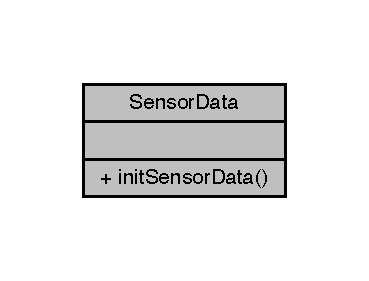
\includegraphics[width=177pt]{dc/d1d/class_sensor_data__coll__graph}
\end{center}
\end{figure}
\subsubsection*{Offentlige metoder}
\begin{DoxyCompactItemize}
\item 
void \hyperlink{class_sensor_data_ad900f3738890946c3d0516ddd9105474}{init\+Sensor\+Data} ()
\begin{DoxyCompactList}\small\item\em Initializes the \hyperlink{class_sensor_data}{Sensor\+Data} struct parts that need initial values. \end{DoxyCompactList}\end{DoxyCompactItemize}


\subsubsection{Detaljeret beskrivelse}
Container for sensor data. 

\begin{DoxyAuthor}{Forfatter}
Simon Nejmann (\href{mailto:19981127@uni.au.dk}{\tt 19981127@uni.\+au.\+dk}) 
\end{DoxyAuthor}


\subsubsection{Dokumentation af medlemsfunktioner}
\index{Sensor\+Data@{Sensor\+Data}!init\+Sensor\+Data@{init\+Sensor\+Data}}
\index{init\+Sensor\+Data@{init\+Sensor\+Data}!Sensor\+Data@{Sensor\+Data}}
\paragraph[{\texorpdfstring{init\+Sensor\+Data()}{initSensorData()}}]{\setlength{\rightskip}{0pt plus 5cm}void init\+Sensor\+Data (
\begin{DoxyParamCaption}
{}
\end{DoxyParamCaption}
)}\hypertarget{class_sensor_data_ad900f3738890946c3d0516ddd9105474}{}\label{class_sensor_data_ad900f3738890946c3d0516ddd9105474}


Initializes the \hyperlink{class_sensor_data}{Sensor\+Data} struct parts that need initial values. 

Debug define. Comment out to suppress debug prints

\begin{DoxyAuthor}{Forfatter}
Simon Nejmann (\href{mailto:19981127@uni.au.dk}{\tt 19981127@uni.\+au.\+dk})

Simon Nejmann (\href{mailto:19981127@uni.au.dk}{\tt 19981127@uni.\+au.\+dk}) 
\end{DoxyAuthor}


Defineret på linje 17 i filen Sensor\+Data.\+c.



Indeholder referencer til sensor\+Data\+T\+::blue\+P\+W\+M\+Pct, sensor\+Data\+T\+::desired\+Lux, sensor\+Data\+T\+::desired\+Time\+Distance, sensor\+Data\+T\+::green\+P\+W\+M\+Pct, init\+Circular\+Mean(), sensor\+Data\+T\+::led\+Power, sensor\+Data\+T\+::\+Lumen\+Mean, sensor\+Data\+T\+::movement\+Alert\+On, sensor\+Data\+T\+::red\+P\+W\+M\+Pct og sensor\+Data.



Refereret til af main().


\begin{DoxyCode}
18 \{
19     \hyperlink{_sensor_data_8h_a166db779eaca1ca69d6d63aa4fc36674}{sensorData}.\hyperlink{_sensor_data_8h_ad85f2cca5ef7520f1dc87fc48fc6d8e6}{desiredLux} = 0;
20     \hyperlink{_sensor_data_8h_a166db779eaca1ca69d6d63aa4fc36674}{sensorData}.\hyperlink{_sensor_data_8h_a477d7465dc8c397bdb795593df890d8b}{desiredTimeDistance} = 580;
21 
22     \hyperlink{_sensor_data_8h_a166db779eaca1ca69d6d63aa4fc36674}{sensorData}.\hyperlink{_sensor_data_8h_a722c0f415211bda0d848dd8edac4f1fe}{movementAlertOn} = 0;
23     
24     \hyperlink{_sensor_data_8h_a166db779eaca1ca69d6d63aa4fc36674}{sensorData}.\hyperlink{_sensor_data_8h_a3fc7bb7b6b9d39b2a6ae384d15fc5b9d}{ledPower} = 0;
25     \hyperlink{_sensor_data_8h_a166db779eaca1ca69d6d63aa4fc36674}{sensorData}.\hyperlink{_sensor_data_8h_a6ac22d5f267938f95b2261ffa3d5e2d2}{redPWMPct} = 255;
26     \hyperlink{_sensor_data_8h_a166db779eaca1ca69d6d63aa4fc36674}{sensorData}.\hyperlink{_sensor_data_8h_ac83b8257127d55e998596d703ff141ac}{greenPWMPct} = 255;
27     \hyperlink{_sensor_data_8h_a166db779eaca1ca69d6d63aa4fc36674}{sensorData}.\hyperlink{_sensor_data_8h_ac79167c0eef257a67503f9fbce9d377c}{bluePWMPct} = 255;
28 
29 \textcolor{preprocessor}{#ifdef DEBUG\_ON}
30     \hyperlink{_sensor_data_8h_a166db779eaca1ca69d6d63aa4fc36674}{sensorData}.\hyperlink{_sensor_data_8h_ad85f2cca5ef7520f1dc87fc48fc6d8e6}{desiredLux} = 0;
31     \hyperlink{_sensor_data_8h_a166db779eaca1ca69d6d63aa4fc36674}{sensorData}.\hyperlink{_sensor_data_8h_a722c0f415211bda0d848dd8edac4f1fe}{movementAlertOn} = 1;
32     \hyperlink{_sensor_data_8h_a166db779eaca1ca69d6d63aa4fc36674}{sensorData}.\hyperlink{_sensor_data_8h_a3fc7bb7b6b9d39b2a6ae384d15fc5b9d}{ledPower} = 1;
33 \textcolor{preprocessor}{#endif}
34     
35     \hyperlink{_circular_mean_8c_a5118b6b2a8751d4400b4ea2a0a15329a}{initCircularMean}(&\hyperlink{_sensor_data_8h_a166db779eaca1ca69d6d63aa4fc36674}{sensorData}.\hyperlink{_sensor_data_8h_a2ff5a38714ef318f86285c7d8fe4c8ea}{LumenMean});
36 \}
\end{DoxyCode}


Her er kald-\/grafen for denne funktion\+:
\nopagebreak
\begin{figure}[H]
\begin{center}
\leavevmode
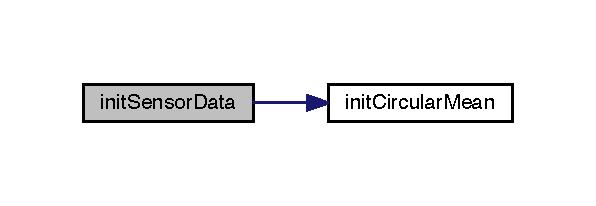
\includegraphics[width=286pt]{d2/d7e/class_sensor_data_ad900f3738890946c3d0516ddd9105474_cgraph}
\end{center}
\end{figure}




Her er kalder-\/grafen for denne funktion\+:
\nopagebreak
\begin{figure}[H]
\begin{center}
\leavevmode
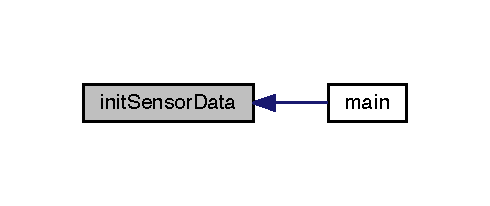
\includegraphics[width=235pt]{d2/d7e/class_sensor_data_ad900f3738890946c3d0516ddd9105474_icgraph}
\end{center}
\end{figure}




Dokumentationen for denne klasse blev genereret ud fra filerne\+:\begin{DoxyCompactItemize}
\item 
\hyperlink{_sensor_data_8h}{Sensor\+Data.\+h}\item 
\hyperlink{_sensor_data_8c}{Sensor\+Data.\+c}\end{DoxyCompactItemize}

\section{Fil-\/dokumentation}
\hypertarget{_circular_mean_8c}{}\subsection{Circular\+Mean.\+c filreference}
\label{_circular_mean_8c}\index{Circular\+Mean.\+c@{Circular\+Mean.\+c}}
{\ttfamily \#include \char`\"{}Circular\+Mean.\+h\char`\"{}}\\*
Inklusions-\/afhængighedsgraf for Circular\+Mean.\+c\+:
\nopagebreak
\begin{figure}[H]
\begin{center}
\leavevmode
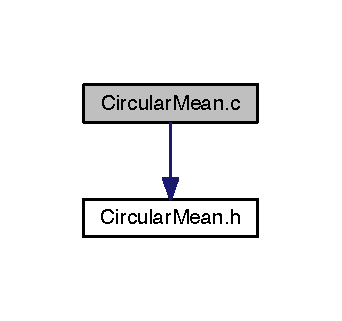
\includegraphics[width=164pt]{d2/da5/_circular_mean_8c__incl}
\end{center}
\end{figure}
\subsubsection*{Funktioner}
\begin{DoxyCompactItemize}
\item 
void \hyperlink{_circular_mean_8c_a5118b6b2a8751d4400b4ea2a0a15329a}{init\+Circular\+Mean} (struct \hyperlink{_circular_mean_8h_d2/ddd/struct_circular_mean}{Circular\+Mean} $\ast$buf)
\begin{DoxyCompactList}\small\item\em Initialize a \hyperlink{_circular_mean_8h_d2/ddd/struct_circular_mean}{Circular\+Mean} struct. \end{DoxyCompactList}\item 
void \hyperlink{_circular_mean_8c_a6dfc9bb6b16de641325dc73e7f31f7fc}{insert\+Value} (struct \hyperlink{_circular_mean_8h_d2/ddd/struct_circular_mean}{Circular\+Mean} $\ast$buf, int val)
\begin{DoxyCompactList}\small\item\em Insert value, possibly overwriting oldest entry. \end{DoxyCompactList}\item 
int \hyperlink{_circular_mean_8c_a521968471dd1466d7efc8deb9fb14118}{get\+Mean\+Value} (struct \hyperlink{_circular_mean_8h_d2/ddd/struct_circular_mean}{Circular\+Mean} $\ast$buf)
\begin{DoxyCompactList}\small\item\em Get the average value of all the ints in the buffer. \end{DoxyCompactList}\end{DoxyCompactItemize}


\subsubsection{Funktions-\/dokumentation}
\index{Circular\+Mean.\+c@{Circular\+Mean.\+c}!get\+Mean\+Value@{get\+Mean\+Value}}
\index{get\+Mean\+Value@{get\+Mean\+Value}!Circular\+Mean.\+c@{Circular\+Mean.\+c}}
\paragraph[{\texorpdfstring{get\+Mean\+Value(struct Circular\+Mean $\ast$buf)}{getMeanValue(struct CircularMean *buf)}}]{\setlength{\rightskip}{0pt plus 5cm}int get\+Mean\+Value (
\begin{DoxyParamCaption}
\item[{struct {\bf Circular\+Mean} $\ast$}]{buf}
\end{DoxyParamCaption}
)}\hypertarget{_circular_mean_8c_a521968471dd1466d7efc8deb9fb14118}{}\label{_circular_mean_8c_a521968471dd1466d7efc8deb9fb14118}


Get the average value of all the ints in the buffer. 


\begin{DoxyParams}[1]{Parametre}
\mbox{\tt in}  & {\em buf} & Pointer to the \hyperlink{_circular_mean_8h_d2/ddd/struct_circular_mean}{Circular\+Mean} \\
\hline
\end{DoxyParams}
\begin{DoxyReturn}{Returnerer}
The average value calculated
\end{DoxyReturn}
\begin{DoxyAuthor}{Forfatter}
Simon Nejmann (\href{mailto:19981127@uni.au.dk}{\tt 19981127@uni.\+au.\+dk}) 
\end{DoxyAuthor}


Defineret på linje 53 i filen Circular\+Mean.\+c.



Indeholder referencer til Circular\+Mean\+::num og Circular\+Mean\+::queue.



Refereret til af main().


\begin{DoxyCode}
54 \{
55     \textcolor{keywordflow}{if} (buf->\hyperlink{_circular_mean_8h_a724393befd13aa885c528e4d1a40d8e7}{num} == 0)
56         \textcolor{keywordflow}{return} 0;
57 
58     \textcolor{keywordtype}{int} i, temp = 0;
59     \textcolor{keywordflow}{for} (i = 0; i < buf->\hyperlink{_circular_mean_8h_a724393befd13aa885c528e4d1a40d8e7}{num}; ++i) \{
60         temp += buf->\hyperlink{_circular_mean_8h_aa72bd937f7340af96c3b815933c02734}{queue}[i];
61     \}
62 
63     \textcolor{keywordflow}{return} temp / buf->\hyperlink{_circular_mean_8h_a724393befd13aa885c528e4d1a40d8e7}{num};
64 \}
\end{DoxyCode}


Her er kalder-\/grafen for denne funktion\+:
\nopagebreak
\begin{figure}[H]
\begin{center}
\leavevmode
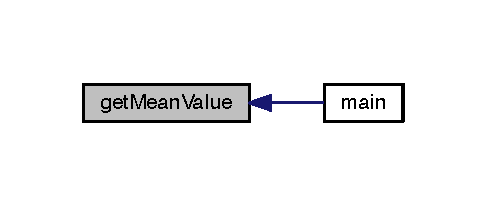
\includegraphics[width=233pt]{d5/d78/_circular_mean_8c_a521968471dd1466d7efc8deb9fb14118_icgraph}
\end{center}
\end{figure}


\index{Circular\+Mean.\+c@{Circular\+Mean.\+c}!init\+Circular\+Mean@{init\+Circular\+Mean}}
\index{init\+Circular\+Mean@{init\+Circular\+Mean}!Circular\+Mean.\+c@{Circular\+Mean.\+c}}
\paragraph[{\texorpdfstring{init\+Circular\+Mean(struct Circular\+Mean $\ast$buf)}{initCircularMean(struct CircularMean *buf)}}]{\setlength{\rightskip}{0pt plus 5cm}void init\+Circular\+Mean (
\begin{DoxyParamCaption}
\item[{struct {\bf Circular\+Mean} $\ast$}]{buf}
\end{DoxyParamCaption}
)}\hypertarget{_circular_mean_8c_a5118b6b2a8751d4400b4ea2a0a15329a}{}\label{_circular_mean_8c_a5118b6b2a8751d4400b4ea2a0a15329a}


Initialize a \hyperlink{_circular_mean_8h_d2/ddd/struct_circular_mean}{Circular\+Mean} struct. 


\begin{DoxyParams}[1]{Parametre}
\mbox{\tt in}  & {\em buf} & Pointer to the \hyperlink{_circular_mean_8h_d2/ddd/struct_circular_mean}{Circular\+Mean} to initialize\\
\hline
\end{DoxyParams}
\begin{DoxyAuthor}{Forfatter}
Simon Nejmann (\href{mailto:19981127@uni.au.dk}{\tt 19981127@uni.\+au.\+dk}) 
\end{DoxyAuthor}


Defineret på linje 19 i filen Circular\+Mean.\+c.



Indeholder referencer til B\+U\+F\+\_\+\+S\+I\+ZE, Circular\+Mean\+::num, Circular\+Mean\+::queue og Circular\+Mean\+::start.



Refereret til af Sensor\+Data\+::init\+Sensor\+Data().


\begin{DoxyCode}
20 \{
21     \textcolor{keywordtype}{int} i;
22     \textcolor{keywordflow}{for} (i = 0; i < \hyperlink{_circular_mean_8h_a6821bafc3c88dfb2e433a095df9940c6}{BUF\_SIZE}; ++i) \{
23         buf->\hyperlink{_circular_mean_8h_aa72bd937f7340af96c3b815933c02734}{queue}[i] = -1;
24     \}
25     buf->\hyperlink{_circular_mean_8h_a0558edb7889eddddb3a01e3956de01c4}{start} = 0;
26     buf->\hyperlink{_circular_mean_8h_a724393befd13aa885c528e4d1a40d8e7}{num} = 0;
27 \}
\end{DoxyCode}


Her er kalder-\/grafen for denne funktion\+:
\nopagebreak
\begin{figure}[H]
\begin{center}
\leavevmode
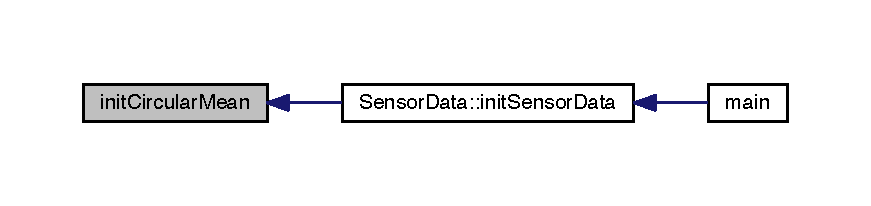
\includegraphics[width=350pt]{d5/d78/_circular_mean_8c_a5118b6b2a8751d4400b4ea2a0a15329a_icgraph}
\end{center}
\end{figure}


\index{Circular\+Mean.\+c@{Circular\+Mean.\+c}!insert\+Value@{insert\+Value}}
\index{insert\+Value@{insert\+Value}!Circular\+Mean.\+c@{Circular\+Mean.\+c}}
\paragraph[{\texorpdfstring{insert\+Value(struct Circular\+Mean $\ast$buf, int val)}{insertValue(struct CircularMean *buf, int val)}}]{\setlength{\rightskip}{0pt plus 5cm}void insert\+Value (
\begin{DoxyParamCaption}
\item[{struct {\bf Circular\+Mean} $\ast$}]{buf, }
\item[{int}]{val}
\end{DoxyParamCaption}
)}\hypertarget{_circular_mean_8c_a6dfc9bb6b16de641325dc73e7f31f7fc}{}\label{_circular_mean_8c_a6dfc9bb6b16de641325dc73e7f31f7fc}


Insert value, possibly overwriting oldest entry. 


\begin{DoxyParams}[1]{Parametre}
\mbox{\tt in}  & {\em buf} & Pointer to the \hyperlink{_circular_mean_8h_d2/ddd/struct_circular_mean}{Circular\+Mean} to insert into \\
\hline
\mbox{\tt in}  & {\em val} & Value to insert\\
\hline
\end{DoxyParams}
\begin{DoxyAuthor}{Forfatter}
Simon Nejmann (\href{mailto:19981127@uni.au.dk}{\tt 19981127@uni.\+au.\+dk}) 
\end{DoxyAuthor}


Defineret på linje 36 i filen Circular\+Mean.\+c.



Indeholder referencer til B\+U\+F\+\_\+\+S\+I\+ZE, Circular\+Mean\+::num, Circular\+Mean\+::queue og Circular\+Mean\+::start.



Refereret til af main().


\begin{DoxyCode}
37 \{
38     buf->\hyperlink{_circular_mean_8h_aa72bd937f7340af96c3b815933c02734}{queue}[buf->\hyperlink{_circular_mean_8h_a0558edb7889eddddb3a01e3956de01c4}{start}] = val;
39     buf->\hyperlink{_circular_mean_8h_a0558edb7889eddddb3a01e3956de01c4}{start} = (buf->\hyperlink{_circular_mean_8h_a0558edb7889eddddb3a01e3956de01c4}{start} +1) % \hyperlink{_circular_mean_8h_a6821bafc3c88dfb2e433a095df9940c6}{BUF\_SIZE};
40     ++(buf->\hyperlink{_circular_mean_8h_a724393befd13aa885c528e4d1a40d8e7}{num});
41     \textcolor{keywordflow}{if} (buf->\hyperlink{_circular_mean_8h_a724393befd13aa885c528e4d1a40d8e7}{num} > \hyperlink{_circular_mean_8h_a6821bafc3c88dfb2e433a095df9940c6}{BUF\_SIZE}) \{
42         buf->\hyperlink{_circular_mean_8h_a724393befd13aa885c528e4d1a40d8e7}{num} = \hyperlink{_circular_mean_8h_a6821bafc3c88dfb2e433a095df9940c6}{BUF\_SIZE};
43     \}
44 \}
\end{DoxyCode}


Her er kalder-\/grafen for denne funktion\+:
\nopagebreak
\begin{figure}[H]
\begin{center}
\leavevmode
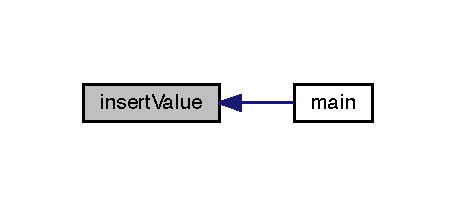
\includegraphics[width=219pt]{d5/d78/_circular_mean_8c_a6dfc9bb6b16de641325dc73e7f31f7fc_icgraph}
\end{center}
\end{figure}



\hypertarget{_circular_mean_8h}{}\subsection{Circular\+Mean.\+h filreference}
\label{_circular_mean_8h}\index{Circular\+Mean.\+h@{Circular\+Mean.\+h}}


Circular buffer used for calculating the average of a series of values. \hyperlink{class_queue}{Queue} is circular and can contain B\+U\+F\+\_\+\+S\+I\+ZE elements. start points to the next element to overwrite. num is the number of items inserted -\/ it grows to B\+U\+F\+\_\+\+S\+I\+ZE and then stays there.  


Denne graf viser, hvilke filer der direkte eller indirekte inkluderer denne fil\+:\nopagebreak
\begin{figure}[H]
\begin{center}
\leavevmode
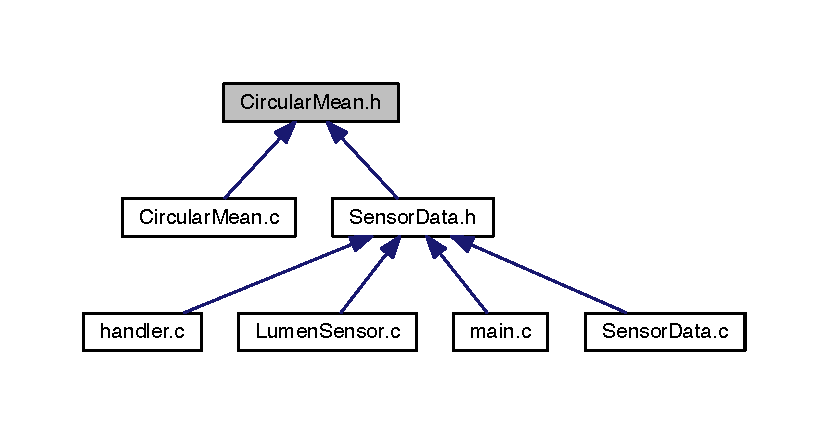
\includegraphics[width=350pt]{_circular_mean_8h__dep__incl}
\end{center}
\end{figure}
\subsubsection*{Datastrukturer}
\begin{DoxyCompactItemize}
\item 
class \hyperlink{_circular_mean_8h_struct_circular_mean}{Circular\+Mean}
\begin{DoxyCompactList}\small\item\em Struct for the buffer.  \hyperlink{_circular_mean_8h_struct_circular_mean}{Mere...}\end{DoxyCompactList}\end{DoxyCompactItemize}
\subsubsection*{\#Defines}
\begin{DoxyCompactItemize}
\item 
\#define \hyperlink{_circular_mean_8h_a6821bafc3c88dfb2e433a095df9940c6}{B\+U\+F\+\_\+\+S\+I\+ZE}~30
\end{DoxyCompactItemize}
\subsubsection*{Funktioner}
\begin{DoxyCompactItemize}
\item 
void \hyperlink{_circular_mean_8h_a5118b6b2a8751d4400b4ea2a0a15329a}{init\+Circular\+Mean} (struct \hyperlink{_circular_mean_8h_struct_circular_mean}{Circular\+Mean} $\ast$buf)
\begin{DoxyCompactList}\small\item\em Initialize a \hyperlink{_circular_mean_8h_struct_circular_mean}{Circular\+Mean} struct. \end{DoxyCompactList}\item 
void \hyperlink{_circular_mean_8h_a6dfc9bb6b16de641325dc73e7f31f7fc}{insert\+Value} (struct \hyperlink{_circular_mean_8h_struct_circular_mean}{Circular\+Mean} $\ast$buf, int val)
\begin{DoxyCompactList}\small\item\em Insert value, possibly overwriting oldest entry. \end{DoxyCompactList}\item 
int \hyperlink{_circular_mean_8h_a521968471dd1466d7efc8deb9fb14118}{get\+Mean\+Value} (struct \hyperlink{_circular_mean_8h_struct_circular_mean}{Circular\+Mean} $\ast$buf)
\begin{DoxyCompactList}\small\item\em Get the average value of all the ints in the buffer. \end{DoxyCompactList}\end{DoxyCompactItemize}


\subsubsection{Detaljeret beskrivelse}
Circular buffer used for calculating the average of a series of values. \hyperlink{class_queue}{Queue} is circular and can contain B\+U\+F\+\_\+\+S\+I\+ZE elements. start points to the next element to overwrite. num is the number of items inserted -\/ it grows to B\+U\+F\+\_\+\+S\+I\+ZE and then stays there. 

\begin{DoxyAuthor}{Forfatter}
Simon Nejmann (\href{mailto:19981127@uni.au.dk}{\tt 19981127@uni.\+au.\+dk})
\end{DoxyAuthor}


\subsubsection{Datastruktur-\/documentation}
\index{Circular\+Mean@{Circular\+Mean}}\label{struct_circular_mean}
\hypertarget{_circular_mean_8h_struct_circular_mean}{}
\paragraph{class Circular\+Mean}
Struct for the buffer. 

Circular buffer used for calculating the average of a series of values.

\begin{DoxyAuthor}{Forfatter}
Simon Nejmann (\href{mailto:19981127@uni.au.dk}{\tt 19981127@uni.\+au.\+dk}) 
\end{DoxyAuthor}


Defineret på linje 17 i filen Circular\+Mean.\+h.



Samarbejdsdiagram for Circular\+Mean\+:\nopagebreak
\begin{figure}[H]
\begin{center}
\leavevmode
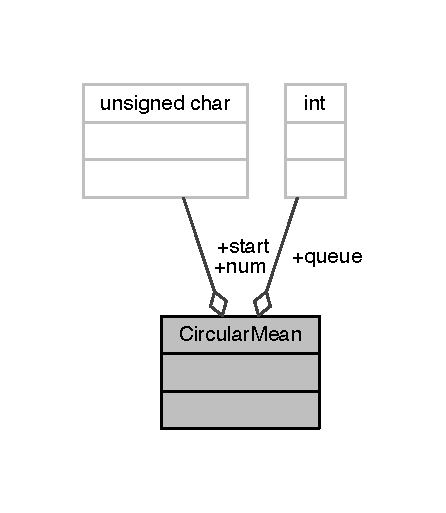
\includegraphics[width=214pt]{struct_circular_mean__coll__graph}
\end{center}
\end{figure}
\begin{DoxyFields}{Data-\/felter}
unsigned char\hypertarget{_circular_mean_8h_a724393befd13aa885c528e4d1a40d8e7}{}\label{_circular_mean_8h_a724393befd13aa885c528e4d1a40d8e7}
&
num&
Number of values current in the array \\
\hline

int\hypertarget{_circular_mean_8h_aa72bd937f7340af96c3b815933c02734}{}\label{_circular_mean_8h_aa72bd937f7340af96c3b815933c02734}
&
queue\mbox{[}\hyperlink{_circular_mean_8h_a6821bafc3c88dfb2e433a095df9940c6}{B\+U\+F\+\_\+\+S\+I\+ZE}\mbox{]}&
Array holding the inserted values \\
\hline

unsigned char\hypertarget{_circular_mean_8h_a0558edb7889eddddb3a01e3956de01c4}{}\label{_circular_mean_8h_a0558edb7889eddddb3a01e3956de01c4}
&
start&
Points to the next array-\/cell to write in \\
\hline

\end{DoxyFields}


\subsubsection{\#Define-\/dokumentation}
\index{Circular\+Mean.\+h@{Circular\+Mean.\+h}!B\+U\+F\+\_\+\+S\+I\+ZE@{B\+U\+F\+\_\+\+S\+I\+ZE}}
\index{B\+U\+F\+\_\+\+S\+I\+ZE@{B\+U\+F\+\_\+\+S\+I\+ZE}!Circular\+Mean.\+h@{Circular\+Mean.\+h}}
\paragraph[{\texorpdfstring{B\+U\+F\+\_\+\+S\+I\+ZE}{BUF_SIZE}}]{\setlength{\rightskip}{0pt plus 5cm}\#define B\+U\+F\+\_\+\+S\+I\+ZE~30}\hypertarget{_circular_mean_8h_a6821bafc3c88dfb2e433a095df9940c6}{}\label{_circular_mean_8h_a6821bafc3c88dfb2e433a095df9940c6}
The size of the buffer. Max 255 

Defineret på linje 12 i filen Circular\+Mean.\+h.



Refereret til af init\+Circular\+Mean() og insert\+Value().



\subsubsection{Funktions-\/dokumentation}
\index{Circular\+Mean.\+h@{Circular\+Mean.\+h}!get\+Mean\+Value@{get\+Mean\+Value}}
\index{get\+Mean\+Value@{get\+Mean\+Value}!Circular\+Mean.\+h@{Circular\+Mean.\+h}}
\paragraph[{\texorpdfstring{get\+Mean\+Value(struct Circular\+Mean $\ast$buf)}{getMeanValue(struct CircularMean *buf)}}]{\setlength{\rightskip}{0pt plus 5cm}int get\+Mean\+Value (
\begin{DoxyParamCaption}
\item[{struct {\bf Circular\+Mean} $\ast$}]{buf}
\end{DoxyParamCaption}
)}\hypertarget{_circular_mean_8h_a521968471dd1466d7efc8deb9fb14118}{}\label{_circular_mean_8h_a521968471dd1466d7efc8deb9fb14118}


Get the average value of all the ints in the buffer. 


\begin{DoxyParams}[1]{Parametre}
\mbox{\tt in}  & {\em buf} & Pointer to the \hyperlink{_circular_mean_8h_struct_circular_mean}{Circular\+Mean} \\
\hline
\end{DoxyParams}
\begin{DoxyReturn}{Returnerer}
The average value calculated
\end{DoxyReturn}
\begin{DoxyAuthor}{Forfatter}
Simon Nejmann (\href{mailto:19981127@uni.au.dk}{\tt 19981127@uni.\+au.\+dk}) 
\end{DoxyAuthor}


Defineret på linje 53 i filen Circular\+Mean.\+c.



Indeholder referencer til Circular\+Mean\+::num og Circular\+Mean\+::queue.



Refereret til af main().


\begin{DoxyCode}
54 \{
55     \textcolor{keywordflow}{if} (buf->\hyperlink{_circular_mean_8h_a724393befd13aa885c528e4d1a40d8e7}{num} == 0)
56         \textcolor{keywordflow}{return} 0;
57 
58     \textcolor{keywordtype}{int} i, temp = 0;
59     \textcolor{keywordflow}{for} (i = 0; i < buf->\hyperlink{_circular_mean_8h_a724393befd13aa885c528e4d1a40d8e7}{num}; ++i) \{
60         temp += buf->\hyperlink{_circular_mean_8h_aa72bd937f7340af96c3b815933c02734}{queue}[i];
61     \}
62 
63     \textcolor{keywordflow}{return} temp / buf->\hyperlink{_circular_mean_8h_a724393befd13aa885c528e4d1a40d8e7}{num};
64 \}
\end{DoxyCode}


Her er kalder-\/grafen for denne funktion\+:\nopagebreak
\begin{figure}[H]
\begin{center}
\leavevmode
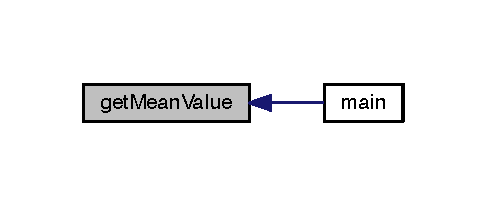
\includegraphics[width=233pt]{_circular_mean_8h_a521968471dd1466d7efc8deb9fb14118_icgraph}
\end{center}
\end{figure}


\index{Circular\+Mean.\+h@{Circular\+Mean.\+h}!init\+Circular\+Mean@{init\+Circular\+Mean}}
\index{init\+Circular\+Mean@{init\+Circular\+Mean}!Circular\+Mean.\+h@{Circular\+Mean.\+h}}
\paragraph[{\texorpdfstring{init\+Circular\+Mean(struct Circular\+Mean $\ast$buf)}{initCircularMean(struct CircularMean *buf)}}]{\setlength{\rightskip}{0pt plus 5cm}void init\+Circular\+Mean (
\begin{DoxyParamCaption}
\item[{struct {\bf Circular\+Mean} $\ast$}]{buf}
\end{DoxyParamCaption}
)}\hypertarget{_circular_mean_8h_a5118b6b2a8751d4400b4ea2a0a15329a}{}\label{_circular_mean_8h_a5118b6b2a8751d4400b4ea2a0a15329a}


Initialize a \hyperlink{_circular_mean_8h_struct_circular_mean}{Circular\+Mean} struct. 


\begin{DoxyParams}[1]{Parametre}
\mbox{\tt in}  & {\em buf} & Pointer to the \hyperlink{_circular_mean_8h_struct_circular_mean}{Circular\+Mean} to initialize\\
\hline
\end{DoxyParams}
\begin{DoxyAuthor}{Forfatter}
Simon Nejmann (\href{mailto:19981127@uni.au.dk}{\tt 19981127@uni.\+au.\+dk}) 
\end{DoxyAuthor}


Defineret på linje 19 i filen Circular\+Mean.\+c.



Indeholder referencer til B\+U\+F\+\_\+\+S\+I\+ZE, Circular\+Mean\+::num, Circular\+Mean\+::queue og Circular\+Mean\+::start.



Refereret til af Sensor\+Data\+::init\+Sensor\+Data().


\begin{DoxyCode}
20 \{
21     \textcolor{keywordtype}{int} i;
22     \textcolor{keywordflow}{for} (i = 0; i < \hyperlink{_circular_mean_8h_a6821bafc3c88dfb2e433a095df9940c6}{BUF\_SIZE}; ++i) \{
23         buf->\hyperlink{_circular_mean_8h_aa72bd937f7340af96c3b815933c02734}{queue}[i] = -1;
24     \}
25     buf->\hyperlink{_circular_mean_8h_a0558edb7889eddddb3a01e3956de01c4}{start} = 0;
26     buf->\hyperlink{_circular_mean_8h_a724393befd13aa885c528e4d1a40d8e7}{num} = 0;
27 \}
\end{DoxyCode}


Her er kalder-\/grafen for denne funktion\+:\nopagebreak
\begin{figure}[H]
\begin{center}
\leavevmode
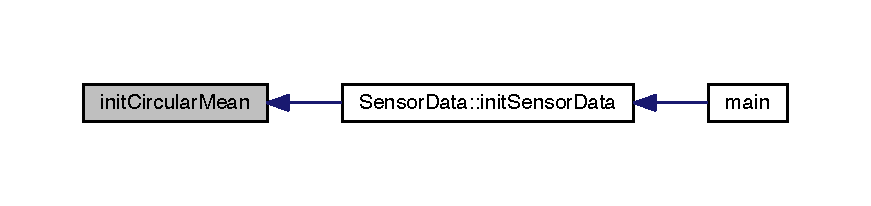
\includegraphics[width=350pt]{_circular_mean_8h_a5118b6b2a8751d4400b4ea2a0a15329a_icgraph}
\end{center}
\end{figure}


\index{Circular\+Mean.\+h@{Circular\+Mean.\+h}!insert\+Value@{insert\+Value}}
\index{insert\+Value@{insert\+Value}!Circular\+Mean.\+h@{Circular\+Mean.\+h}}
\paragraph[{\texorpdfstring{insert\+Value(struct Circular\+Mean $\ast$buf, int val)}{insertValue(struct CircularMean *buf, int val)}}]{\setlength{\rightskip}{0pt plus 5cm}void insert\+Value (
\begin{DoxyParamCaption}
\item[{struct {\bf Circular\+Mean} $\ast$}]{buf, }
\item[{int}]{val}
\end{DoxyParamCaption}
)}\hypertarget{_circular_mean_8h_a6dfc9bb6b16de641325dc73e7f31f7fc}{}\label{_circular_mean_8h_a6dfc9bb6b16de641325dc73e7f31f7fc}


Insert value, possibly overwriting oldest entry. 


\begin{DoxyParams}[1]{Parametre}
\mbox{\tt in}  & {\em buf} & Pointer to the \hyperlink{_circular_mean_8h_struct_circular_mean}{Circular\+Mean} to insert into \\
\hline
\mbox{\tt in}  & {\em val} & Value to insert\\
\hline
\end{DoxyParams}
\begin{DoxyAuthor}{Forfatter}
Simon Nejmann (\href{mailto:19981127@uni.au.dk}{\tt 19981127@uni.\+au.\+dk}) 
\end{DoxyAuthor}


Defineret på linje 36 i filen Circular\+Mean.\+c.



Indeholder referencer til B\+U\+F\+\_\+\+S\+I\+ZE, Circular\+Mean\+::num, Circular\+Mean\+::queue og Circular\+Mean\+::start.



Refereret til af main().


\begin{DoxyCode}
37 \{
38     buf->\hyperlink{_circular_mean_8h_aa72bd937f7340af96c3b815933c02734}{queue}[buf->\hyperlink{_circular_mean_8h_a0558edb7889eddddb3a01e3956de01c4}{start}] = val;
39     buf->\hyperlink{_circular_mean_8h_a0558edb7889eddddb3a01e3956de01c4}{start} = (buf->\hyperlink{_circular_mean_8h_a0558edb7889eddddb3a01e3956de01c4}{start} +1) % \hyperlink{_circular_mean_8h_a6821bafc3c88dfb2e433a095df9940c6}{BUF\_SIZE};
40     ++(buf->\hyperlink{_circular_mean_8h_a724393befd13aa885c528e4d1a40d8e7}{num});
41     \textcolor{keywordflow}{if} (buf->\hyperlink{_circular_mean_8h_a724393befd13aa885c528e4d1a40d8e7}{num} > \hyperlink{_circular_mean_8h_a6821bafc3c88dfb2e433a095df9940c6}{BUF\_SIZE}) \{
42         buf->\hyperlink{_circular_mean_8h_a724393befd13aa885c528e4d1a40d8e7}{num} = \hyperlink{_circular_mean_8h_a6821bafc3c88dfb2e433a095df9940c6}{BUF\_SIZE};
43     \}
44 \}
\end{DoxyCode}


Her er kalder-\/grafen for denne funktion\+:\nopagebreak
\begin{figure}[H]
\begin{center}
\leavevmode
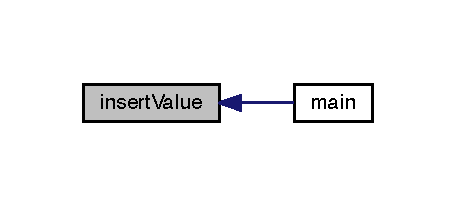
\includegraphics[width=219pt]{_circular_mean_8h_a6dfc9bb6b16de641325dc73e7f31f7fc_icgraph}
\end{center}
\end{figure}



\hypertarget{cyapicallbacks_8h}{}\subsection{cyapicallbacks.\+h filreference}
\label{cyapicallbacks_8h}\index{cyapicallbacks.\+h@{cyapicallbacks.\+h}}
Denne graf viser, hvilke filer der direkte eller indirekte inkluderer denne fil\+:
\nopagebreak
\begin{figure}[H]
\begin{center}
\leavevmode
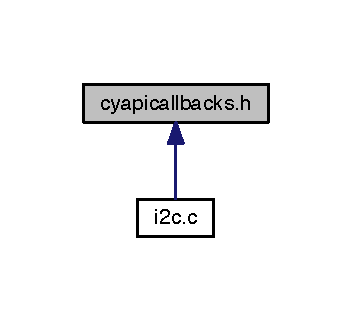
\includegraphics[width=169pt]{d4/d7d/cyapicallbacks_8h__dep__incl}
\end{center}
\end{figure}
\subsubsection*{\#Defines}
\begin{DoxyCompactItemize}
\item 
\#define \hyperlink{cyapicallbacks_8h_a696f67b7d6a9c9a1dac6387ac85b0159}{I2\+C\+S\+\_\+\+I2\+C\+\_\+\+I\+S\+R\+\_\+\+E\+X\+I\+T\+\_\+\+C\+A\+L\+L\+B\+A\+CK}
\end{DoxyCompactItemize}
\subsubsection*{Funktioner}
\begin{DoxyCompactItemize}
\item 
void \hyperlink{cyapicallbacks_8h_ab1cc1a553a438e7390297df1a2181173}{I2\+C\+S\+\_\+\+I2\+C\+\_\+\+I\+S\+R\+\_\+\+Exit\+Callback} (void)
\end{DoxyCompactItemize}


\subsubsection{\#Define-\/dokumentation}
\index{cyapicallbacks.\+h@{cyapicallbacks.\+h}!I2\+C\+S\+\_\+\+I2\+C\+\_\+\+I\+S\+R\+\_\+\+E\+X\+I\+T\+\_\+\+C\+A\+L\+L\+B\+A\+CK@{I2\+C\+S\+\_\+\+I2\+C\+\_\+\+I\+S\+R\+\_\+\+E\+X\+I\+T\+\_\+\+C\+A\+L\+L\+B\+A\+CK}}
\index{I2\+C\+S\+\_\+\+I2\+C\+\_\+\+I\+S\+R\+\_\+\+E\+X\+I\+T\+\_\+\+C\+A\+L\+L\+B\+A\+CK@{I2\+C\+S\+\_\+\+I2\+C\+\_\+\+I\+S\+R\+\_\+\+E\+X\+I\+T\+\_\+\+C\+A\+L\+L\+B\+A\+CK}!cyapicallbacks.\+h@{cyapicallbacks.\+h}}
\paragraph[{\texorpdfstring{I2\+C\+S\+\_\+\+I2\+C\+\_\+\+I\+S\+R\+\_\+\+E\+X\+I\+T\+\_\+\+C\+A\+L\+L\+B\+A\+CK}{I2CS_I2C_ISR_EXIT_CALLBACK}}]{\setlength{\rightskip}{0pt plus 5cm}\#define I2\+C\+S\+\_\+\+I2\+C\+\_\+\+I\+S\+R\+\_\+\+E\+X\+I\+T\+\_\+\+C\+A\+L\+L\+B\+A\+CK}\hypertarget{cyapicallbacks_8h_a696f67b7d6a9c9a1dac6387ac85b0159}{}\label{cyapicallbacks_8h_a696f67b7d6a9c9a1dac6387ac85b0159}


Defineret på linje 15 i filen cyapicallbacks.\+h.



\subsubsection{Funktions-\/dokumentation}
\index{cyapicallbacks.\+h@{cyapicallbacks.\+h}!I2\+C\+S\+\_\+\+I2\+C\+\_\+\+I\+S\+R\+\_\+\+Exit\+Callback@{I2\+C\+S\+\_\+\+I2\+C\+\_\+\+I\+S\+R\+\_\+\+Exit\+Callback}}
\index{I2\+C\+S\+\_\+\+I2\+C\+\_\+\+I\+S\+R\+\_\+\+Exit\+Callback@{I2\+C\+S\+\_\+\+I2\+C\+\_\+\+I\+S\+R\+\_\+\+Exit\+Callback}!cyapicallbacks.\+h@{cyapicallbacks.\+h}}
\paragraph[{\texorpdfstring{I2\+C\+S\+\_\+\+I2\+C\+\_\+\+I\+S\+R\+\_\+\+Exit\+Callback(void)}{I2CS_I2C_ISR_ExitCallback(void)}}]{\setlength{\rightskip}{0pt plus 5cm}void I2\+C\+S\+\_\+\+I2\+C\+\_\+\+I\+S\+R\+\_\+\+Exit\+Callback (
\begin{DoxyParamCaption}
\item[{void}]{}
\end{DoxyParamCaption}
)}\hypertarget{cyapicallbacks_8h_ab1cc1a553a438e7390297df1a2181173}{}\label{cyapicallbacks_8h_ab1cc1a553a438e7390297df1a2181173}

\hypertarget{handler_8c}{}\subsection{handler.\+c filreference}
\label{handler_8c}\index{handler.\+c@{handler.\+c}}


\hyperlink{class_handler}{Handler} modul.  


{\ttfamily \#include \char`\"{}handler.\+h\char`\"{}}\\*
{\ttfamily \#include \char`\"{}data.\+h\char`\"{}}\\*
{\ttfamily \#include \char`\"{}i2c.\+h\char`\"{}}\\*
{\ttfamily \#include \char`\"{}spi.\+h\char`\"{}}\\*
{\ttfamily \#include $<$stdio.\+h$>$}\\*
Inklusions-\/afhængighedsgraf for handler.\+c\+:\nopagebreak
\begin{figure}[H]
\begin{center}
\leavevmode
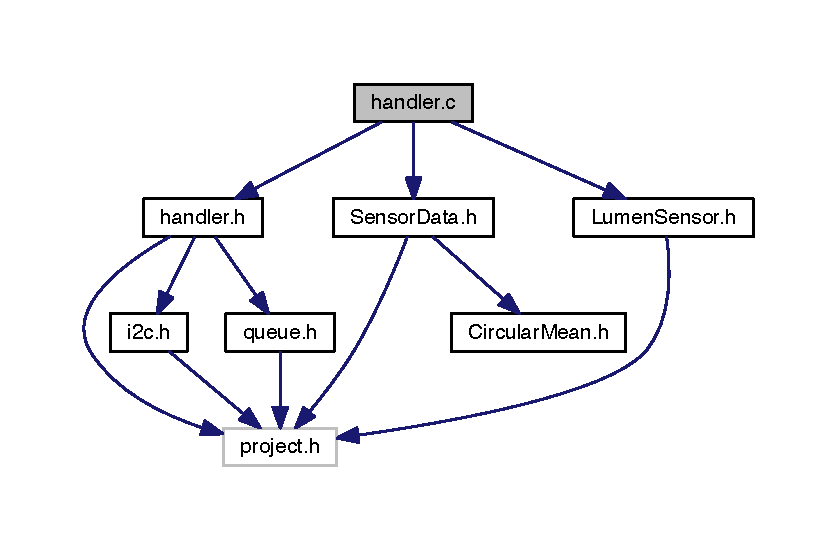
\includegraphics[width=350pt]{d2/d83/handler_8c__incl}
\end{center}
\end{figure}


\subsubsection{Detaljeret beskrivelse}
\hyperlink{class_handler}{Handler} modul. 

Håndtere indkommende kommandoer med tilhørende værdier. \begin{DoxyAuthor}{Forfatter}
Jeppe Stærk Antonsen (\href{mailto:201271201@uni.au.dk}{\tt 201271201@uni.\+au.\+dk}) 
\end{DoxyAuthor}

\hypertarget{handler_8h}{}\subsection{handler.\+h filreference}
\label{handler_8h}\index{handler.\+h@{handler.\+h}}


\hyperlink{class_handler}{Handler} modul.  


{\ttfamily \#include $<$project.\+h$>$}\\*
Inklusions-\/afhængighedsgraf for handler.\+h\+:
\nopagebreak
\begin{figure}[H]
\begin{center}
\leavevmode
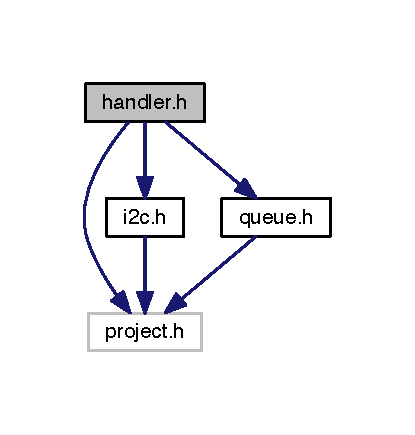
\includegraphics[width=137pt]{db/d41/handler_8h__incl}
\end{center}
\end{figure}
Denne graf viser, hvilke filer der direkte eller indirekte inkluderer denne fil\+:
\nopagebreak
\begin{figure}[H]
\begin{center}
\leavevmode
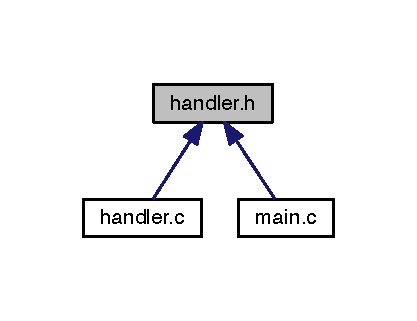
\includegraphics[width=255pt]{d4/d76/handler_8h__dep__incl}
\end{center}
\end{figure}
\subsubsection*{\#Defines}
\begin{DoxyCompactItemize}
\item 
\#define \hyperlink{handler_8h_af70b73890a98cfe329a916df037f46a4}{C\+M\+D\+\_\+\+S\+E\+T\+\_\+\+X\+\_\+\+P\+OS}~(0x10u)
\item 
\#define \hyperlink{handler_8h_a82640a671f668fb40ff4851901d5a151}{C\+M\+D\+\_\+\+S\+E\+T\+\_\+\+Y\+\_\+\+P\+OS}~(0x11u)
\item 
\#define \hyperlink{handler_8h_aa50e083669624eeaef782ebc867008f9}{C\+M\+D\+\_\+\+G\+E\+T\+\_\+\+X\+\_\+\+P\+OS}~(0x12u)
\item 
\#define \hyperlink{handler_8h_a51053e5251048d6ebbf4d2e23de40761}{C\+M\+D\+\_\+\+G\+E\+T\+\_\+\+Y\+\_\+\+P\+OS}~(0x13u)
\item 
\#define \hyperlink{handler_8h_ad9bda4ca0abdec2ab1e6506761623671}{C\+M\+D\+\_\+\+G\+E\+T\+\_\+\+X\+\_\+\+M\+AX}~(0x14u)
\item 
\#define \hyperlink{handler_8h_ab73a35345dedba2dcb9641488e8ddadd}{C\+M\+D\+\_\+\+G\+E\+T\+\_\+\+Y\+\_\+\+M\+AX}~(0x15u)
\item 
\#define \hyperlink{handler_8h_af7c8f19d1c1b9e2240251d42109c5cfd}{C\+M\+D\+\_\+\+X\+\_\+\+S\+TP}~(0x16u)
\item 
\#define \hyperlink{handler_8h_a83ab3037b2c91ea010b2d8c47acd5434}{C\+M\+D\+\_\+\+Y\+\_\+\+S\+TP}~(0x17u)
\item 
\#define \hyperlink{handler_8h_a5edf35288955238e1090f2367f96e828}{C\+M\+D\+\_\+\+X\+\_\+\+C\+AL}~(0x18u)
\item 
\#define \hyperlink{handler_8h_a2b2db51eef91dc2aa5586d0817838ef2}{C\+M\+D\+\_\+\+Y\+\_\+\+C\+AL}~(0x19u)
\item 
\#define \hyperlink{handler_8h_a6e695093ea021ccac7cc5d2d788095c9}{C\+M\+D\+\_\+\+S\+E\+T\+\_\+\+Z\+\_\+\+P\+OS}~(0x20u)
\item 
\#define \hyperlink{handler_8h_a4d76e78d09a00f75609569d9aa92ab98}{C\+M\+D\+\_\+\+G\+E\+T\+\_\+\+Z\+\_\+\+P\+OS}~(0x21u)
\item 
\#define \hyperlink{handler_8h_a188e7cab5d0cf0e363a20c5abcdab482}{C\+M\+D\+\_\+\+G\+E\+T\+\_\+\+Z\+\_\+\+M\+AX}~(0x22u)
\item 
\#define \hyperlink{handler_8h_ad119aef78e8cb8e9aa12f35aeae94a99}{C\+M\+D\+\_\+\+Z\+\_\+\+S\+TP}~(0x23u)
\item 
\#define \hyperlink{handler_8h_ab77bdaae57e9e34f7bfc1d1a31213f94}{C\+M\+D\+\_\+\+Z\+\_\+\+C\+AL}~(0x24u)
\item 
\#define \hyperlink{handler_8h_afc24de4a99d70315d939185a1c3d61f0}{C\+M\+D\+\_\+\+S\+E\+T\+\_\+\+R\+E\+D\+\_\+\+V\+AL}~(0x30u)
\item 
\#define \hyperlink{handler_8h_a24acd29fea2e546409449638b79ac094}{C\+M\+D\+\_\+\+S\+E\+T\+\_\+\+G\+R\+E\+E\+N\+\_\+\+V\+AL}~(0x31u)
\item 
\#define \hyperlink{handler_8h_a4ab3ea64ee56aef3a566698b8959df51}{C\+M\+D\+\_\+\+S\+E\+T\+\_\+\+B\+L\+U\+E\+\_\+\+V\+AL}~(0x32u)
\item 
\#define \hyperlink{handler_8h_a3f217d17f4b67e6b46eb294ab3db2e87}{C\+M\+D\+\_\+\+S\+E\+T\+\_\+\+L\+U\+M\+E\+N\+\_\+\+V\+AL}~(0x33u)
\item 
\#define \hyperlink{handler_8h_a1fe6f15c7c98032dc2bd2a1417977fcf}{C\+M\+D\+\_\+\+S\+E\+T\+\_\+\+P\+O\+W\+E\+R\+\_\+\+S\+TS}~(0x34u)
\item 
\#define \hyperlink{handler_8h_aa2f09e60c4eeae4560da88c6b1b08c60}{C\+M\+D\+\_\+\+G\+E\+T\+\_\+\+R\+E\+D\+\_\+\+V\+AL}~(0x35u)
\item 
\#define \hyperlink{handler_8h_a55d24f50aeb52afddd491d97a66c81ef}{C\+M\+D\+\_\+\+G\+E\+T\+\_\+\+G\+R\+E\+E\+N\+\_\+\+V\+AL}~(0x36u)
\item 
\#define \hyperlink{handler_8h_a81052c67f996705d7eacfcea66bdde08}{C\+M\+D\+\_\+\+G\+E\+T\+\_\+\+B\+L\+U\+E\+\_\+\+V\+AL}~(0x37u)
\item 
\#define \hyperlink{handler_8h_a8ed7ad21a658c878390e9cec4d45aab5}{C\+M\+D\+\_\+\+G\+E\+T\+\_\+\+L\+U\+M\+E\+N\+\_\+\+V\+AL}~(0x38u)
\item 
\#define \hyperlink{handler_8h_ab9e8683e41e93fd467b170c321a1c685}{C\+M\+D\+\_\+\+G\+E\+T\+\_\+\+P\+O\+W\+E\+R\+\_\+\+S\+TS}~(0x39u)
\item 
\#define \hyperlink{handler_8h_a67cc7e7270e79a6e95be2e25cac29feb}{C\+M\+D\+\_\+\+S\+E\+T\+\_\+\+D\+I\+S\+T\+A\+N\+C\+E\+\_\+\+S\+TS}~(0x40u)
\item 
\#define \hyperlink{handler_8h_a84f8a23b131cb2b163e16889afd9ef85}{C\+M\+D\+\_\+\+S\+E\+T\+\_\+\+M\+O\+V\+E\+M\+E\+N\+T\+\_\+\+S\+TS}~(0x41u)
\item 
\#define \hyperlink{handler_8h_a8ea17eed84662f9389bfa1751c03a4b2}{C\+M\+D\+\_\+\+G\+E\+T\+\_\+\+D\+I\+S\+T\+A\+N\+C\+E\+\_\+\+S\+TS}~(0x42u)
\item 
\#define \hyperlink{handler_8h_a4adcfb68de1b319e19342143cb61b550}{C\+M\+D\+\_\+\+G\+E\+T\+\_\+\+M\+O\+V\+E\+M\+E\+N\+T\+\_\+\+S\+TS}~(0x43u)
\item 
\#define \hyperlink{handler_8h_a17dc606d3dbd6f9d4ca831cb02c91af0}{C\+M\+D\+\_\+\+D\+I\+S\+T\+A\+N\+C\+E\+\_\+\+A\+L\+RT}~(0x44u)
\item 
\#define \hyperlink{handler_8h_a7bd43223cfa796f0289d0548e090bbcc}{C\+M\+D\+\_\+\+M\+O\+V\+E\+M\+E\+N\+T\+\_\+\+A\+L\+RT}~(0x45u)
\end{DoxyCompactItemize}
\subsubsection*{Funktioner}
\begin{DoxyCompactItemize}
\item 
void \hyperlink{handler_8h_af5be5b016b862943cd22504490acc8f4}{handler} (uint8 cmd, uint8 val)
\end{DoxyCompactItemize}


\subsubsection{Detaljeret beskrivelse}
\hyperlink{class_handler}{Handler} modul. 

Håndtere indkommende kommandoer med tilhørende værdier. \begin{DoxyAuthor}{Forfatter}
Jeppe Stærk Antonsen (\href{mailto:201271201@uni.au.dk}{\tt 201271201@uni.\+au.\+dk}) 
\end{DoxyAuthor}


\subsubsection{\#Define-\/dokumentation}
\index{handler.\+h@{handler.\+h}!C\+M\+D\+\_\+\+D\+I\+S\+T\+A\+N\+C\+E\+\_\+\+A\+L\+RT@{C\+M\+D\+\_\+\+D\+I\+S\+T\+A\+N\+C\+E\+\_\+\+A\+L\+RT}}
\index{C\+M\+D\+\_\+\+D\+I\+S\+T\+A\+N\+C\+E\+\_\+\+A\+L\+RT@{C\+M\+D\+\_\+\+D\+I\+S\+T\+A\+N\+C\+E\+\_\+\+A\+L\+RT}!handler.\+h@{handler.\+h}}
\paragraph[{\texorpdfstring{C\+M\+D\+\_\+\+D\+I\+S\+T\+A\+N\+C\+E\+\_\+\+A\+L\+RT}{CMD_DISTANCE_ALRT}}]{\setlength{\rightskip}{0pt plus 5cm}\#define C\+M\+D\+\_\+\+D\+I\+S\+T\+A\+N\+C\+E\+\_\+\+A\+L\+RT~(0x44u)}\hypertarget{handler_8h_a17dc606d3dbd6f9d4ca831cb02c91af0}{}\label{handler_8h_a17dc606d3dbd6f9d4ca831cb02c91af0}


Defineret på linje 65 i filen handler.\+h.



Refereret til af Handler\+::handler().

\index{handler.\+h@{handler.\+h}!C\+M\+D\+\_\+\+G\+E\+T\+\_\+\+B\+L\+U\+E\+\_\+\+V\+AL@{C\+M\+D\+\_\+\+G\+E\+T\+\_\+\+B\+L\+U\+E\+\_\+\+V\+AL}}
\index{C\+M\+D\+\_\+\+G\+E\+T\+\_\+\+B\+L\+U\+E\+\_\+\+V\+AL@{C\+M\+D\+\_\+\+G\+E\+T\+\_\+\+B\+L\+U\+E\+\_\+\+V\+AL}!handler.\+h@{handler.\+h}}
\paragraph[{\texorpdfstring{C\+M\+D\+\_\+\+G\+E\+T\+\_\+\+B\+L\+U\+E\+\_\+\+V\+AL}{CMD_GET_BLUE_VAL}}]{\setlength{\rightskip}{0pt plus 5cm}\#define C\+M\+D\+\_\+\+G\+E\+T\+\_\+\+B\+L\+U\+E\+\_\+\+V\+AL~(0x37u)}\hypertarget{handler_8h_a81052c67f996705d7eacfcea66bdde08}{}\label{handler_8h_a81052c67f996705d7eacfcea66bdde08}


Defineret på linje 58 i filen handler.\+h.



Refereret til af S\+P\+I\+::\+C\+Y\+\_\+\+I\+S\+R() og Handler\+::handler().

\index{handler.\+h@{handler.\+h}!C\+M\+D\+\_\+\+G\+E\+T\+\_\+\+D\+I\+S\+T\+A\+N\+C\+E\+\_\+\+S\+TS@{C\+M\+D\+\_\+\+G\+E\+T\+\_\+\+D\+I\+S\+T\+A\+N\+C\+E\+\_\+\+S\+TS}}
\index{C\+M\+D\+\_\+\+G\+E\+T\+\_\+\+D\+I\+S\+T\+A\+N\+C\+E\+\_\+\+S\+TS@{C\+M\+D\+\_\+\+G\+E\+T\+\_\+\+D\+I\+S\+T\+A\+N\+C\+E\+\_\+\+S\+TS}!handler.\+h@{handler.\+h}}
\paragraph[{\texorpdfstring{C\+M\+D\+\_\+\+G\+E\+T\+\_\+\+D\+I\+S\+T\+A\+N\+C\+E\+\_\+\+S\+TS}{CMD_GET_DISTANCE_STS}}]{\setlength{\rightskip}{0pt plus 5cm}\#define C\+M\+D\+\_\+\+G\+E\+T\+\_\+\+D\+I\+S\+T\+A\+N\+C\+E\+\_\+\+S\+TS~(0x42u)}\hypertarget{handler_8h_a8ea17eed84662f9389bfa1751c03a4b2}{}\label{handler_8h_a8ea17eed84662f9389bfa1751c03a4b2}


Defineret på linje 63 i filen handler.\+h.



Refereret til af Handler\+::handler().

\index{handler.\+h@{handler.\+h}!C\+M\+D\+\_\+\+G\+E\+T\+\_\+\+G\+R\+E\+E\+N\+\_\+\+V\+AL@{C\+M\+D\+\_\+\+G\+E\+T\+\_\+\+G\+R\+E\+E\+N\+\_\+\+V\+AL}}
\index{C\+M\+D\+\_\+\+G\+E\+T\+\_\+\+G\+R\+E\+E\+N\+\_\+\+V\+AL@{C\+M\+D\+\_\+\+G\+E\+T\+\_\+\+G\+R\+E\+E\+N\+\_\+\+V\+AL}!handler.\+h@{handler.\+h}}
\paragraph[{\texorpdfstring{C\+M\+D\+\_\+\+G\+E\+T\+\_\+\+G\+R\+E\+E\+N\+\_\+\+V\+AL}{CMD_GET_GREEN_VAL}}]{\setlength{\rightskip}{0pt plus 5cm}\#define C\+M\+D\+\_\+\+G\+E\+T\+\_\+\+G\+R\+E\+E\+N\+\_\+\+V\+AL~(0x36u)}\hypertarget{handler_8h_a55d24f50aeb52afddd491d97a66c81ef}{}\label{handler_8h_a55d24f50aeb52afddd491d97a66c81ef}


Defineret på linje 57 i filen handler.\+h.



Refereret til af S\+P\+I\+::\+C\+Y\+\_\+\+I\+S\+R() og Handler\+::handler().

\index{handler.\+h@{handler.\+h}!C\+M\+D\+\_\+\+G\+E\+T\+\_\+\+L\+U\+M\+E\+N\+\_\+\+V\+AL@{C\+M\+D\+\_\+\+G\+E\+T\+\_\+\+L\+U\+M\+E\+N\+\_\+\+V\+AL}}
\index{C\+M\+D\+\_\+\+G\+E\+T\+\_\+\+L\+U\+M\+E\+N\+\_\+\+V\+AL@{C\+M\+D\+\_\+\+G\+E\+T\+\_\+\+L\+U\+M\+E\+N\+\_\+\+V\+AL}!handler.\+h@{handler.\+h}}
\paragraph[{\texorpdfstring{C\+M\+D\+\_\+\+G\+E\+T\+\_\+\+L\+U\+M\+E\+N\+\_\+\+V\+AL}{CMD_GET_LUMEN_VAL}}]{\setlength{\rightskip}{0pt plus 5cm}\#define C\+M\+D\+\_\+\+G\+E\+T\+\_\+\+L\+U\+M\+E\+N\+\_\+\+V\+AL~(0x38u)}\hypertarget{handler_8h_a8ed7ad21a658c878390e9cec4d45aab5}{}\label{handler_8h_a8ed7ad21a658c878390e9cec4d45aab5}


Defineret på linje 59 i filen handler.\+h.



Refereret til af Handler\+::handler().

\index{handler.\+h@{handler.\+h}!C\+M\+D\+\_\+\+G\+E\+T\+\_\+\+M\+O\+V\+E\+M\+E\+N\+T\+\_\+\+S\+TS@{C\+M\+D\+\_\+\+G\+E\+T\+\_\+\+M\+O\+V\+E\+M\+E\+N\+T\+\_\+\+S\+TS}}
\index{C\+M\+D\+\_\+\+G\+E\+T\+\_\+\+M\+O\+V\+E\+M\+E\+N\+T\+\_\+\+S\+TS@{C\+M\+D\+\_\+\+G\+E\+T\+\_\+\+M\+O\+V\+E\+M\+E\+N\+T\+\_\+\+S\+TS}!handler.\+h@{handler.\+h}}
\paragraph[{\texorpdfstring{C\+M\+D\+\_\+\+G\+E\+T\+\_\+\+M\+O\+V\+E\+M\+E\+N\+T\+\_\+\+S\+TS}{CMD_GET_MOVEMENT_STS}}]{\setlength{\rightskip}{0pt plus 5cm}\#define C\+M\+D\+\_\+\+G\+E\+T\+\_\+\+M\+O\+V\+E\+M\+E\+N\+T\+\_\+\+S\+TS~(0x43u)}\hypertarget{handler_8h_a4adcfb68de1b319e19342143cb61b550}{}\label{handler_8h_a4adcfb68de1b319e19342143cb61b550}


Defineret på linje 64 i filen handler.\+h.



Refereret til af Handler\+::handler().

\index{handler.\+h@{handler.\+h}!C\+M\+D\+\_\+\+G\+E\+T\+\_\+\+P\+O\+W\+E\+R\+\_\+\+S\+TS@{C\+M\+D\+\_\+\+G\+E\+T\+\_\+\+P\+O\+W\+E\+R\+\_\+\+S\+TS}}
\index{C\+M\+D\+\_\+\+G\+E\+T\+\_\+\+P\+O\+W\+E\+R\+\_\+\+S\+TS@{C\+M\+D\+\_\+\+G\+E\+T\+\_\+\+P\+O\+W\+E\+R\+\_\+\+S\+TS}!handler.\+h@{handler.\+h}}
\paragraph[{\texorpdfstring{C\+M\+D\+\_\+\+G\+E\+T\+\_\+\+P\+O\+W\+E\+R\+\_\+\+S\+TS}{CMD_GET_POWER_STS}}]{\setlength{\rightskip}{0pt plus 5cm}\#define C\+M\+D\+\_\+\+G\+E\+T\+\_\+\+P\+O\+W\+E\+R\+\_\+\+S\+TS~(0x39u)}\hypertarget{handler_8h_ab9e8683e41e93fd467b170c321a1c685}{}\label{handler_8h_ab9e8683e41e93fd467b170c321a1c685}


Defineret på linje 60 i filen handler.\+h.



Refereret til af Handler\+::handler().

\index{handler.\+h@{handler.\+h}!C\+M\+D\+\_\+\+G\+E\+T\+\_\+\+R\+E\+D\+\_\+\+V\+AL@{C\+M\+D\+\_\+\+G\+E\+T\+\_\+\+R\+E\+D\+\_\+\+V\+AL}}
\index{C\+M\+D\+\_\+\+G\+E\+T\+\_\+\+R\+E\+D\+\_\+\+V\+AL@{C\+M\+D\+\_\+\+G\+E\+T\+\_\+\+R\+E\+D\+\_\+\+V\+AL}!handler.\+h@{handler.\+h}}
\paragraph[{\texorpdfstring{C\+M\+D\+\_\+\+G\+E\+T\+\_\+\+R\+E\+D\+\_\+\+V\+AL}{CMD_GET_RED_VAL}}]{\setlength{\rightskip}{0pt plus 5cm}\#define C\+M\+D\+\_\+\+G\+E\+T\+\_\+\+R\+E\+D\+\_\+\+V\+AL~(0x35u)}\hypertarget{handler_8h_aa2f09e60c4eeae4560da88c6b1b08c60}{}\label{handler_8h_aa2f09e60c4eeae4560da88c6b1b08c60}


Defineret på linje 56 i filen handler.\+h.



Refereret til af S\+P\+I\+::\+C\+Y\+\_\+\+I\+S\+R() og Handler\+::handler().

\index{handler.\+h@{handler.\+h}!C\+M\+D\+\_\+\+G\+E\+T\+\_\+\+X\+\_\+\+M\+AX@{C\+M\+D\+\_\+\+G\+E\+T\+\_\+\+X\+\_\+\+M\+AX}}
\index{C\+M\+D\+\_\+\+G\+E\+T\+\_\+\+X\+\_\+\+M\+AX@{C\+M\+D\+\_\+\+G\+E\+T\+\_\+\+X\+\_\+\+M\+AX}!handler.\+h@{handler.\+h}}
\paragraph[{\texorpdfstring{C\+M\+D\+\_\+\+G\+E\+T\+\_\+\+X\+\_\+\+M\+AX}{CMD_GET_X_MAX}}]{\setlength{\rightskip}{0pt plus 5cm}\#define C\+M\+D\+\_\+\+G\+E\+T\+\_\+\+X\+\_\+\+M\+AX~(0x14u)}\hypertarget{handler_8h_ad9bda4ca0abdec2ab1e6506761623671}{}\label{handler_8h_ad9bda4ca0abdec2ab1e6506761623671}


Defineret på linje 40 i filen handler.\+h.

\index{handler.\+h@{handler.\+h}!C\+M\+D\+\_\+\+G\+E\+T\+\_\+\+X\+\_\+\+P\+OS@{C\+M\+D\+\_\+\+G\+E\+T\+\_\+\+X\+\_\+\+P\+OS}}
\index{C\+M\+D\+\_\+\+G\+E\+T\+\_\+\+X\+\_\+\+P\+OS@{C\+M\+D\+\_\+\+G\+E\+T\+\_\+\+X\+\_\+\+P\+OS}!handler.\+h@{handler.\+h}}
\paragraph[{\texorpdfstring{C\+M\+D\+\_\+\+G\+E\+T\+\_\+\+X\+\_\+\+P\+OS}{CMD_GET_X_POS}}]{\setlength{\rightskip}{0pt plus 5cm}\#define C\+M\+D\+\_\+\+G\+E\+T\+\_\+\+X\+\_\+\+P\+OS~(0x12u)}\hypertarget{handler_8h_aa50e083669624eeaef782ebc867008f9}{}\label{handler_8h_aa50e083669624eeaef782ebc867008f9}


Defineret på linje 38 i filen handler.\+h.



Refereret til af S\+P\+I\+::\+C\+Y\+\_\+\+I\+S\+R() og Handler\+::handler().

\index{handler.\+h@{handler.\+h}!C\+M\+D\+\_\+\+G\+E\+T\+\_\+\+Y\+\_\+\+M\+AX@{C\+M\+D\+\_\+\+G\+E\+T\+\_\+\+Y\+\_\+\+M\+AX}}
\index{C\+M\+D\+\_\+\+G\+E\+T\+\_\+\+Y\+\_\+\+M\+AX@{C\+M\+D\+\_\+\+G\+E\+T\+\_\+\+Y\+\_\+\+M\+AX}!handler.\+h@{handler.\+h}}
\paragraph[{\texorpdfstring{C\+M\+D\+\_\+\+G\+E\+T\+\_\+\+Y\+\_\+\+M\+AX}{CMD_GET_Y_MAX}}]{\setlength{\rightskip}{0pt plus 5cm}\#define C\+M\+D\+\_\+\+G\+E\+T\+\_\+\+Y\+\_\+\+M\+AX~(0x15u)}\hypertarget{handler_8h_ab73a35345dedba2dcb9641488e8ddadd}{}\label{handler_8h_ab73a35345dedba2dcb9641488e8ddadd}


Defineret på linje 41 i filen handler.\+h.

\index{handler.\+h@{handler.\+h}!C\+M\+D\+\_\+\+G\+E\+T\+\_\+\+Y\+\_\+\+P\+OS@{C\+M\+D\+\_\+\+G\+E\+T\+\_\+\+Y\+\_\+\+P\+OS}}
\index{C\+M\+D\+\_\+\+G\+E\+T\+\_\+\+Y\+\_\+\+P\+OS@{C\+M\+D\+\_\+\+G\+E\+T\+\_\+\+Y\+\_\+\+P\+OS}!handler.\+h@{handler.\+h}}
\paragraph[{\texorpdfstring{C\+M\+D\+\_\+\+G\+E\+T\+\_\+\+Y\+\_\+\+P\+OS}{CMD_GET_Y_POS}}]{\setlength{\rightskip}{0pt plus 5cm}\#define C\+M\+D\+\_\+\+G\+E\+T\+\_\+\+Y\+\_\+\+P\+OS~(0x13u)}\hypertarget{handler_8h_a51053e5251048d6ebbf4d2e23de40761}{}\label{handler_8h_a51053e5251048d6ebbf4d2e23de40761}


Defineret på linje 39 i filen handler.\+h.



Refereret til af S\+P\+I\+::\+C\+Y\+\_\+\+I\+S\+R() og Handler\+::handler().

\index{handler.\+h@{handler.\+h}!C\+M\+D\+\_\+\+G\+E\+T\+\_\+\+Z\+\_\+\+M\+AX@{C\+M\+D\+\_\+\+G\+E\+T\+\_\+\+Z\+\_\+\+M\+AX}}
\index{C\+M\+D\+\_\+\+G\+E\+T\+\_\+\+Z\+\_\+\+M\+AX@{C\+M\+D\+\_\+\+G\+E\+T\+\_\+\+Z\+\_\+\+M\+AX}!handler.\+h@{handler.\+h}}
\paragraph[{\texorpdfstring{C\+M\+D\+\_\+\+G\+E\+T\+\_\+\+Z\+\_\+\+M\+AX}{CMD_GET_Z_MAX}}]{\setlength{\rightskip}{0pt plus 5cm}\#define C\+M\+D\+\_\+\+G\+E\+T\+\_\+\+Z\+\_\+\+M\+AX~(0x22u)}\hypertarget{handler_8h_a188e7cab5d0cf0e363a20c5abcdab482}{}\label{handler_8h_a188e7cab5d0cf0e363a20c5abcdab482}


Defineret på linje 48 i filen handler.\+h.

\index{handler.\+h@{handler.\+h}!C\+M\+D\+\_\+\+G\+E\+T\+\_\+\+Z\+\_\+\+P\+OS@{C\+M\+D\+\_\+\+G\+E\+T\+\_\+\+Z\+\_\+\+P\+OS}}
\index{C\+M\+D\+\_\+\+G\+E\+T\+\_\+\+Z\+\_\+\+P\+OS@{C\+M\+D\+\_\+\+G\+E\+T\+\_\+\+Z\+\_\+\+P\+OS}!handler.\+h@{handler.\+h}}
\paragraph[{\texorpdfstring{C\+M\+D\+\_\+\+G\+E\+T\+\_\+\+Z\+\_\+\+P\+OS}{CMD_GET_Z_POS}}]{\setlength{\rightskip}{0pt plus 5cm}\#define C\+M\+D\+\_\+\+G\+E\+T\+\_\+\+Z\+\_\+\+P\+OS~(0x21u)}\hypertarget{handler_8h_a4d76e78d09a00f75609569d9aa92ab98}{}\label{handler_8h_a4d76e78d09a00f75609569d9aa92ab98}


Defineret på linje 47 i filen handler.\+h.



Refereret til af S\+P\+I\+::\+C\+Y\+\_\+\+I\+S\+R() og Handler\+::handler().

\index{handler.\+h@{handler.\+h}!C\+M\+D\+\_\+\+M\+O\+V\+E\+M\+E\+N\+T\+\_\+\+A\+L\+RT@{C\+M\+D\+\_\+\+M\+O\+V\+E\+M\+E\+N\+T\+\_\+\+A\+L\+RT}}
\index{C\+M\+D\+\_\+\+M\+O\+V\+E\+M\+E\+N\+T\+\_\+\+A\+L\+RT@{C\+M\+D\+\_\+\+M\+O\+V\+E\+M\+E\+N\+T\+\_\+\+A\+L\+RT}!handler.\+h@{handler.\+h}}
\paragraph[{\texorpdfstring{C\+M\+D\+\_\+\+M\+O\+V\+E\+M\+E\+N\+T\+\_\+\+A\+L\+RT}{CMD_MOVEMENT_ALRT}}]{\setlength{\rightskip}{0pt plus 5cm}\#define C\+M\+D\+\_\+\+M\+O\+V\+E\+M\+E\+N\+T\+\_\+\+A\+L\+RT~(0x45u)}\hypertarget{handler_8h_a7bd43223cfa796f0289d0548e090bbcc}{}\label{handler_8h_a7bd43223cfa796f0289d0548e090bbcc}


Defineret på linje 66 i filen handler.\+h.



Refereret til af Handler\+::handler().

\index{handler.\+h@{handler.\+h}!C\+M\+D\+\_\+\+S\+E\+T\+\_\+\+B\+L\+U\+E\+\_\+\+V\+AL@{C\+M\+D\+\_\+\+S\+E\+T\+\_\+\+B\+L\+U\+E\+\_\+\+V\+AL}}
\index{C\+M\+D\+\_\+\+S\+E\+T\+\_\+\+B\+L\+U\+E\+\_\+\+V\+AL@{C\+M\+D\+\_\+\+S\+E\+T\+\_\+\+B\+L\+U\+E\+\_\+\+V\+AL}!handler.\+h@{handler.\+h}}
\paragraph[{\texorpdfstring{C\+M\+D\+\_\+\+S\+E\+T\+\_\+\+B\+L\+U\+E\+\_\+\+V\+AL}{CMD_SET_BLUE_VAL}}]{\setlength{\rightskip}{0pt plus 5cm}\#define C\+M\+D\+\_\+\+S\+E\+T\+\_\+\+B\+L\+U\+E\+\_\+\+V\+AL~(0x32u)}\hypertarget{handler_8h_a4ab3ea64ee56aef3a566698b8959df51}{}\label{handler_8h_a4ab3ea64ee56aef3a566698b8959df51}


Defineret på linje 53 i filen handler.\+h.



Refereret til af Handler\+::handler().

\index{handler.\+h@{handler.\+h}!C\+M\+D\+\_\+\+S\+E\+T\+\_\+\+D\+I\+S\+T\+A\+N\+C\+E\+\_\+\+S\+TS@{C\+M\+D\+\_\+\+S\+E\+T\+\_\+\+D\+I\+S\+T\+A\+N\+C\+E\+\_\+\+S\+TS}}
\index{C\+M\+D\+\_\+\+S\+E\+T\+\_\+\+D\+I\+S\+T\+A\+N\+C\+E\+\_\+\+S\+TS@{C\+M\+D\+\_\+\+S\+E\+T\+\_\+\+D\+I\+S\+T\+A\+N\+C\+E\+\_\+\+S\+TS}!handler.\+h@{handler.\+h}}
\paragraph[{\texorpdfstring{C\+M\+D\+\_\+\+S\+E\+T\+\_\+\+D\+I\+S\+T\+A\+N\+C\+E\+\_\+\+S\+TS}{CMD_SET_DISTANCE_STS}}]{\setlength{\rightskip}{0pt plus 5cm}\#define C\+M\+D\+\_\+\+S\+E\+T\+\_\+\+D\+I\+S\+T\+A\+N\+C\+E\+\_\+\+S\+TS~(0x40u)}\hypertarget{handler_8h_a67cc7e7270e79a6e95be2e25cac29feb}{}\label{handler_8h_a67cc7e7270e79a6e95be2e25cac29feb}


Defineret på linje 61 i filen handler.\+h.



Refereret til af Handler\+::handler().

\index{handler.\+h@{handler.\+h}!C\+M\+D\+\_\+\+S\+E\+T\+\_\+\+G\+R\+E\+E\+N\+\_\+\+V\+AL@{C\+M\+D\+\_\+\+S\+E\+T\+\_\+\+G\+R\+E\+E\+N\+\_\+\+V\+AL}}
\index{C\+M\+D\+\_\+\+S\+E\+T\+\_\+\+G\+R\+E\+E\+N\+\_\+\+V\+AL@{C\+M\+D\+\_\+\+S\+E\+T\+\_\+\+G\+R\+E\+E\+N\+\_\+\+V\+AL}!handler.\+h@{handler.\+h}}
\paragraph[{\texorpdfstring{C\+M\+D\+\_\+\+S\+E\+T\+\_\+\+G\+R\+E\+E\+N\+\_\+\+V\+AL}{CMD_SET_GREEN_VAL}}]{\setlength{\rightskip}{0pt plus 5cm}\#define C\+M\+D\+\_\+\+S\+E\+T\+\_\+\+G\+R\+E\+E\+N\+\_\+\+V\+AL~(0x31u)}\hypertarget{handler_8h_a24acd29fea2e546409449638b79ac094}{}\label{handler_8h_a24acd29fea2e546409449638b79ac094}


Defineret på linje 52 i filen handler.\+h.



Refereret til af Handler\+::handler().

\index{handler.\+h@{handler.\+h}!C\+M\+D\+\_\+\+S\+E\+T\+\_\+\+L\+U\+M\+E\+N\+\_\+\+V\+AL@{C\+M\+D\+\_\+\+S\+E\+T\+\_\+\+L\+U\+M\+E\+N\+\_\+\+V\+AL}}
\index{C\+M\+D\+\_\+\+S\+E\+T\+\_\+\+L\+U\+M\+E\+N\+\_\+\+V\+AL@{C\+M\+D\+\_\+\+S\+E\+T\+\_\+\+L\+U\+M\+E\+N\+\_\+\+V\+AL}!handler.\+h@{handler.\+h}}
\paragraph[{\texorpdfstring{C\+M\+D\+\_\+\+S\+E\+T\+\_\+\+L\+U\+M\+E\+N\+\_\+\+V\+AL}{CMD_SET_LUMEN_VAL}}]{\setlength{\rightskip}{0pt plus 5cm}\#define C\+M\+D\+\_\+\+S\+E\+T\+\_\+\+L\+U\+M\+E\+N\+\_\+\+V\+AL~(0x33u)}\hypertarget{handler_8h_a3f217d17f4b67e6b46eb294ab3db2e87}{}\label{handler_8h_a3f217d17f4b67e6b46eb294ab3db2e87}


Defineret på linje 54 i filen handler.\+h.



Refereret til af Handler\+::handler().

\index{handler.\+h@{handler.\+h}!C\+M\+D\+\_\+\+S\+E\+T\+\_\+\+M\+O\+V\+E\+M\+E\+N\+T\+\_\+\+S\+TS@{C\+M\+D\+\_\+\+S\+E\+T\+\_\+\+M\+O\+V\+E\+M\+E\+N\+T\+\_\+\+S\+TS}}
\index{C\+M\+D\+\_\+\+S\+E\+T\+\_\+\+M\+O\+V\+E\+M\+E\+N\+T\+\_\+\+S\+TS@{C\+M\+D\+\_\+\+S\+E\+T\+\_\+\+M\+O\+V\+E\+M\+E\+N\+T\+\_\+\+S\+TS}!handler.\+h@{handler.\+h}}
\paragraph[{\texorpdfstring{C\+M\+D\+\_\+\+S\+E\+T\+\_\+\+M\+O\+V\+E\+M\+E\+N\+T\+\_\+\+S\+TS}{CMD_SET_MOVEMENT_STS}}]{\setlength{\rightskip}{0pt plus 5cm}\#define C\+M\+D\+\_\+\+S\+E\+T\+\_\+\+M\+O\+V\+E\+M\+E\+N\+T\+\_\+\+S\+TS~(0x41u)}\hypertarget{handler_8h_a84f8a23b131cb2b163e16889afd9ef85}{}\label{handler_8h_a84f8a23b131cb2b163e16889afd9ef85}


Defineret på linje 62 i filen handler.\+h.



Refereret til af Handler\+::handler().

\index{handler.\+h@{handler.\+h}!C\+M\+D\+\_\+\+S\+E\+T\+\_\+\+P\+O\+W\+E\+R\+\_\+\+S\+TS@{C\+M\+D\+\_\+\+S\+E\+T\+\_\+\+P\+O\+W\+E\+R\+\_\+\+S\+TS}}
\index{C\+M\+D\+\_\+\+S\+E\+T\+\_\+\+P\+O\+W\+E\+R\+\_\+\+S\+TS@{C\+M\+D\+\_\+\+S\+E\+T\+\_\+\+P\+O\+W\+E\+R\+\_\+\+S\+TS}!handler.\+h@{handler.\+h}}
\paragraph[{\texorpdfstring{C\+M\+D\+\_\+\+S\+E\+T\+\_\+\+P\+O\+W\+E\+R\+\_\+\+S\+TS}{CMD_SET_POWER_STS}}]{\setlength{\rightskip}{0pt plus 5cm}\#define C\+M\+D\+\_\+\+S\+E\+T\+\_\+\+P\+O\+W\+E\+R\+\_\+\+S\+TS~(0x34u)}\hypertarget{handler_8h_a1fe6f15c7c98032dc2bd2a1417977fcf}{}\label{handler_8h_a1fe6f15c7c98032dc2bd2a1417977fcf}


Defineret på linje 55 i filen handler.\+h.



Refereret til af Handler\+::handler().

\index{handler.\+h@{handler.\+h}!C\+M\+D\+\_\+\+S\+E\+T\+\_\+\+R\+E\+D\+\_\+\+V\+AL@{C\+M\+D\+\_\+\+S\+E\+T\+\_\+\+R\+E\+D\+\_\+\+V\+AL}}
\index{C\+M\+D\+\_\+\+S\+E\+T\+\_\+\+R\+E\+D\+\_\+\+V\+AL@{C\+M\+D\+\_\+\+S\+E\+T\+\_\+\+R\+E\+D\+\_\+\+V\+AL}!handler.\+h@{handler.\+h}}
\paragraph[{\texorpdfstring{C\+M\+D\+\_\+\+S\+E\+T\+\_\+\+R\+E\+D\+\_\+\+V\+AL}{CMD_SET_RED_VAL}}]{\setlength{\rightskip}{0pt plus 5cm}\#define C\+M\+D\+\_\+\+S\+E\+T\+\_\+\+R\+E\+D\+\_\+\+V\+AL~(0x30u)}\hypertarget{handler_8h_afc24de4a99d70315d939185a1c3d61f0}{}\label{handler_8h_afc24de4a99d70315d939185a1c3d61f0}


Defineret på linje 51 i filen handler.\+h.



Refereret til af Handler\+::handler().

\index{handler.\+h@{handler.\+h}!C\+M\+D\+\_\+\+S\+E\+T\+\_\+\+X\+\_\+\+P\+OS@{C\+M\+D\+\_\+\+S\+E\+T\+\_\+\+X\+\_\+\+P\+OS}}
\index{C\+M\+D\+\_\+\+S\+E\+T\+\_\+\+X\+\_\+\+P\+OS@{C\+M\+D\+\_\+\+S\+E\+T\+\_\+\+X\+\_\+\+P\+OS}!handler.\+h@{handler.\+h}}
\paragraph[{\texorpdfstring{C\+M\+D\+\_\+\+S\+E\+T\+\_\+\+X\+\_\+\+P\+OS}{CMD_SET_X_POS}}]{\setlength{\rightskip}{0pt plus 5cm}\#define C\+M\+D\+\_\+\+S\+E\+T\+\_\+\+X\+\_\+\+P\+OS~(0x10u)}\hypertarget{handler_8h_af70b73890a98cfe329a916df037f46a4}{}\label{handler_8h_af70b73890a98cfe329a916df037f46a4}


Defineret på linje 36 i filen handler.\+h.



Refereret til af Handler\+::handler().

\index{handler.\+h@{handler.\+h}!C\+M\+D\+\_\+\+S\+E\+T\+\_\+\+Y\+\_\+\+P\+OS@{C\+M\+D\+\_\+\+S\+E\+T\+\_\+\+Y\+\_\+\+P\+OS}}
\index{C\+M\+D\+\_\+\+S\+E\+T\+\_\+\+Y\+\_\+\+P\+OS@{C\+M\+D\+\_\+\+S\+E\+T\+\_\+\+Y\+\_\+\+P\+OS}!handler.\+h@{handler.\+h}}
\paragraph[{\texorpdfstring{C\+M\+D\+\_\+\+S\+E\+T\+\_\+\+Y\+\_\+\+P\+OS}{CMD_SET_Y_POS}}]{\setlength{\rightskip}{0pt plus 5cm}\#define C\+M\+D\+\_\+\+S\+E\+T\+\_\+\+Y\+\_\+\+P\+OS~(0x11u)}\hypertarget{handler_8h_a82640a671f668fb40ff4851901d5a151}{}\label{handler_8h_a82640a671f668fb40ff4851901d5a151}


Defineret på linje 37 i filen handler.\+h.



Refereret til af Handler\+::handler().

\index{handler.\+h@{handler.\+h}!C\+M\+D\+\_\+\+S\+E\+T\+\_\+\+Z\+\_\+\+P\+OS@{C\+M\+D\+\_\+\+S\+E\+T\+\_\+\+Z\+\_\+\+P\+OS}}
\index{C\+M\+D\+\_\+\+S\+E\+T\+\_\+\+Z\+\_\+\+P\+OS@{C\+M\+D\+\_\+\+S\+E\+T\+\_\+\+Z\+\_\+\+P\+OS}!handler.\+h@{handler.\+h}}
\paragraph[{\texorpdfstring{C\+M\+D\+\_\+\+S\+E\+T\+\_\+\+Z\+\_\+\+P\+OS}{CMD_SET_Z_POS}}]{\setlength{\rightskip}{0pt plus 5cm}\#define C\+M\+D\+\_\+\+S\+E\+T\+\_\+\+Z\+\_\+\+P\+OS~(0x20u)}\hypertarget{handler_8h_a6e695093ea021ccac7cc5d2d788095c9}{}\label{handler_8h_a6e695093ea021ccac7cc5d2d788095c9}


Defineret på linje 46 i filen handler.\+h.



Refereret til af Handler\+::handler().

\index{handler.\+h@{handler.\+h}!C\+M\+D\+\_\+\+X\+\_\+\+C\+AL@{C\+M\+D\+\_\+\+X\+\_\+\+C\+AL}}
\index{C\+M\+D\+\_\+\+X\+\_\+\+C\+AL@{C\+M\+D\+\_\+\+X\+\_\+\+C\+AL}!handler.\+h@{handler.\+h}}
\paragraph[{\texorpdfstring{C\+M\+D\+\_\+\+X\+\_\+\+C\+AL}{CMD_X_CAL}}]{\setlength{\rightskip}{0pt plus 5cm}\#define C\+M\+D\+\_\+\+X\+\_\+\+C\+AL~(0x18u)}\hypertarget{handler_8h_a5edf35288955238e1090f2367f96e828}{}\label{handler_8h_a5edf35288955238e1090f2367f96e828}


Defineret på linje 44 i filen handler.\+h.



Refereret til af Handler\+::handler().

\index{handler.\+h@{handler.\+h}!C\+M\+D\+\_\+\+X\+\_\+\+S\+TP@{C\+M\+D\+\_\+\+X\+\_\+\+S\+TP}}
\index{C\+M\+D\+\_\+\+X\+\_\+\+S\+TP@{C\+M\+D\+\_\+\+X\+\_\+\+S\+TP}!handler.\+h@{handler.\+h}}
\paragraph[{\texorpdfstring{C\+M\+D\+\_\+\+X\+\_\+\+S\+TP}{CMD_X_STP}}]{\setlength{\rightskip}{0pt plus 5cm}\#define C\+M\+D\+\_\+\+X\+\_\+\+S\+TP~(0x16u)}\hypertarget{handler_8h_af7c8f19d1c1b9e2240251d42109c5cfd}{}\label{handler_8h_af7c8f19d1c1b9e2240251d42109c5cfd}


Defineret på linje 42 i filen handler.\+h.



Refereret til af Handler\+::handler().

\index{handler.\+h@{handler.\+h}!C\+M\+D\+\_\+\+Y\+\_\+\+C\+AL@{C\+M\+D\+\_\+\+Y\+\_\+\+C\+AL}}
\index{C\+M\+D\+\_\+\+Y\+\_\+\+C\+AL@{C\+M\+D\+\_\+\+Y\+\_\+\+C\+AL}!handler.\+h@{handler.\+h}}
\paragraph[{\texorpdfstring{C\+M\+D\+\_\+\+Y\+\_\+\+C\+AL}{CMD_Y_CAL}}]{\setlength{\rightskip}{0pt plus 5cm}\#define C\+M\+D\+\_\+\+Y\+\_\+\+C\+AL~(0x19u)}\hypertarget{handler_8h_a2b2db51eef91dc2aa5586d0817838ef2}{}\label{handler_8h_a2b2db51eef91dc2aa5586d0817838ef2}


Defineret på linje 45 i filen handler.\+h.



Refereret til af Handler\+::handler().

\index{handler.\+h@{handler.\+h}!C\+M\+D\+\_\+\+Y\+\_\+\+S\+TP@{C\+M\+D\+\_\+\+Y\+\_\+\+S\+TP}}
\index{C\+M\+D\+\_\+\+Y\+\_\+\+S\+TP@{C\+M\+D\+\_\+\+Y\+\_\+\+S\+TP}!handler.\+h@{handler.\+h}}
\paragraph[{\texorpdfstring{C\+M\+D\+\_\+\+Y\+\_\+\+S\+TP}{CMD_Y_STP}}]{\setlength{\rightskip}{0pt plus 5cm}\#define C\+M\+D\+\_\+\+Y\+\_\+\+S\+TP~(0x17u)}\hypertarget{handler_8h_a83ab3037b2c91ea010b2d8c47acd5434}{}\label{handler_8h_a83ab3037b2c91ea010b2d8c47acd5434}


Defineret på linje 43 i filen handler.\+h.



Refereret til af Handler\+::handler().

\index{handler.\+h@{handler.\+h}!C\+M\+D\+\_\+\+Z\+\_\+\+C\+AL@{C\+M\+D\+\_\+\+Z\+\_\+\+C\+AL}}
\index{C\+M\+D\+\_\+\+Z\+\_\+\+C\+AL@{C\+M\+D\+\_\+\+Z\+\_\+\+C\+AL}!handler.\+h@{handler.\+h}}
\paragraph[{\texorpdfstring{C\+M\+D\+\_\+\+Z\+\_\+\+C\+AL}{CMD_Z_CAL}}]{\setlength{\rightskip}{0pt plus 5cm}\#define C\+M\+D\+\_\+\+Z\+\_\+\+C\+AL~(0x24u)}\hypertarget{handler_8h_ab77bdaae57e9e34f7bfc1d1a31213f94}{}\label{handler_8h_ab77bdaae57e9e34f7bfc1d1a31213f94}


Defineret på linje 50 i filen handler.\+h.



Refereret til af Handler\+::handler().

\index{handler.\+h@{handler.\+h}!C\+M\+D\+\_\+\+Z\+\_\+\+S\+TP@{C\+M\+D\+\_\+\+Z\+\_\+\+S\+TP}}
\index{C\+M\+D\+\_\+\+Z\+\_\+\+S\+TP@{C\+M\+D\+\_\+\+Z\+\_\+\+S\+TP}!handler.\+h@{handler.\+h}}
\paragraph[{\texorpdfstring{C\+M\+D\+\_\+\+Z\+\_\+\+S\+TP}{CMD_Z_STP}}]{\setlength{\rightskip}{0pt plus 5cm}\#define C\+M\+D\+\_\+\+Z\+\_\+\+S\+TP~(0x23u)}\hypertarget{handler_8h_ad119aef78e8cb8e9aa12f35aeae94a99}{}\label{handler_8h_ad119aef78e8cb8e9aa12f35aeae94a99}


Defineret på linje 49 i filen handler.\+h.



Refereret til af Handler\+::handler().



\subsubsection{Funktions-\/dokumentation}
\index{handler.\+h@{handler.\+h}!handler@{handler}}
\index{handler@{handler}!handler.\+h@{handler.\+h}}
\paragraph[{\texorpdfstring{handler(uint8 cmd, uint8 val)}{handler(uint8 cmd, uint8 val)}}]{\setlength{\rightskip}{0pt plus 5cm}void handler (
\begin{DoxyParamCaption}
\item[{uint8}]{cmd, }
\item[{uint8}]{val}
\end{DoxyParamCaption}
)}\hypertarget{handler_8h_af5be5b016b862943cd22504490acc8f4}{}\label{handler_8h_af5be5b016b862943cd22504490acc8f4}

\hypertarget{i2c_8c}{}\subsection{i2c.\+c filreference}
\label{i2c_8c}\index{i2c.\+c@{i2c.\+c}}


\hyperlink{class_i2_c}{I2C} modul.  


{\ttfamily \#include \char`\"{}i2c.\+h\char`\"{}}\\*
{\ttfamily \#include \char`\"{}cyapicallbacks.\+h\char`\"{}}\\*
{\ttfamily \#include \char`\"{}data.\+h\char`\"{}}\\*
{\ttfamily \#include \char`\"{}handler.\+h\char`\"{}}\\*
{\ttfamily \#include \char`\"{}led.\+h\char`\"{}}\\*
{\ttfamily \#include \char`\"{}queue.\+h\char`\"{}}\\*
Inklusions-\/afhængighedsgraf for i2c.\+c\+:\nopagebreak
\begin{figure}[H]
\begin{center}
\leavevmode
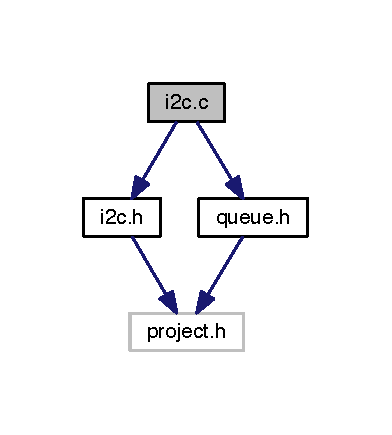
\includegraphics[width=350pt]{d6/d4e/i2c_8c__incl}
\end{center}
\end{figure}


\subsubsection{Detaljeret beskrivelse}
\hyperlink{class_i2_c}{I2C} modul. 

Håndter kommunikation via I2\+C-\/busset \begin{DoxyAuthor}{Forfatter}
Jeppe Stærk Antonsen (\href{mailto:201271201@uni.au.dk}{\tt 201271201@uni.\+au.\+dk}) 
\end{DoxyAuthor}

\hypertarget{i2c_8h}{}\subsection{i2c.\+h filreference}
\label{i2c_8h}\index{i2c.\+h@{i2c.\+h}}


\hyperlink{class_i2_c}{I2C} modul.  


{\ttfamily \#include $<$project.\+h$>$}\\*
Inklusions-\/afhængighedsgraf for i2c.\+h\+:\nopagebreak
\begin{figure}[H]
\begin{center}
\leavevmode
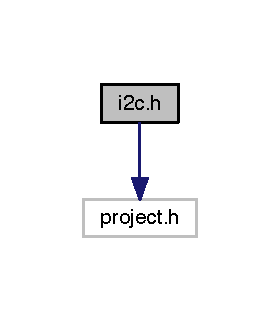
\includegraphics[width=134pt]{de/d0d/i2c_8h__incl}
\end{center}
\end{figure}
Denne graf viser, hvilke filer der direkte eller indirekte inkluderer denne fil\+:\nopagebreak
\begin{figure}[H]
\begin{center}
\leavevmode
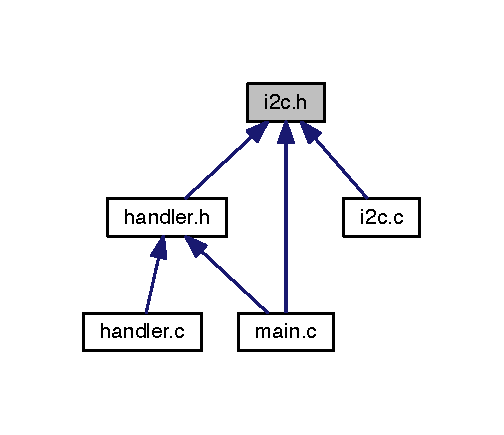
\includegraphics[width=255pt]{d3/df7/i2c_8h__dep__incl}
\end{center}
\end{figure}
\subsubsection*{\#Defines}
\begin{DoxyCompactItemize}
\item 
\#define \hyperlink{i2c_8h_a2c70db7df8defae29c1912d84aaee3dc}{P\+So\+C\+\_\+\+XY}~(0x08u)
\item 
\#define \hyperlink{i2c_8h_aa72315d85eb390444fdd96475c6aa1f4}{P\+So\+C\+\_\+Z}~(0x09u)
\item 
\#define \hyperlink{i2c_8h_adc44ca05813864518773ea6f3543816c}{P\+So\+C\+\_\+\+Sensor}~(0x10u)
\item 
\#define \hyperlink{i2c_8h_a6458dbf193a0eef0470fc1b08400bfcd}{I2\+C\+\_\+\+B\+U\+F\+F\+E\+R\+\_\+\+S\+I\+ZE}~(4u)
\item 
\#define \hyperlink{i2c_8h_a8c24abf58121f3c16b5f687cc2946cd1}{I2\+C\+\_\+\+P\+A\+C\+K\+E\+T\+\_\+\+S\+I\+ZE}~(4u)
\item 
\#define \hyperlink{i2c_8h_a1207f4b2c3692b1a344f0013da629310}{I2\+C\+\_\+\+P\+A\+C\+K\+E\+T\+\_\+\+S\+O\+P\+\_\+\+P\+OS}~(0u)
\item 
\#define \hyperlink{i2c_8h_ac13fcfeded7dc2d82fa4734456f3761f}{I2\+C\+\_\+\+P\+A\+C\+K\+E\+T\+\_\+\+C\+M\+D\+\_\+\+P\+OS}~(1u)
\item 
\#define \hyperlink{i2c_8h_a68506c3651f015716bb2c135e8e7b972}{I2\+C\+\_\+\+P\+A\+C\+K\+E\+T\+\_\+\+V\+A\+L\+\_\+\+P\+OS}~(2u)
\item 
\#define \hyperlink{i2c_8h_a940f0ea8103872c7ba81b9dc0f121feb}{I2\+C\+\_\+\+P\+A\+C\+K\+E\+T\+\_\+\+E\+O\+P\+\_\+\+P\+OS}~(3u)
\item 
\#define \hyperlink{i2c_8h_a52bb5b964361ed2f1b18df32c5b8f2c5}{I2\+C\+\_\+\+P\+A\+C\+K\+E\+T\+\_\+\+S\+OP}~(0x\+B\+Eu)
\item 
\#define \hyperlink{i2c_8h_a62b4ae6e51a3d0da47f5165165cdbc0a}{I2\+C\+\_\+\+P\+A\+C\+K\+E\+T\+\_\+\+E\+OP}~(0x\+E\+Fu)
\item 
\#define \hyperlink{i2c_8h_a7f8f53679384fa228bf06779cc168cfd}{I2\+C\+\_\+\+S\+T\+S\+\_\+\+C\+M\+D\+\_\+\+D\+O\+NE}~(0x\+A\+Au)
\item 
\#define \hyperlink{i2c_8h_aee0adbd7dcb13e95337369b7342a27e3}{I2\+C\+\_\+\+S\+T\+S\+\_\+\+C\+M\+D\+\_\+\+F\+A\+IL}~(0x\+E\+Eu)
\end{DoxyCompactItemize}
\subsubsection*{Funktioner}
\begin{DoxyCompactItemize}
\item 
void \hyperlink{i2c_8h_a5730d9445429351b9f750084c5cb5aae}{i2c\+\_\+init} (void)
\item 
void \hyperlink{i2c_8h_a0e13c9c7d87ebdb3680495a787f68d29}{i2c\+\_\+set\+Packet} (uint8 i2c\+Addr, uint8 i2c\+Cmd, uint8 i2c\+Val)
\item 
void \hyperlink{i2c_8h_afd44ef28b428b7ec2cffb38c97340251}{i2c\+\_\+get\+Packet} (uint8 i2c\+Addr, uint8 i2c\+Cmd, uint8 $\ast$i2c\+Val)
\end{DoxyCompactItemize}


\subsubsection{Detaljeret beskrivelse}
\hyperlink{class_i2_c}{I2C} modul. 

Håndter kommunikation via I2\+C-\/busset. \begin{DoxyAuthor}{Forfatter}
Jeppe Stærk Antonsen (\href{mailto:201271201@uni.au.dk}{\tt 201271201@uni.\+au.\+dk}) 
\end{DoxyAuthor}


\subsubsection{\#Define-\/dokumentation}
\index{i2c.\+h@{i2c.\+h}!I2\+C\+\_\+\+B\+U\+F\+F\+E\+R\+\_\+\+S\+I\+ZE@{I2\+C\+\_\+\+B\+U\+F\+F\+E\+R\+\_\+\+S\+I\+ZE}}
\index{I2\+C\+\_\+\+B\+U\+F\+F\+E\+R\+\_\+\+S\+I\+ZE@{I2\+C\+\_\+\+B\+U\+F\+F\+E\+R\+\_\+\+S\+I\+ZE}!i2c.\+h@{i2c.\+h}}
\paragraph[{\texorpdfstring{I2\+C\+\_\+\+B\+U\+F\+F\+E\+R\+\_\+\+S\+I\+ZE}{I2C_BUFFER_SIZE}}]{\setlength{\rightskip}{0pt plus 5cm}\#define I2\+C\+\_\+\+B\+U\+F\+F\+E\+R\+\_\+\+S\+I\+ZE~(4u)}\hypertarget{i2c_8h_a6458dbf193a0eef0470fc1b08400bfcd}{}\label{i2c_8h_a6458dbf193a0eef0470fc1b08400bfcd}


Defineret på linje 42 i filen i2c.\+h.



Refereret til af I2\+C\+::i2c\+\_\+rx() og I2\+C\+::i2c\+\_\+tx().

\index{i2c.\+h@{i2c.\+h}!I2\+C\+\_\+\+P\+A\+C\+K\+E\+T\+\_\+\+C\+M\+D\+\_\+\+P\+OS@{I2\+C\+\_\+\+P\+A\+C\+K\+E\+T\+\_\+\+C\+M\+D\+\_\+\+P\+OS}}
\index{I2\+C\+\_\+\+P\+A\+C\+K\+E\+T\+\_\+\+C\+M\+D\+\_\+\+P\+OS@{I2\+C\+\_\+\+P\+A\+C\+K\+E\+T\+\_\+\+C\+M\+D\+\_\+\+P\+OS}!i2c.\+h@{i2c.\+h}}
\paragraph[{\texorpdfstring{I2\+C\+\_\+\+P\+A\+C\+K\+E\+T\+\_\+\+C\+M\+D\+\_\+\+P\+OS}{I2C_PACKET_CMD_POS}}]{\setlength{\rightskip}{0pt plus 5cm}\#define I2\+C\+\_\+\+P\+A\+C\+K\+E\+T\+\_\+\+C\+M\+D\+\_\+\+P\+OS~(1u)}\hypertarget{i2c_8h_ac13fcfeded7dc2d82fa4734456f3761f}{}\label{i2c_8h_ac13fcfeded7dc2d82fa4734456f3761f}


Defineret på linje 47 i filen i2c.\+h.



Refereret til af I2\+C\+::i2c\+\_\+rx() og I2\+C\+::i2c\+\_\+tx().

\index{i2c.\+h@{i2c.\+h}!I2\+C\+\_\+\+P\+A\+C\+K\+E\+T\+\_\+\+E\+OP@{I2\+C\+\_\+\+P\+A\+C\+K\+E\+T\+\_\+\+E\+OP}}
\index{I2\+C\+\_\+\+P\+A\+C\+K\+E\+T\+\_\+\+E\+OP@{I2\+C\+\_\+\+P\+A\+C\+K\+E\+T\+\_\+\+E\+OP}!i2c.\+h@{i2c.\+h}}
\paragraph[{\texorpdfstring{I2\+C\+\_\+\+P\+A\+C\+K\+E\+T\+\_\+\+E\+OP}{I2C_PACKET_EOP}}]{\setlength{\rightskip}{0pt plus 5cm}\#define I2\+C\+\_\+\+P\+A\+C\+K\+E\+T\+\_\+\+E\+OP~(0x\+E\+Fu)}\hypertarget{i2c_8h_a62b4ae6e51a3d0da47f5165165cdbc0a}{}\label{i2c_8h_a62b4ae6e51a3d0da47f5165165cdbc0a}


Defineret på linje 53 i filen i2c.\+h.



Refereret til af I2\+C\+::i2c\+\_\+rx() og I2\+C\+::i2c\+\_\+tx().

\index{i2c.\+h@{i2c.\+h}!I2\+C\+\_\+\+P\+A\+C\+K\+E\+T\+\_\+\+E\+O\+P\+\_\+\+P\+OS@{I2\+C\+\_\+\+P\+A\+C\+K\+E\+T\+\_\+\+E\+O\+P\+\_\+\+P\+OS}}
\index{I2\+C\+\_\+\+P\+A\+C\+K\+E\+T\+\_\+\+E\+O\+P\+\_\+\+P\+OS@{I2\+C\+\_\+\+P\+A\+C\+K\+E\+T\+\_\+\+E\+O\+P\+\_\+\+P\+OS}!i2c.\+h@{i2c.\+h}}
\paragraph[{\texorpdfstring{I2\+C\+\_\+\+P\+A\+C\+K\+E\+T\+\_\+\+E\+O\+P\+\_\+\+P\+OS}{I2C_PACKET_EOP_POS}}]{\setlength{\rightskip}{0pt plus 5cm}\#define I2\+C\+\_\+\+P\+A\+C\+K\+E\+T\+\_\+\+E\+O\+P\+\_\+\+P\+OS~(3u)}\hypertarget{i2c_8h_a940f0ea8103872c7ba81b9dc0f121feb}{}\label{i2c_8h_a940f0ea8103872c7ba81b9dc0f121feb}


Defineret på linje 49 i filen i2c.\+h.



Refereret til af I2\+C\+::i2c\+\_\+rx() og I2\+C\+::i2c\+\_\+tx().

\index{i2c.\+h@{i2c.\+h}!I2\+C\+\_\+\+P\+A\+C\+K\+E\+T\+\_\+\+S\+I\+ZE@{I2\+C\+\_\+\+P\+A\+C\+K\+E\+T\+\_\+\+S\+I\+ZE}}
\index{I2\+C\+\_\+\+P\+A\+C\+K\+E\+T\+\_\+\+S\+I\+ZE@{I2\+C\+\_\+\+P\+A\+C\+K\+E\+T\+\_\+\+S\+I\+ZE}!i2c.\+h@{i2c.\+h}}
\paragraph[{\texorpdfstring{I2\+C\+\_\+\+P\+A\+C\+K\+E\+T\+\_\+\+S\+I\+ZE}{I2C_PACKET_SIZE}}]{\setlength{\rightskip}{0pt plus 5cm}\#define I2\+C\+\_\+\+P\+A\+C\+K\+E\+T\+\_\+\+S\+I\+ZE~(4u)}\hypertarget{i2c_8h_a8c24abf58121f3c16b5f687cc2946cd1}{}\label{i2c_8h_a8c24abf58121f3c16b5f687cc2946cd1}


Defineret på linje 43 i filen i2c.\+h.



Refereret til af I2\+C\+::i2c\+\_\+rx() og I2\+C\+::i2c\+\_\+tx().

\index{i2c.\+h@{i2c.\+h}!I2\+C\+\_\+\+P\+A\+C\+K\+E\+T\+\_\+\+S\+OP@{I2\+C\+\_\+\+P\+A\+C\+K\+E\+T\+\_\+\+S\+OP}}
\index{I2\+C\+\_\+\+P\+A\+C\+K\+E\+T\+\_\+\+S\+OP@{I2\+C\+\_\+\+P\+A\+C\+K\+E\+T\+\_\+\+S\+OP}!i2c.\+h@{i2c.\+h}}
\paragraph[{\texorpdfstring{I2\+C\+\_\+\+P\+A\+C\+K\+E\+T\+\_\+\+S\+OP}{I2C_PACKET_SOP}}]{\setlength{\rightskip}{0pt plus 5cm}\#define I2\+C\+\_\+\+P\+A\+C\+K\+E\+T\+\_\+\+S\+OP~(0x\+B\+Eu)}\hypertarget{i2c_8h_a52bb5b964361ed2f1b18df32c5b8f2c5}{}\label{i2c_8h_a52bb5b964361ed2f1b18df32c5b8f2c5}


Defineret på linje 52 i filen i2c.\+h.



Refereret til af I2\+C\+::i2c\+\_\+rx() og I2\+C\+::i2c\+\_\+tx().

\index{i2c.\+h@{i2c.\+h}!I2\+C\+\_\+\+P\+A\+C\+K\+E\+T\+\_\+\+S\+O\+P\+\_\+\+P\+OS@{I2\+C\+\_\+\+P\+A\+C\+K\+E\+T\+\_\+\+S\+O\+P\+\_\+\+P\+OS}}
\index{I2\+C\+\_\+\+P\+A\+C\+K\+E\+T\+\_\+\+S\+O\+P\+\_\+\+P\+OS@{I2\+C\+\_\+\+P\+A\+C\+K\+E\+T\+\_\+\+S\+O\+P\+\_\+\+P\+OS}!i2c.\+h@{i2c.\+h}}
\paragraph[{\texorpdfstring{I2\+C\+\_\+\+P\+A\+C\+K\+E\+T\+\_\+\+S\+O\+P\+\_\+\+P\+OS}{I2C_PACKET_SOP_POS}}]{\setlength{\rightskip}{0pt plus 5cm}\#define I2\+C\+\_\+\+P\+A\+C\+K\+E\+T\+\_\+\+S\+O\+P\+\_\+\+P\+OS~(0u)}\hypertarget{i2c_8h_a1207f4b2c3692b1a344f0013da629310}{}\label{i2c_8h_a1207f4b2c3692b1a344f0013da629310}


Defineret på linje 46 i filen i2c.\+h.



Refereret til af I2\+C\+::i2c\+\_\+rx() og I2\+C\+::i2c\+\_\+tx().

\index{i2c.\+h@{i2c.\+h}!I2\+C\+\_\+\+P\+A\+C\+K\+E\+T\+\_\+\+V\+A\+L\+\_\+\+P\+OS@{I2\+C\+\_\+\+P\+A\+C\+K\+E\+T\+\_\+\+V\+A\+L\+\_\+\+P\+OS}}
\index{I2\+C\+\_\+\+P\+A\+C\+K\+E\+T\+\_\+\+V\+A\+L\+\_\+\+P\+OS@{I2\+C\+\_\+\+P\+A\+C\+K\+E\+T\+\_\+\+V\+A\+L\+\_\+\+P\+OS}!i2c.\+h@{i2c.\+h}}
\paragraph[{\texorpdfstring{I2\+C\+\_\+\+P\+A\+C\+K\+E\+T\+\_\+\+V\+A\+L\+\_\+\+P\+OS}{I2C_PACKET_VAL_POS}}]{\setlength{\rightskip}{0pt plus 5cm}\#define I2\+C\+\_\+\+P\+A\+C\+K\+E\+T\+\_\+\+V\+A\+L\+\_\+\+P\+OS~(2u)}\hypertarget{i2c_8h_a68506c3651f015716bb2c135e8e7b972}{}\label{i2c_8h_a68506c3651f015716bb2c135e8e7b972}


Defineret på linje 48 i filen i2c.\+h.



Refereret til af I2\+C\+::i2c\+\_\+rx() og I2\+C\+::i2c\+\_\+tx().

\index{i2c.\+h@{i2c.\+h}!I2\+C\+\_\+\+S\+T\+S\+\_\+\+C\+M\+D\+\_\+\+D\+O\+NE@{I2\+C\+\_\+\+S\+T\+S\+\_\+\+C\+M\+D\+\_\+\+D\+O\+NE}}
\index{I2\+C\+\_\+\+S\+T\+S\+\_\+\+C\+M\+D\+\_\+\+D\+O\+NE@{I2\+C\+\_\+\+S\+T\+S\+\_\+\+C\+M\+D\+\_\+\+D\+O\+NE}!i2c.\+h@{i2c.\+h}}
\paragraph[{\texorpdfstring{I2\+C\+\_\+\+S\+T\+S\+\_\+\+C\+M\+D\+\_\+\+D\+O\+NE}{I2C_STS_CMD_DONE}}]{\setlength{\rightskip}{0pt plus 5cm}\#define I2\+C\+\_\+\+S\+T\+S\+\_\+\+C\+M\+D\+\_\+\+D\+O\+NE~(0x\+A\+Au)}\hypertarget{i2c_8h_a7f8f53679384fa228bf06779cc168cfd}{}\label{i2c_8h_a7f8f53679384fa228bf06779cc168cfd}


Defineret på linje 56 i filen i2c.\+h.



Refereret til af I2\+C\+::i2c\+\_\+get\+Packet(), I2\+C\+::i2c\+\_\+set\+Packet() og I2\+C\+::i2c\+\_\+tx().

\index{i2c.\+h@{i2c.\+h}!I2\+C\+\_\+\+S\+T\+S\+\_\+\+C\+M\+D\+\_\+\+F\+A\+IL@{I2\+C\+\_\+\+S\+T\+S\+\_\+\+C\+M\+D\+\_\+\+F\+A\+IL}}
\index{I2\+C\+\_\+\+S\+T\+S\+\_\+\+C\+M\+D\+\_\+\+F\+A\+IL@{I2\+C\+\_\+\+S\+T\+S\+\_\+\+C\+M\+D\+\_\+\+F\+A\+IL}!i2c.\+h@{i2c.\+h}}
\paragraph[{\texorpdfstring{I2\+C\+\_\+\+S\+T\+S\+\_\+\+C\+M\+D\+\_\+\+F\+A\+IL}{I2C_STS_CMD_FAIL}}]{\setlength{\rightskip}{0pt plus 5cm}\#define I2\+C\+\_\+\+S\+T\+S\+\_\+\+C\+M\+D\+\_\+\+F\+A\+IL~(0x\+E\+Eu)}\hypertarget{i2c_8h_aee0adbd7dcb13e95337369b7342a27e3}{}\label{i2c_8h_aee0adbd7dcb13e95337369b7342a27e3}


Defineret på linje 57 i filen i2c.\+h.



Refereret til af I2\+C\+::i2c\+\_\+rx() og I2\+C\+::i2c\+\_\+tx().

\index{i2c.\+h@{i2c.\+h}!P\+So\+C\+\_\+\+Sensor@{P\+So\+C\+\_\+\+Sensor}}
\index{P\+So\+C\+\_\+\+Sensor@{P\+So\+C\+\_\+\+Sensor}!i2c.\+h@{i2c.\+h}}
\paragraph[{\texorpdfstring{P\+So\+C\+\_\+\+Sensor}{PSoC_Sensor}}]{\setlength{\rightskip}{0pt plus 5cm}\#define P\+So\+C\+\_\+\+Sensor~(0x10u)}\hypertarget{i2c_8h_adc44ca05813864518773ea6f3543816c}{}\label{i2c_8h_adc44ca05813864518773ea6f3543816c}


Defineret på linje 39 i filen i2c.\+h.



Refereret til af Handler\+::handler().

\index{i2c.\+h@{i2c.\+h}!P\+So\+C\+\_\+\+XY@{P\+So\+C\+\_\+\+XY}}
\index{P\+So\+C\+\_\+\+XY@{P\+So\+C\+\_\+\+XY}!i2c.\+h@{i2c.\+h}}
\paragraph[{\texorpdfstring{P\+So\+C\+\_\+\+XY}{PSoC_XY}}]{\setlength{\rightskip}{0pt plus 5cm}\#define P\+So\+C\+\_\+\+XY~(0x08u)}\hypertarget{i2c_8h_a2c70db7df8defae29c1912d84aaee3dc}{}\label{i2c_8h_a2c70db7df8defae29c1912d84aaee3dc}


Defineret på linje 37 i filen i2c.\+h.



Refereret til af Handler\+::handler().

\index{i2c.\+h@{i2c.\+h}!P\+So\+C\+\_\+Z@{P\+So\+C\+\_\+Z}}
\index{P\+So\+C\+\_\+Z@{P\+So\+C\+\_\+Z}!i2c.\+h@{i2c.\+h}}
\paragraph[{\texorpdfstring{P\+So\+C\+\_\+Z}{PSoC_Z}}]{\setlength{\rightskip}{0pt plus 5cm}\#define P\+So\+C\+\_\+Z~(0x09u)}\hypertarget{i2c_8h_aa72315d85eb390444fdd96475c6aa1f4}{}\label{i2c_8h_aa72315d85eb390444fdd96475c6aa1f4}


Defineret på linje 38 i filen i2c.\+h.



Refereret til af Handler\+::handler().



\subsubsection{Funktions-\/dokumentation}
\index{i2c.\+h@{i2c.\+h}!i2c\+\_\+get\+Packet@{i2c\+\_\+get\+Packet}}
\index{i2c\+\_\+get\+Packet@{i2c\+\_\+get\+Packet}!i2c.\+h@{i2c.\+h}}
\paragraph[{\texorpdfstring{i2c\+\_\+get\+Packet(uint8 i2c\+Addr, uint8 i2c\+Cmd, uint8 $\ast$i2c\+Val)}{i2c_getPacket(uint8 i2cAddr, uint8 i2cCmd, uint8 *i2cVal)}}]{\setlength{\rightskip}{0pt plus 5cm}void i2c\+\_\+get\+Packet (
\begin{DoxyParamCaption}
\item[{uint8}]{i2c\+Addr, }
\item[{uint8}]{i2c\+Cmd, }
\item[{uint8 $\ast$}]{i2c\+Val}
\end{DoxyParamCaption}
)}\hypertarget{i2c_8h_afd44ef28b428b7ec2cffb38c97340251}{}\label{i2c_8h_afd44ef28b428b7ec2cffb38c97340251}
\index{i2c.\+h@{i2c.\+h}!i2c\+\_\+init@{i2c\+\_\+init}}
\index{i2c\+\_\+init@{i2c\+\_\+init}!i2c.\+h@{i2c.\+h}}
\paragraph[{\texorpdfstring{i2c\+\_\+init(void)}{i2c_init(void)}}]{\setlength{\rightskip}{0pt plus 5cm}void i2c\+\_\+init (
\begin{DoxyParamCaption}
\item[{void}]{}
\end{DoxyParamCaption}
)}\hypertarget{i2c_8h_a5730d9445429351b9f750084c5cb5aae}{}\label{i2c_8h_a5730d9445429351b9f750084c5cb5aae}
\index{i2c.\+h@{i2c.\+h}!i2c\+\_\+set\+Packet@{i2c\+\_\+set\+Packet}}
\index{i2c\+\_\+set\+Packet@{i2c\+\_\+set\+Packet}!i2c.\+h@{i2c.\+h}}
\paragraph[{\texorpdfstring{i2c\+\_\+set\+Packet(uint8 i2c\+Addr, uint8 i2c\+Cmd, uint8 i2c\+Val)}{i2c_setPacket(uint8 i2cAddr, uint8 i2cCmd, uint8 i2cVal)}}]{\setlength{\rightskip}{0pt plus 5cm}void i2c\+\_\+set\+Packet (
\begin{DoxyParamCaption}
\item[{uint8}]{i2c\+Addr, }
\item[{uint8}]{i2c\+Cmd, }
\item[{uint8}]{i2c\+Val}
\end{DoxyParamCaption}
)}\hypertarget{i2c_8h_a0e13c9c7d87ebdb3680495a787f68d29}{}\label{i2c_8h_a0e13c9c7d87ebdb3680495a787f68d29}

\hypertarget{_lumen_sensor_8c}{}\subsection{Lumen\+Sensor.\+c filreference}
\label{_lumen_sensor_8c}\index{Lumen\+Sensor.\+c@{Lumen\+Sensor.\+c}}


Handles the light sensor. Both initialization and data extraction.  


{\ttfamily \#include \char`\"{}Lumen\+Sensor.\+h\char`\"{}}\\*
{\ttfamily \#include \char`\"{}lux.\+h\char`\"{}}\\*
{\ttfamily \#include \char`\"{}Sensor\+Data.\+h\char`\"{}}\\*
Inklusions-\/afhængighedsgraf for Lumen\+Sensor.\+c\+:\nopagebreak
\begin{figure}[H]
\begin{center}
\leavevmode
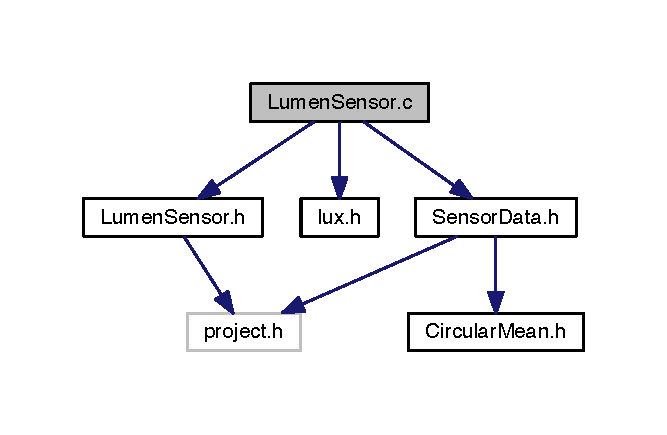
\includegraphics[width=320pt]{d1/db0/_lumen_sensor_8c__incl}
\end{center}
\end{figure}
\subsubsection*{\#Defines}
\begin{DoxyCompactItemize}
\item 
\#define \hyperlink{_lumen_sensor_8c_aee9d6665305479ca38bc745e6f09a336}{L\+U\+M\+E\+N\+\_\+\+A\+D\+DR}~0b0101001
\end{DoxyCompactItemize}
\subsubsection*{Funktioner}
\begin{DoxyCompactItemize}
\item 
void \hyperlink{_lumen_sensor_8c_a89993394d4ef10fb5362c18ab189ad31}{init\+Lumen\+Sensor} ()
\begin{DoxyCompactList}\small\item\em Initialize the light sensor. \end{DoxyCompactList}\item 
unsigned int \hyperlink{_lumen_sensor_8c_acbfb15efe3f5e10e4de610ba5e3ef9e7}{read\+Lumen\+Sensor} ()
\begin{DoxyCompactList}\small\item\em Read sensor data from the light sensor. \end{DoxyCompactList}\item 
uint8 \hyperlink{_lumen_sensor_8c_a1337221b40e407eeb46861aef99c6b83}{scale\+Lux\+To\+FF} (unsigned int val)
\begin{DoxyCompactList}\small\item\em Scale a lux value into a 0-\/255 range value Due to the limited range to scale into, lux over 1530 is scaled to 255. The top 1530 vas chosen because 1530/255 = 6. \end{DoxyCompactList}\item 
unsigned int \hyperlink{_lumen_sensor_8c_a4e19311d2241c61d7b3a7ca9cd5fb765}{scale\+F\+Fto\+Lux} (uint8 val)
\begin{DoxyCompactList}\small\item\em Scale a 0-\/255 range value into lux Due to the limited input range 1530 has been chosen as max value for lux. The top 1530 vas chosen because 1530/255 = 6. \end{DoxyCompactList}\end{DoxyCompactItemize}


\subsubsection{Detaljeret beskrivelse}
Handles the light sensor. Both initialization and data extraction. 

\begin{DoxyAuthor}{Forfatter}
Simon Nejmann (\href{mailto:19981127@uni.au.dk}{\tt 19981127@uni.\+au.\+dk}) 
\end{DoxyAuthor}


\subsubsection{\#Define-\/dokumentation}
\index{Lumen\+Sensor.\+c@{Lumen\+Sensor.\+c}!L\+U\+M\+E\+N\+\_\+\+A\+D\+DR@{L\+U\+M\+E\+N\+\_\+\+A\+D\+DR}}
\index{L\+U\+M\+E\+N\+\_\+\+A\+D\+DR@{L\+U\+M\+E\+N\+\_\+\+A\+D\+DR}!Lumen\+Sensor.\+c@{Lumen\+Sensor.\+c}}
\paragraph[{\texorpdfstring{L\+U\+M\+E\+N\+\_\+\+A\+D\+DR}{LUMEN_ADDR}}]{\setlength{\rightskip}{0pt plus 5cm}\#define L\+U\+M\+E\+N\+\_\+\+A\+D\+DR~0b0101001}\hypertarget{_lumen_sensor_8c_aee9d6665305479ca38bc745e6f09a336}{}\label{_lumen_sensor_8c_aee9d6665305479ca38bc745e6f09a336}
The I2C address of the light sensor 

Defineret på linje 11 i filen Lumen\+Sensor.\+c.



Refereret til af init\+Lumen\+Sensor() og read\+Lumen\+Sensor().



\subsubsection{Funktions-\/dokumentation}
\index{Lumen\+Sensor.\+c@{Lumen\+Sensor.\+c}!init\+Lumen\+Sensor@{init\+Lumen\+Sensor}}
\index{init\+Lumen\+Sensor@{init\+Lumen\+Sensor}!Lumen\+Sensor.\+c@{Lumen\+Sensor.\+c}}
\paragraph[{\texorpdfstring{init\+Lumen\+Sensor()}{initLumenSensor()}}]{\setlength{\rightskip}{0pt plus 5cm}void init\+Lumen\+Sensor (
\begin{DoxyParamCaption}
{}
\end{DoxyParamCaption}
)}\hypertarget{_lumen_sensor_8c_a89993394d4ef10fb5362c18ab189ad31}{}\label{_lumen_sensor_8c_a89993394d4ef10fb5362c18ab189ad31}


Initialize the light sensor. 

\begin{DoxyAuthor}{Forfatter}
Simon Nejmann (\href{mailto:19981127@uni.au.dk}{\tt 19981127@uni.\+au.\+dk}) 
\end{DoxyAuthor}


Defineret på linje 18 i filen Lumen\+Sensor.\+c.



Indeholder referencer til L\+U\+M\+E\+N\+\_\+\+A\+D\+DR.



Refereret til af main().


\begin{DoxyCode}
19 \{
20     uint8 writeBuf[2];
21     uint32 err;
22     
23     \textcolor{comment}{// Add internal pull-up resistors on the SCL and SDA lines}
24     LumenCom\_scl\_SetDriveMode(LumenCom\_scl\_DM\_RES\_UP);
25     LumenCom\_sda\_SetDriveMode(LumenCom\_sda\_DM\_RES\_UP);
26 
27     LumenCom\_Start();
28     \textcolor{comment}{// Send command to sensor:}
29     writeBuf[0] = 0x80; \textcolor{comment}{// Highest bit set = command, low bits 0000 = control register}
30     writeBuf[1] = 0x03; \textcolor{comment}{// Power up sensor}
31     err = LumenCom\_I2CMasterWriteBuf(\hyperlink{_lumen_sensor_8c_aee9d6665305479ca38bc745e6f09a336}{LUMEN\_ADDR}, writeBuf, 2, LumenCom\_I2C\_MODE\_COMPLETE\_XFER);
32     \textcolor{comment}{// Wait for the I2C command to finish transferring:}
33     \textcolor{keywordflow}{while}(LumenCom\_I2CMasterStatus() & LumenCom\_I2C\_MSTAT\_XFER\_INP) \{\}
34 \}
\end{DoxyCode}


Her er kalder-\/grafen for denne funktion\+:\nopagebreak
\begin{figure}[H]
\begin{center}
\leavevmode
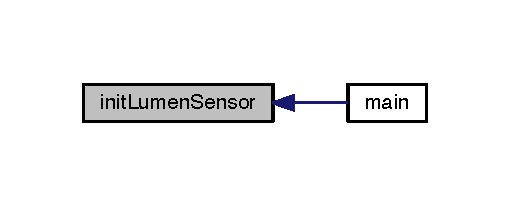
\includegraphics[width=245pt]{db/d85/_lumen_sensor_8c_a89993394d4ef10fb5362c18ab189ad31_icgraph}
\end{center}
\end{figure}


\index{Lumen\+Sensor.\+c@{Lumen\+Sensor.\+c}!read\+Lumen\+Sensor@{read\+Lumen\+Sensor}}
\index{read\+Lumen\+Sensor@{read\+Lumen\+Sensor}!Lumen\+Sensor.\+c@{Lumen\+Sensor.\+c}}
\paragraph[{\texorpdfstring{read\+Lumen\+Sensor()}{readLumenSensor()}}]{\setlength{\rightskip}{0pt plus 5cm}unsigned int read\+Lumen\+Sensor (
\begin{DoxyParamCaption}
{}
\end{DoxyParamCaption}
)}\hypertarget{_lumen_sensor_8c_acbfb15efe3f5e10e4de610ba5e3ef9e7}{}\label{_lumen_sensor_8c_acbfb15efe3f5e10e4de610ba5e3ef9e7}


Read sensor data from the light sensor. 

\begin{DoxyReturn}{Returnerer}
The lux value of the perceived light
\end{DoxyReturn}
\begin{DoxyAuthor}{Forfatter}
Simon Nejmann (\href{mailto:19981127@uni.au.dk}{\tt 19981127@uni.\+au.\+dk}) 
\end{DoxyAuthor}


Defineret på linje 42 i filen Lumen\+Sensor.\+c.



Indeholder referencer til Calculate\+Lux() og L\+U\+M\+E\+N\+\_\+\+A\+D\+DR.



Refereret til af main().


\begin{DoxyCode}
43 \{
44     uint8 readBuf[2];
45     uint8 writeBuf[1];
46     \textcolor{keywordtype}{unsigned} \textcolor{keywordtype}{int} channel0 = 0;
47     \textcolor{keywordtype}{unsigned} \textcolor{keywordtype}{int} channel1 = 0;
48 
49     \textcolor{comment}{// Send "read channel 0" command}
50     writeBuf[0] = 0xAC;
51     LumenCom\_I2CMasterWriteBuf(\hyperlink{_lumen_sensor_8c_aee9d6665305479ca38bc745e6f09a336}{LUMEN\_ADDR}, writeBuf, 1, LumenCom\_I2C\_MODE\_NO\_STOP);
52 
53     \textcolor{comment}{// Wait for the I2C command to finish transferring}
54     \textcolor{keywordflow}{while}(!(LumenCom\_I2CMasterStatus() & LumenCom\_I2C\_MSTAT\_XFER\_HALT)) \{\}
55     \textcolor{comment}{// Read two bytes of data}
56     LumenCom\_I2CMasterReadBuf(\hyperlink{_lumen_sensor_8c_aee9d6665305479ca38bc745e6f09a336}{LUMEN\_ADDR}, readBuf, 2,
57         LumenCom\_I2C\_MODE\_REPEAT\_START | LumenCom\_I2C\_MODE\_NO\_STOP);
58 
59     \textcolor{comment}{// Wait for the I2C command to finish transferring}
60     \textcolor{keywordflow}{while}(!(LumenCom\_I2CMasterStatus() & LumenCom\_I2C\_MSTAT\_XFER\_HALT)) \{\}
61 
62     channel0 = readBuf[0] + readBuf[1] * 256;
63 
64     \textcolor{comment}{// Send "read channel 1" command}
65     writeBuf[0] = 0xAE;
66     LumenCom\_I2CMasterWriteBuf(\hyperlink{_lumen_sensor_8c_aee9d6665305479ca38bc745e6f09a336}{LUMEN\_ADDR}, writeBuf, 1,
67         LumenCom\_I2C\_MODE\_REPEAT\_START | LumenCom\_I2C\_MODE\_NO\_STOP);
68 
69     \textcolor{comment}{// Wait for the I2C command to finish transferring}
70     \textcolor{keywordflow}{while}(!(LumenCom\_I2CMasterStatus() & LumenCom\_I2C\_MSTAT\_XFER\_HALT)) \{\}
71     \textcolor{comment}{// Read two bytes of data}
72     LumenCom\_I2CMasterReadBuf(\hyperlink{_lumen_sensor_8c_aee9d6665305479ca38bc745e6f09a336}{LUMEN\_ADDR}, readBuf, 2, LumenCom\_I2C\_MODE\_REPEAT\_START);
73 
74     \textcolor{comment}{// Wait for the I2C command to finish transferring}
75     \textcolor{keywordflow}{while}(LumenCom\_I2CMasterStatus() & LumenCom\_I2C\_MSTAT\_XFER\_INP) \{\}
76 
77     channel1 = readBuf[0] + readBuf[1] * 256;
78 
79     \textcolor{comment}{// Use Datasheet function to calculate lux value from read values}
80     \textcolor{keywordflow}{return} \hyperlink{lux_8c_a3db2aa0d603f0627be256dc108d3d763}{CalculateLux}(0, 2, channel0, channel1, 0);
81 \}
\end{DoxyCode}


Her er kald-\/grafen for denne funktion\+:\nopagebreak
\begin{figure}[H]
\begin{center}
\leavevmode
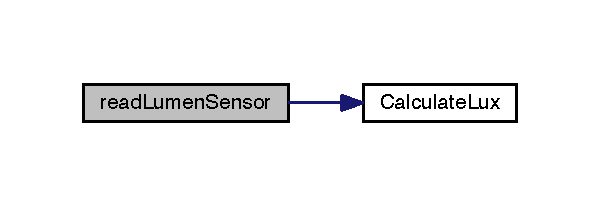
\includegraphics[width=288pt]{db/d85/_lumen_sensor_8c_acbfb15efe3f5e10e4de610ba5e3ef9e7_cgraph}
\end{center}
\end{figure}




Her er kalder-\/grafen for denne funktion\+:\nopagebreak
\begin{figure}[H]
\begin{center}
\leavevmode
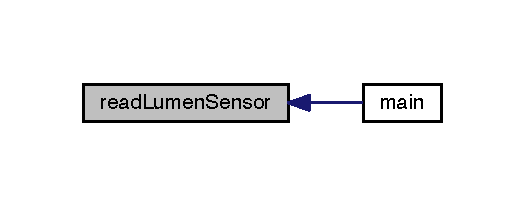
\includegraphics[width=252pt]{db/d85/_lumen_sensor_8c_acbfb15efe3f5e10e4de610ba5e3ef9e7_icgraph}
\end{center}
\end{figure}


\index{Lumen\+Sensor.\+c@{Lumen\+Sensor.\+c}!scale\+F\+Fto\+Lux@{scale\+F\+Fto\+Lux}}
\index{scale\+F\+Fto\+Lux@{scale\+F\+Fto\+Lux}!Lumen\+Sensor.\+c@{Lumen\+Sensor.\+c}}
\paragraph[{\texorpdfstring{scale\+F\+Fto\+Lux(uint8 val)}{scaleFFtoLux(uint8 val)}}]{\setlength{\rightskip}{0pt plus 5cm}unsigned int scale\+F\+Fto\+Lux (
\begin{DoxyParamCaption}
\item[{uint8}]{val}
\end{DoxyParamCaption}
)}\hypertarget{_lumen_sensor_8c_a4e19311d2241c61d7b3a7ca9cd5fb765}{}\label{_lumen_sensor_8c_a4e19311d2241c61d7b3a7ca9cd5fb765}


Scale a 0-\/255 range value into lux Due to the limited input range 1530 has been chosen as max value for lux. The top 1530 vas chosen because 1530/255 = 6. 

\begin{DoxyReturn}{Returnerer}
The an upscaled lux value 
\end{DoxyReturn}

\begin{DoxyParams}[1]{Parametre}
\mbox{\tt in}  & {\em val} & uint8 containing a value to scale up\\
\hline
\end{DoxyParams}
\begin{DoxyAuthor}{Forfatter}
Simon Nejmann (\href{mailto:19981127@uni.au.dk}{\tt 19981127@uni.\+au.\+dk}) 
\end{DoxyAuthor}


Defineret på linje 110 i filen Lumen\+Sensor.\+c.



Refereret til af handler().


\begin{DoxyCode}
111 \{
112 \textcolor{comment}{//    return  (val * 1530) / 255;}
113     \textcolor{keywordflow}{return}  val * 6;
114 \}
\end{DoxyCode}


Her er kalder-\/grafen for denne funktion\+:\nopagebreak
\begin{figure}[H]
\begin{center}
\leavevmode
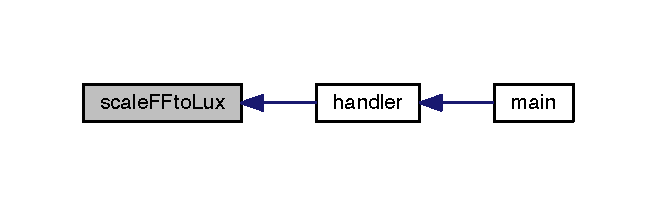
\includegraphics[width=315pt]{db/d85/_lumen_sensor_8c_a4e19311d2241c61d7b3a7ca9cd5fb765_icgraph}
\end{center}
\end{figure}


\index{Lumen\+Sensor.\+c@{Lumen\+Sensor.\+c}!scale\+Lux\+To\+FF@{scale\+Lux\+To\+FF}}
\index{scale\+Lux\+To\+FF@{scale\+Lux\+To\+FF}!Lumen\+Sensor.\+c@{Lumen\+Sensor.\+c}}
\paragraph[{\texorpdfstring{scale\+Lux\+To\+F\+F(unsigned int val)}{scaleLuxToFF(unsigned int val)}}]{\setlength{\rightskip}{0pt plus 5cm}uint8 scale\+Lux\+To\+FF (
\begin{DoxyParamCaption}
\item[{unsigned int}]{val}
\end{DoxyParamCaption}
)}\hypertarget{_lumen_sensor_8c_a1337221b40e407eeb46861aef99c6b83}{}\label{_lumen_sensor_8c_a1337221b40e407eeb46861aef99c6b83}


Scale a lux value into a 0-\/255 range value Due to the limited range to scale into, lux over 1530 is scaled to 255. The top 1530 vas chosen because 1530/255 = 6. 

\begin{DoxyReturn}{Returnerer}
The lux value scaled down into a single uint8 
\end{DoxyReturn}

\begin{DoxyParams}[1]{Parametre}
\mbox{\tt in}  & {\em val} & The lux value to scale down\\
\hline
\end{DoxyParams}
\begin{DoxyAuthor}{Forfatter}
Simon Nejmann (\href{mailto:19981127@uni.au.dk}{\tt 19981127@uni.\+au.\+dk}) 
\end{DoxyAuthor}


Defineret på linje 93 i filen Lumen\+Sensor.\+c.



Refereret til af handler() og scale\+Led\+P\+W\+M().


\begin{DoxyCode}
94 \{
95 \textcolor{comment}{//    int tmp = (val * 255) / 1530;}
96     \textcolor{keywordtype}{int} tmp = val / 6;
97     \textcolor{keywordflow}{return} (uint8)((tmp < 255) ? tmp : 255);
98 \}
\end{DoxyCode}


Her er kalder-\/grafen for denne funktion\+:\nopagebreak
\begin{figure}[H]
\begin{center}
\leavevmode
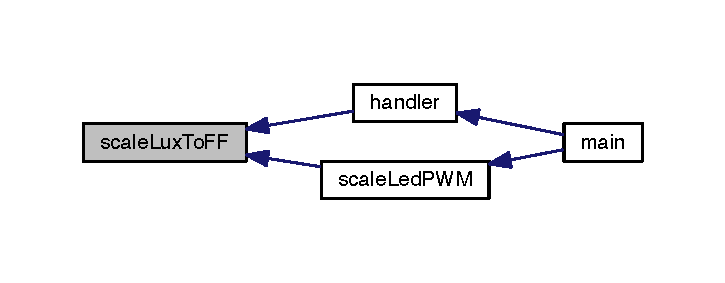
\includegraphics[width=348pt]{db/d85/_lumen_sensor_8c_a1337221b40e407eeb46861aef99c6b83_icgraph}
\end{center}
\end{figure}



\hypertarget{_lumen_sensor_8h}{}\subsection{Lumen\+Sensor.\+h filreference}
\label{_lumen_sensor_8h}\index{Lumen\+Sensor.\+h@{Lumen\+Sensor.\+h}}
{\ttfamily \#include $<$project.\+h$>$}\\*
Inklusions-\/afhængighedsgraf for Lumen\+Sensor.\+h\+:
\nopagebreak
\begin{figure}[H]
\begin{center}
\leavevmode
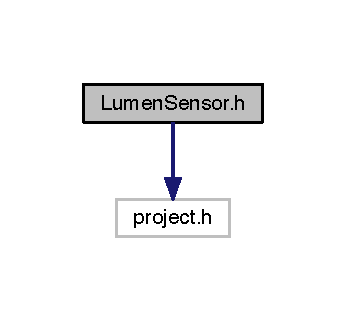
\includegraphics[width=166pt]{d1/d3f/_lumen_sensor_8h__incl}
\end{center}
\end{figure}
Denne graf viser, hvilke filer der direkte eller indirekte inkluderer denne fil\+:
\nopagebreak
\begin{figure}[H]
\begin{center}
\leavevmode
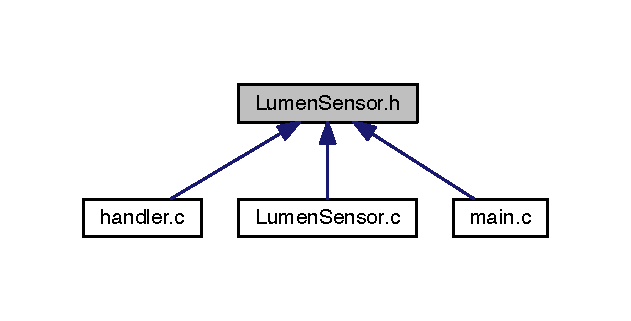
\includegraphics[width=303pt]{d8/d86/_lumen_sensor_8h__dep__incl}
\end{center}
\end{figure}
\subsubsection*{Funktioner}
\begin{DoxyCompactItemize}
\item 
void \hyperlink{_lumen_sensor_8h_a89993394d4ef10fb5362c18ab189ad31}{init\+Lumen\+Sensor} ()
\begin{DoxyCompactList}\small\item\em Initialize the light sensor. \end{DoxyCompactList}\item 
unsigned int \hyperlink{_lumen_sensor_8h_acbfb15efe3f5e10e4de610ba5e3ef9e7}{read\+Lumen\+Sensor} ()
\begin{DoxyCompactList}\small\item\em Read sensor data from the light sensor. \end{DoxyCompactList}\item 
uint8 \hyperlink{_lumen_sensor_8h_a1337221b40e407eeb46861aef99c6b83}{scale\+Lux\+To\+FF} (unsigned int val)
\begin{DoxyCompactList}\small\item\em Scale a lux value into a 0-\/255 range value Due to the limited range to scale into, lux over 1530 is scaled to 255. The top 1530 vas chosen because 1530/255 = 6. \end{DoxyCompactList}\item 
unsigned int \hyperlink{_lumen_sensor_8h_a4e19311d2241c61d7b3a7ca9cd5fb765}{scale\+F\+Fto\+Lux} (uint8 val)
\begin{DoxyCompactList}\small\item\em Scale a 0-\/255 range value into lux Due to the limited input range 1530 has been chosen as max value for lux. The top 1530 vas chosen because 1530/255 = 6. \end{DoxyCompactList}\end{DoxyCompactItemize}


\subsubsection{Funktions-\/dokumentation}
\index{Lumen\+Sensor.\+h@{Lumen\+Sensor.\+h}!init\+Lumen\+Sensor@{init\+Lumen\+Sensor}}
\index{init\+Lumen\+Sensor@{init\+Lumen\+Sensor}!Lumen\+Sensor.\+h@{Lumen\+Sensor.\+h}}
\paragraph[{\texorpdfstring{init\+Lumen\+Sensor()}{initLumenSensor()}}]{\setlength{\rightskip}{0pt plus 5cm}void init\+Lumen\+Sensor (
\begin{DoxyParamCaption}
{}
\end{DoxyParamCaption}
)}\hypertarget{_lumen_sensor_8h_a89993394d4ef10fb5362c18ab189ad31}{}\label{_lumen_sensor_8h_a89993394d4ef10fb5362c18ab189ad31}


Initialize the light sensor. 

\begin{DoxyAuthor}{Forfatter}
Simon Nejmann (\href{mailto:19981127@uni.au.dk}{\tt 19981127@uni.\+au.\+dk}) 
\end{DoxyAuthor}


Defineret på linje 18 i filen Lumen\+Sensor.\+c.



Indeholder referencer til L\+U\+M\+E\+N\+\_\+\+A\+D\+DR.



Refereret til af main().


\begin{DoxyCode}
19 \{
20     uint8 writeBuf[2];
21     uint32 err;
22     
23     \textcolor{comment}{// Add internal pull-up resistors on the SCL and SDA lines}
24     LumenCom\_scl\_SetDriveMode(LumenCom\_scl\_DM\_RES\_UP);
25     LumenCom\_sda\_SetDriveMode(LumenCom\_sda\_DM\_RES\_UP);
26 
27     LumenCom\_Start();
28     \textcolor{comment}{// Send command to sensor:}
29     writeBuf[0] = 0x80; \textcolor{comment}{// Highest bit set = command, low bits 0000 = control register}
30     writeBuf[1] = 0x03; \textcolor{comment}{// Power up sensor}
31     err = LumenCom\_I2CMasterWriteBuf(\hyperlink{_lumen_sensor_8c_aee9d6665305479ca38bc745e6f09a336}{LUMEN\_ADDR}, writeBuf, 2, LumenCom\_I2C\_MODE\_COMPLETE\_XFER);
32     \textcolor{comment}{// Wait for the I2C command to finish transferring:}
33     \textcolor{keywordflow}{while}(LumenCom\_I2CMasterStatus() & LumenCom\_I2C\_MSTAT\_XFER\_INP) \{\}
34 \}
\end{DoxyCode}


Her er kalder-\/grafen for denne funktion\+:
\nopagebreak
\begin{figure}[H]
\begin{center}
\leavevmode
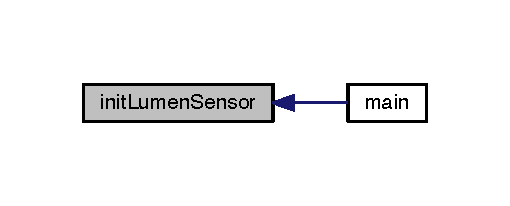
\includegraphics[width=245pt]{df/dac/_lumen_sensor_8h_a89993394d4ef10fb5362c18ab189ad31_icgraph}
\end{center}
\end{figure}


\index{Lumen\+Sensor.\+h@{Lumen\+Sensor.\+h}!read\+Lumen\+Sensor@{read\+Lumen\+Sensor}}
\index{read\+Lumen\+Sensor@{read\+Lumen\+Sensor}!Lumen\+Sensor.\+h@{Lumen\+Sensor.\+h}}
\paragraph[{\texorpdfstring{read\+Lumen\+Sensor()}{readLumenSensor()}}]{\setlength{\rightskip}{0pt plus 5cm}unsigned int read\+Lumen\+Sensor (
\begin{DoxyParamCaption}
{}
\end{DoxyParamCaption}
)}\hypertarget{_lumen_sensor_8h_acbfb15efe3f5e10e4de610ba5e3ef9e7}{}\label{_lumen_sensor_8h_acbfb15efe3f5e10e4de610ba5e3ef9e7}


Read sensor data from the light sensor. 

\begin{DoxyReturn}{Returnerer}
The lux value of the perceived light
\end{DoxyReturn}
\begin{DoxyAuthor}{Forfatter}
Simon Nejmann (\href{mailto:19981127@uni.au.dk}{\tt 19981127@uni.\+au.\+dk}) 
\end{DoxyAuthor}


Defineret på linje 42 i filen Lumen\+Sensor.\+c.



Indeholder referencer til Calculate\+Lux() og L\+U\+M\+E\+N\+\_\+\+A\+D\+DR.



Refereret til af main().


\begin{DoxyCode}
43 \{
44     uint8 readBuf[2];
45     uint8 writeBuf[1];
46     \textcolor{keywordtype}{unsigned} \textcolor{keywordtype}{int} channel0 = 0;
47     \textcolor{keywordtype}{unsigned} \textcolor{keywordtype}{int} channel1 = 0;
48 
49     \textcolor{comment}{// Send "read channel 0" command}
50     writeBuf[0] = 0xAC;
51     LumenCom\_I2CMasterWriteBuf(\hyperlink{_lumen_sensor_8c_aee9d6665305479ca38bc745e6f09a336}{LUMEN\_ADDR}, writeBuf, 1, LumenCom\_I2C\_MODE\_NO\_STOP);
52 
53     \textcolor{comment}{// Wait for the I2C command to finish transferring}
54     \textcolor{keywordflow}{while}(!(LumenCom\_I2CMasterStatus() & LumenCom\_I2C\_MSTAT\_XFER\_HALT)) \{\}
55     \textcolor{comment}{// Read two bytes of data}
56     LumenCom\_I2CMasterReadBuf(\hyperlink{_lumen_sensor_8c_aee9d6665305479ca38bc745e6f09a336}{LUMEN\_ADDR}, readBuf, 2,
57         LumenCom\_I2C\_MODE\_REPEAT\_START | LumenCom\_I2C\_MODE\_NO\_STOP);
58 
59     \textcolor{comment}{// Wait for the I2C command to finish transferring}
60     \textcolor{keywordflow}{while}(!(LumenCom\_I2CMasterStatus() & LumenCom\_I2C\_MSTAT\_XFER\_HALT)) \{\}
61 
62     channel0 = readBuf[0] + readBuf[1] * 256;
63 
64     \textcolor{comment}{// Send "read channel 1" command}
65     writeBuf[0] = 0xAE;
66     LumenCom\_I2CMasterWriteBuf(\hyperlink{_lumen_sensor_8c_aee9d6665305479ca38bc745e6f09a336}{LUMEN\_ADDR}, writeBuf, 1,
67         LumenCom\_I2C\_MODE\_REPEAT\_START | LumenCom\_I2C\_MODE\_NO\_STOP);
68 
69     \textcolor{comment}{// Wait for the I2C command to finish transferring}
70     \textcolor{keywordflow}{while}(!(LumenCom\_I2CMasterStatus() & LumenCom\_I2C\_MSTAT\_XFER\_HALT)) \{\}
71     \textcolor{comment}{// Read two bytes of data}
72     LumenCom\_I2CMasterReadBuf(\hyperlink{_lumen_sensor_8c_aee9d6665305479ca38bc745e6f09a336}{LUMEN\_ADDR}, readBuf, 2, LumenCom\_I2C\_MODE\_REPEAT\_START);
73 
74     \textcolor{comment}{// Wait for the I2C command to finish transferring}
75     \textcolor{keywordflow}{while}(LumenCom\_I2CMasterStatus() & LumenCom\_I2C\_MSTAT\_XFER\_INP) \{\}
76 
77     channel1 = readBuf[0] + readBuf[1] * 256;
78 
79     \textcolor{comment}{// Use Datasheet function to calculate lux value from read values}
80     \textcolor{keywordflow}{return} \hyperlink{lux_8c_a3db2aa0d603f0627be256dc108d3d763}{CalculateLux}(0, 2, channel0, channel1, 0);
81 \}
\end{DoxyCode}


Her er kald-\/grafen for denne funktion\+:
\nopagebreak
\begin{figure}[H]
\begin{center}
\leavevmode
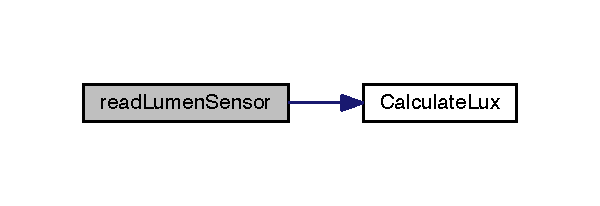
\includegraphics[width=288pt]{df/dac/_lumen_sensor_8h_acbfb15efe3f5e10e4de610ba5e3ef9e7_cgraph}
\end{center}
\end{figure}




Her er kalder-\/grafen for denne funktion\+:
\nopagebreak
\begin{figure}[H]
\begin{center}
\leavevmode
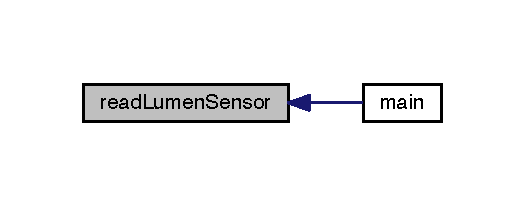
\includegraphics[width=252pt]{df/dac/_lumen_sensor_8h_acbfb15efe3f5e10e4de610ba5e3ef9e7_icgraph}
\end{center}
\end{figure}


\index{Lumen\+Sensor.\+h@{Lumen\+Sensor.\+h}!scale\+F\+Fto\+Lux@{scale\+F\+Fto\+Lux}}
\index{scale\+F\+Fto\+Lux@{scale\+F\+Fto\+Lux}!Lumen\+Sensor.\+h@{Lumen\+Sensor.\+h}}
\paragraph[{\texorpdfstring{scale\+F\+Fto\+Lux(uint8 val)}{scaleFFtoLux(uint8 val)}}]{\setlength{\rightskip}{0pt plus 5cm}unsigned int scale\+F\+Fto\+Lux (
\begin{DoxyParamCaption}
\item[{uint8}]{val}
\end{DoxyParamCaption}
)}\hypertarget{_lumen_sensor_8h_a4e19311d2241c61d7b3a7ca9cd5fb765}{}\label{_lumen_sensor_8h_a4e19311d2241c61d7b3a7ca9cd5fb765}


Scale a 0-\/255 range value into lux Due to the limited input range 1530 has been chosen as max value for lux. The top 1530 vas chosen because 1530/255 = 6. 

\begin{DoxyReturn}{Returnerer}
The an upscaled lux value 
\end{DoxyReturn}

\begin{DoxyParams}[1]{Parametre}
\mbox{\tt in}  & {\em val} & uint8 containing a value to scale up\\
\hline
\end{DoxyParams}
\begin{DoxyAuthor}{Forfatter}
Simon Nejmann (\href{mailto:19981127@uni.au.dk}{\tt 19981127@uni.\+au.\+dk}) 
\end{DoxyAuthor}


Defineret på linje 110 i filen Lumen\+Sensor.\+c.



Refereret til af handler().


\begin{DoxyCode}
111 \{
112 \textcolor{comment}{//    return  (val * 1530) / 255;}
113     \textcolor{keywordflow}{return}  val * 6;
114 \}
\end{DoxyCode}


Her er kalder-\/grafen for denne funktion\+:
\nopagebreak
\begin{figure}[H]
\begin{center}
\leavevmode
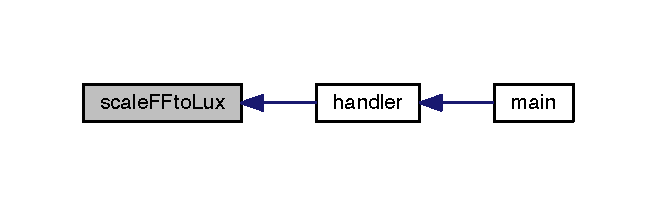
\includegraphics[width=315pt]{df/dac/_lumen_sensor_8h_a4e19311d2241c61d7b3a7ca9cd5fb765_icgraph}
\end{center}
\end{figure}


\index{Lumen\+Sensor.\+h@{Lumen\+Sensor.\+h}!scale\+Lux\+To\+FF@{scale\+Lux\+To\+FF}}
\index{scale\+Lux\+To\+FF@{scale\+Lux\+To\+FF}!Lumen\+Sensor.\+h@{Lumen\+Sensor.\+h}}
\paragraph[{\texorpdfstring{scale\+Lux\+To\+F\+F(unsigned int val)}{scaleLuxToFF(unsigned int val)}}]{\setlength{\rightskip}{0pt plus 5cm}uint8 scale\+Lux\+To\+FF (
\begin{DoxyParamCaption}
\item[{unsigned int}]{val}
\end{DoxyParamCaption}
)}\hypertarget{_lumen_sensor_8h_a1337221b40e407eeb46861aef99c6b83}{}\label{_lumen_sensor_8h_a1337221b40e407eeb46861aef99c6b83}


Scale a lux value into a 0-\/255 range value Due to the limited range to scale into, lux over 1530 is scaled to 255. The top 1530 vas chosen because 1530/255 = 6. 

\begin{DoxyReturn}{Returnerer}
The lux value scaled down into a single uint8 
\end{DoxyReturn}

\begin{DoxyParams}[1]{Parametre}
\mbox{\tt in}  & {\em val} & The lux value to scale down\\
\hline
\end{DoxyParams}
\begin{DoxyAuthor}{Forfatter}
Simon Nejmann (\href{mailto:19981127@uni.au.dk}{\tt 19981127@uni.\+au.\+dk}) 
\end{DoxyAuthor}


Defineret på linje 93 i filen Lumen\+Sensor.\+c.



Refereret til af handler() og scale\+Led\+P\+W\+M().


\begin{DoxyCode}
94 \{
95 \textcolor{comment}{//    int tmp = (val * 255) / 1530;}
96     \textcolor{keywordtype}{int} tmp = val / 6;
97     \textcolor{keywordflow}{return} (uint8)((tmp < 255) ? tmp : 255);
98 \}
\end{DoxyCode}


Her er kalder-\/grafen for denne funktion\+:
\nopagebreak
\begin{figure}[H]
\begin{center}
\leavevmode
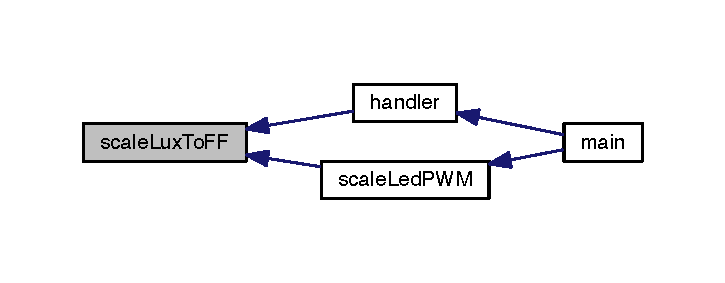
\includegraphics[width=348pt]{df/dac/_lumen_sensor_8h_a1337221b40e407eeb46861aef99c6b83_icgraph}
\end{center}
\end{figure}



\hypertarget{lux_8c}{}\subsection{lux.\+c filreference}
\label{lux_8c}\index{lux.\+c@{lux.\+c}}


Code copied from the \char`\"{}\+T\+S\+L2561 Light-\/to-\/digital converter\char`\"{} datasheet.  


\subsubsection*{\#Defines}
\begin{DoxyCompactItemize}
\item 
\#define \hyperlink{lux_8c_abe3540b1f05e5974dfa40491719b322a}{L\+U\+X\+\_\+\+S\+C\+A\+LE}~14
\item 
\#define \hyperlink{lux_8c_a2d36ccf8157f890c015eddd64276d77c}{R\+A\+T\+I\+O\+\_\+\+S\+C\+A\+LE}~9
\item 
\#define \hyperlink{lux_8c_ae77b11d54490369c690da18aef1e76e5}{C\+H\+\_\+\+S\+C\+A\+LE}~10
\item 
\#define \hyperlink{lux_8c_af740a064eaa0da3339e7eba683a671ed}{C\+H\+S\+C\+A\+L\+E\+\_\+\+T\+I\+N\+T0}~0x7517
\item 
\#define \hyperlink{lux_8c_a1f741d16494e81486136c73489097cdd}{C\+H\+S\+C\+A\+L\+E\+\_\+\+T\+I\+N\+T1}~0x0fe7
\item 
\#define \hyperlink{lux_8c_a8d1758888413b06317d05260d023c6f1}{K1T}~0x0040
\item 
\#define \hyperlink{lux_8c_a77a115660299dfe589547bd1c9313e18}{B1T}~0x01f2
\item 
\#define \hyperlink{lux_8c_a9cee464de95fd9f1cc41e4737cdfcf56}{M1T}~0x01be
\item 
\#define \hyperlink{lux_8c_af3f76dac869af6d4fb8834ba8e5baa72}{K2T}~0x0080
\item 
\#define \hyperlink{lux_8c_a0a24c8d38c744a6706fbef06cc0d045e}{B2T}~0x0214
\item 
\#define \hyperlink{lux_8c_af13d82736a980dd7f78a0c8633c656c0}{M2T}~0x02d1
\item 
\#define \hyperlink{lux_8c_a96898795c866703216e3035ecc1c29aa}{K3T}~0x00c0
\item 
\#define \hyperlink{lux_8c_aa58a8a3b4010f1d8ab947e2351b6cf1d}{B3T}~0x023f
\item 
\#define \hyperlink{lux_8c_a6d02cd58020bf44d98927446668a2f7b}{M3T}~0x037b
\item 
\#define \hyperlink{lux_8c_aa3489bee2d8a1e25002669517f4b6f7d}{K4T}~0x0100
\item 
\#define \hyperlink{lux_8c_a836fd96912939cd386f83e20ed1061ee}{B4T}~0x0270
\item 
\#define \hyperlink{lux_8c_ac5983b281c3a2f1d4ea1f87236cfcb44}{M4T}~0x03fe
\item 
\#define \hyperlink{lux_8c_a7df915d6ba425afa9a463f249168d6bd}{K5T}~0x0138
\item 
\#define \hyperlink{lux_8c_a8a3732432706e9a5a5ae3d3485d47043}{B5T}~0x016f
\item 
\#define \hyperlink{lux_8c_a2d9fce4a16f258b5ab02b09a954648f6}{M5T}~0x01fc
\item 
\#define \hyperlink{lux_8c_a677e2edf3cf15bef63405c35a7be1310}{K6T}~0x019a
\item 
\#define \hyperlink{lux_8c_ab01465ad82a39e8d02c2dd79279bfe38}{B6T}~0x00d2
\item 
\#define \hyperlink{lux_8c_a48074a633649636c0748b851a23776df}{M6T}~0x00fb
\item 
\#define \hyperlink{lux_8c_a7e788fd48d058b89ffcc0438bc3d558e}{K7T}~0x029a
\item 
\#define \hyperlink{lux_8c_ad61180572632999584ac8b582a00e2c8}{B7T}~0x0018
\item 
\#define \hyperlink{lux_8c_aa3094566ff7a1a2bcd210e256c7b50cc}{M7T}~0x0012
\item 
\#define \hyperlink{lux_8c_aa0dc3961e2039ad7d91faf6829ec1404}{K8T}~0x029a
\item 
\#define \hyperlink{lux_8c_ab5d069e613c69aaf71ea97b129cc5ec1}{B8T}~0x0000
\item 
\#define \hyperlink{lux_8c_acb54eadab753bfe327548d7216edd9a2}{M8T}~0x0000
\item 
\#define \hyperlink{lux_8c_a5d91e3222633d82540d7ce0e8d2e1bb2}{K1C}~0x0043
\item 
\#define \hyperlink{lux_8c_a93aa8f0bb51f43d51e78656a352c6d16}{B1C}~0x0204
\item 
\#define \hyperlink{lux_8c_a4ec6175326ca3eb8b731a162b6fcd866}{M1C}~0x01ad
\item 
\#define \hyperlink{lux_8c_ac91e954471045fdbd9b3d01933373c1e}{K2C}~0x0085
\item 
\#define \hyperlink{lux_8c_a95f02da704fdc6c1cabd0c29713cee66}{B2C}~0x0228
\item 
\#define \hyperlink{lux_8c_ab70590fa6ebed50a3ab8ff17c22b55b2}{M2C}~0x02c1
\item 
\#define \hyperlink{lux_8c_acbc83f137380f27faf46af997f35f882}{K3C}~0x00c8
\item 
\#define \hyperlink{lux_8c_ac03c4526fc8c17d71c8ee2171537facd}{B3C}~0x0253
\item 
\#define \hyperlink{lux_8c_a172d826f878378caa7889305ad29011f}{M3C}~0x0363
\item 
\#define \hyperlink{lux_8c_a2fccbc87358653185282ba16b03a64ee}{K4C}~0x010a
\item 
\#define \hyperlink{lux_8c_a6bd8165e32f19978994245c552b8ee2d}{B4C}~0x0282
\item 
\#define \hyperlink{lux_8c_abca79308fb0392b1f8c9d5cfeb5310a0}{M4C}~0x03df
\item 
\#define \hyperlink{lux_8c_aa39a8eec5ffe9f84c4ac098724c70c91}{K5C}~0x014d
\item 
\#define \hyperlink{lux_8c_af4a1b651ec51bb418ce1bffb87fa79e4}{B5C}~0x0177
\item 
\#define \hyperlink{lux_8c_a7c5adce134d8d2be44024c075f55c5c1}{M5C}~0x01dd
\item 
\#define \hyperlink{lux_8c_a9dccc63bcf43c1b4714e913053a906c1}{K6C}~0x019a
\item 
\#define \hyperlink{lux_8c_abe71d8a87f6d974ee3d26693d1a2ea51}{B6C}~0x0101
\item 
\#define \hyperlink{lux_8c_a2140b89133d826e76d2a717a3d863551}{M6C}~0x0127
\item 
\#define \hyperlink{lux_8c_ac104bf3b33df4e42b14dc31078283565}{K7C}~0x029a
\item 
\#define \hyperlink{lux_8c_a5750be8469107d68ea4bdd4e4947316b}{B7C}~0x0037
\item 
\#define \hyperlink{lux_8c_acc5b1974656133787900e9bd5219c5ce}{M7C}~0x002b
\item 
\#define \hyperlink{lux_8c_ac47a903b8bc65dc56915024f00201213}{K8C}~0x029a
\item 
\#define \hyperlink{lux_8c_a6d9dfce0cef08b9ef488e582ac4f92e9}{B8C}~0x0000
\item 
\#define \hyperlink{lux_8c_ac15c8f99823ed2ff447fb568ce4d3957}{M8C}~0x0000
\end{DoxyCompactItemize}
\subsubsection*{Funktioner}
\begin{DoxyCompactItemize}
\item 
unsigned int \hyperlink{lux_8c_a3db2aa0d603f0627be256dc108d3d763}{Calculate\+Lux} (unsigned int i\+Gain, unsigned int t\+Int, unsigned int ch0, unsigned int ch1, int i\+Type)
\begin{DoxyCompactList}\small\item\em Calculate perceived lux from sensor values The sensor has two detectors, one that detects visible and infrared light while the second only detects infrared light. The amount of visible light is then calculated by substracting a scaling fraction of the second detector value from a scaling fraction of the first. \end{DoxyCompactList}\end{DoxyCompactItemize}


\subsubsection{Detaljeret beskrivelse}
Code copied from the \char`\"{}\+T\+S\+L2561 Light-\/to-\/digital converter\char`\"{} datasheet. 

\begin{DoxyAuthor}{Forfatter}
T\+A\+OS, Inc. 
\end{DoxyAuthor}


\subsubsection{\#Define-\/dokumentation}
\index{lux.\+c@{lux.\+c}!B1C@{B1C}}
\index{B1C@{B1C}!lux.\+c@{lux.\+c}}
\paragraph[{\texorpdfstring{B1C}{B1C}}]{\setlength{\rightskip}{0pt plus 5cm}\#define B1C~0x0204}\hypertarget{lux_8c_a93aa8f0bb51f43d51e78656a352c6d16}{}\label{lux_8c_a93aa8f0bb51f43d51e78656a352c6d16}


Defineret på linje 106 i filen lux.\+c.



Refereret til af Calculate\+Lux().

\index{lux.\+c@{lux.\+c}!B1T@{B1T}}
\index{B1T@{B1T}!lux.\+c@{lux.\+c}}
\paragraph[{\texorpdfstring{B1T}{B1T}}]{\setlength{\rightskip}{0pt plus 5cm}\#define B1T~0x01f2}\hypertarget{lux_8c_a77a115660299dfe589547bd1c9313e18}{}\label{lux_8c_a77a115660299dfe589547bd1c9313e18}


Defineret på linje 59 i filen lux.\+c.



Refereret til af Calculate\+Lux().

\index{lux.\+c@{lux.\+c}!B2C@{B2C}}
\index{B2C@{B2C}!lux.\+c@{lux.\+c}}
\paragraph[{\texorpdfstring{B2C}{B2C}}]{\setlength{\rightskip}{0pt plus 5cm}\#define B2C~0x0228}\hypertarget{lux_8c_a95f02da704fdc6c1cabd0c29713cee66}{}\label{lux_8c_a95f02da704fdc6c1cabd0c29713cee66}


Defineret på linje 109 i filen lux.\+c.



Refereret til af Calculate\+Lux().

\index{lux.\+c@{lux.\+c}!B2T@{B2T}}
\index{B2T@{B2T}!lux.\+c@{lux.\+c}}
\paragraph[{\texorpdfstring{B2T}{B2T}}]{\setlength{\rightskip}{0pt plus 5cm}\#define B2T~0x0214}\hypertarget{lux_8c_a0a24c8d38c744a6706fbef06cc0d045e}{}\label{lux_8c_a0a24c8d38c744a6706fbef06cc0d045e}


Defineret på linje 62 i filen lux.\+c.



Refereret til af Calculate\+Lux().

\index{lux.\+c@{lux.\+c}!B3C@{B3C}}
\index{B3C@{B3C}!lux.\+c@{lux.\+c}}
\paragraph[{\texorpdfstring{B3C}{B3C}}]{\setlength{\rightskip}{0pt plus 5cm}\#define B3C~0x0253}\hypertarget{lux_8c_ac03c4526fc8c17d71c8ee2171537facd}{}\label{lux_8c_ac03c4526fc8c17d71c8ee2171537facd}


Defineret på linje 112 i filen lux.\+c.



Refereret til af Calculate\+Lux().

\index{lux.\+c@{lux.\+c}!B3T@{B3T}}
\index{B3T@{B3T}!lux.\+c@{lux.\+c}}
\paragraph[{\texorpdfstring{B3T}{B3T}}]{\setlength{\rightskip}{0pt plus 5cm}\#define B3T~0x023f}\hypertarget{lux_8c_aa58a8a3b4010f1d8ab947e2351b6cf1d}{}\label{lux_8c_aa58a8a3b4010f1d8ab947e2351b6cf1d}


Defineret på linje 65 i filen lux.\+c.



Refereret til af Calculate\+Lux().

\index{lux.\+c@{lux.\+c}!B4C@{B4C}}
\index{B4C@{B4C}!lux.\+c@{lux.\+c}}
\paragraph[{\texorpdfstring{B4C}{B4C}}]{\setlength{\rightskip}{0pt plus 5cm}\#define B4C~0x0282}\hypertarget{lux_8c_a6bd8165e32f19978994245c552b8ee2d}{}\label{lux_8c_a6bd8165e32f19978994245c552b8ee2d}


Defineret på linje 115 i filen lux.\+c.



Refereret til af Calculate\+Lux().

\index{lux.\+c@{lux.\+c}!B4T@{B4T}}
\index{B4T@{B4T}!lux.\+c@{lux.\+c}}
\paragraph[{\texorpdfstring{B4T}{B4T}}]{\setlength{\rightskip}{0pt plus 5cm}\#define B4T~0x0270}\hypertarget{lux_8c_a836fd96912939cd386f83e20ed1061ee}{}\label{lux_8c_a836fd96912939cd386f83e20ed1061ee}


Defineret på linje 68 i filen lux.\+c.



Refereret til af Calculate\+Lux().

\index{lux.\+c@{lux.\+c}!B5C@{B5C}}
\index{B5C@{B5C}!lux.\+c@{lux.\+c}}
\paragraph[{\texorpdfstring{B5C}{B5C}}]{\setlength{\rightskip}{0pt plus 5cm}\#define B5C~0x0177}\hypertarget{lux_8c_af4a1b651ec51bb418ce1bffb87fa79e4}{}\label{lux_8c_af4a1b651ec51bb418ce1bffb87fa79e4}


Defineret på linje 118 i filen lux.\+c.



Refereret til af Calculate\+Lux().

\index{lux.\+c@{lux.\+c}!B5T@{B5T}}
\index{B5T@{B5T}!lux.\+c@{lux.\+c}}
\paragraph[{\texorpdfstring{B5T}{B5T}}]{\setlength{\rightskip}{0pt plus 5cm}\#define B5T~0x016f}\hypertarget{lux_8c_a8a3732432706e9a5a5ae3d3485d47043}{}\label{lux_8c_a8a3732432706e9a5a5ae3d3485d47043}


Defineret på linje 71 i filen lux.\+c.



Refereret til af Calculate\+Lux().

\index{lux.\+c@{lux.\+c}!B6C@{B6C}}
\index{B6C@{B6C}!lux.\+c@{lux.\+c}}
\paragraph[{\texorpdfstring{B6C}{B6C}}]{\setlength{\rightskip}{0pt plus 5cm}\#define B6C~0x0101}\hypertarget{lux_8c_abe71d8a87f6d974ee3d26693d1a2ea51}{}\label{lux_8c_abe71d8a87f6d974ee3d26693d1a2ea51}


Defineret på linje 121 i filen lux.\+c.



Refereret til af Calculate\+Lux().

\index{lux.\+c@{lux.\+c}!B6T@{B6T}}
\index{B6T@{B6T}!lux.\+c@{lux.\+c}}
\paragraph[{\texorpdfstring{B6T}{B6T}}]{\setlength{\rightskip}{0pt plus 5cm}\#define B6T~0x00d2}\hypertarget{lux_8c_ab01465ad82a39e8d02c2dd79279bfe38}{}\label{lux_8c_ab01465ad82a39e8d02c2dd79279bfe38}


Defineret på linje 74 i filen lux.\+c.



Refereret til af Calculate\+Lux().

\index{lux.\+c@{lux.\+c}!B7C@{B7C}}
\index{B7C@{B7C}!lux.\+c@{lux.\+c}}
\paragraph[{\texorpdfstring{B7C}{B7C}}]{\setlength{\rightskip}{0pt plus 5cm}\#define B7C~0x0037}\hypertarget{lux_8c_a5750be8469107d68ea4bdd4e4947316b}{}\label{lux_8c_a5750be8469107d68ea4bdd4e4947316b}


Defineret på linje 124 i filen lux.\+c.



Refereret til af Calculate\+Lux().

\index{lux.\+c@{lux.\+c}!B7T@{B7T}}
\index{B7T@{B7T}!lux.\+c@{lux.\+c}}
\paragraph[{\texorpdfstring{B7T}{B7T}}]{\setlength{\rightskip}{0pt plus 5cm}\#define B7T~0x0018}\hypertarget{lux_8c_ad61180572632999584ac8b582a00e2c8}{}\label{lux_8c_ad61180572632999584ac8b582a00e2c8}


Defineret på linje 77 i filen lux.\+c.



Refereret til af Calculate\+Lux().

\index{lux.\+c@{lux.\+c}!B8C@{B8C}}
\index{B8C@{B8C}!lux.\+c@{lux.\+c}}
\paragraph[{\texorpdfstring{B8C}{B8C}}]{\setlength{\rightskip}{0pt plus 5cm}\#define B8C~0x0000}\hypertarget{lux_8c_a6d9dfce0cef08b9ef488e582ac4f92e9}{}\label{lux_8c_a6d9dfce0cef08b9ef488e582ac4f92e9}


Defineret på linje 127 i filen lux.\+c.



Refereret til af Calculate\+Lux().

\index{lux.\+c@{lux.\+c}!B8T@{B8T}}
\index{B8T@{B8T}!lux.\+c@{lux.\+c}}
\paragraph[{\texorpdfstring{B8T}{B8T}}]{\setlength{\rightskip}{0pt plus 5cm}\#define B8T~0x0000}\hypertarget{lux_8c_ab5d069e613c69aaf71ea97b129cc5ec1}{}\label{lux_8c_ab5d069e613c69aaf71ea97b129cc5ec1}


Defineret på linje 80 i filen lux.\+c.



Refereret til af Calculate\+Lux().

\index{lux.\+c@{lux.\+c}!C\+H\+\_\+\+S\+C\+A\+LE@{C\+H\+\_\+\+S\+C\+A\+LE}}
\index{C\+H\+\_\+\+S\+C\+A\+LE@{C\+H\+\_\+\+S\+C\+A\+LE}!lux.\+c@{lux.\+c}}
\paragraph[{\texorpdfstring{C\+H\+\_\+\+S\+C\+A\+LE}{CH_SCALE}}]{\setlength{\rightskip}{0pt plus 5cm}\#define C\+H\+\_\+\+S\+C\+A\+LE~10}\hypertarget{lux_8c_ae77b11d54490369c690da18aef1e76e5}{}\label{lux_8c_ae77b11d54490369c690da18aef1e76e5}


Defineret på linje 25 i filen lux.\+c.



Refereret til af Calculate\+Lux().

\index{lux.\+c@{lux.\+c}!C\+H\+S\+C\+A\+L\+E\+\_\+\+T\+I\+N\+T0@{C\+H\+S\+C\+A\+L\+E\+\_\+\+T\+I\+N\+T0}}
\index{C\+H\+S\+C\+A\+L\+E\+\_\+\+T\+I\+N\+T0@{C\+H\+S\+C\+A\+L\+E\+\_\+\+T\+I\+N\+T0}!lux.\+c@{lux.\+c}}
\paragraph[{\texorpdfstring{C\+H\+S\+C\+A\+L\+E\+\_\+\+T\+I\+N\+T0}{CHSCALE_TINT0}}]{\setlength{\rightskip}{0pt plus 5cm}\#define C\+H\+S\+C\+A\+L\+E\+\_\+\+T\+I\+N\+T0~0x7517}\hypertarget{lux_8c_af740a064eaa0da3339e7eba683a671ed}{}\label{lux_8c_af740a064eaa0da3339e7eba683a671ed}


Defineret på linje 26 i filen lux.\+c.



Refereret til af Calculate\+Lux().

\index{lux.\+c@{lux.\+c}!C\+H\+S\+C\+A\+L\+E\+\_\+\+T\+I\+N\+T1@{C\+H\+S\+C\+A\+L\+E\+\_\+\+T\+I\+N\+T1}}
\index{C\+H\+S\+C\+A\+L\+E\+\_\+\+T\+I\+N\+T1@{C\+H\+S\+C\+A\+L\+E\+\_\+\+T\+I\+N\+T1}!lux.\+c@{lux.\+c}}
\paragraph[{\texorpdfstring{C\+H\+S\+C\+A\+L\+E\+\_\+\+T\+I\+N\+T1}{CHSCALE_TINT1}}]{\setlength{\rightskip}{0pt plus 5cm}\#define C\+H\+S\+C\+A\+L\+E\+\_\+\+T\+I\+N\+T1~0x0fe7}\hypertarget{lux_8c_a1f741d16494e81486136c73489097cdd}{}\label{lux_8c_a1f741d16494e81486136c73489097cdd}


Defineret på linje 27 i filen lux.\+c.



Refereret til af Calculate\+Lux().

\index{lux.\+c@{lux.\+c}!K1C@{K1C}}
\index{K1C@{K1C}!lux.\+c@{lux.\+c}}
\paragraph[{\texorpdfstring{K1C}{K1C}}]{\setlength{\rightskip}{0pt plus 5cm}\#define K1C~0x0043}\hypertarget{lux_8c_a5d91e3222633d82540d7ce0e8d2e1bb2}{}\label{lux_8c_a5d91e3222633d82540d7ce0e8d2e1bb2}


Defineret på linje 105 i filen lux.\+c.



Refereret til af Calculate\+Lux().

\index{lux.\+c@{lux.\+c}!K1T@{K1T}}
\index{K1T@{K1T}!lux.\+c@{lux.\+c}}
\paragraph[{\texorpdfstring{K1T}{K1T}}]{\setlength{\rightskip}{0pt plus 5cm}\#define K1T~0x0040}\hypertarget{lux_8c_a8d1758888413b06317d05260d023c6f1}{}\label{lux_8c_a8d1758888413b06317d05260d023c6f1}


Defineret på linje 58 i filen lux.\+c.



Refereret til af Calculate\+Lux().

\index{lux.\+c@{lux.\+c}!K2C@{K2C}}
\index{K2C@{K2C}!lux.\+c@{lux.\+c}}
\paragraph[{\texorpdfstring{K2C}{K2C}}]{\setlength{\rightskip}{0pt plus 5cm}\#define K2C~0x0085}\hypertarget{lux_8c_ac91e954471045fdbd9b3d01933373c1e}{}\label{lux_8c_ac91e954471045fdbd9b3d01933373c1e}


Defineret på linje 108 i filen lux.\+c.



Refereret til af Calculate\+Lux().

\index{lux.\+c@{lux.\+c}!K2T@{K2T}}
\index{K2T@{K2T}!lux.\+c@{lux.\+c}}
\paragraph[{\texorpdfstring{K2T}{K2T}}]{\setlength{\rightskip}{0pt plus 5cm}\#define K2T~0x0080}\hypertarget{lux_8c_af3f76dac869af6d4fb8834ba8e5baa72}{}\label{lux_8c_af3f76dac869af6d4fb8834ba8e5baa72}


Defineret på linje 61 i filen lux.\+c.



Refereret til af Calculate\+Lux().

\index{lux.\+c@{lux.\+c}!K3C@{K3C}}
\index{K3C@{K3C}!lux.\+c@{lux.\+c}}
\paragraph[{\texorpdfstring{K3C}{K3C}}]{\setlength{\rightskip}{0pt plus 5cm}\#define K3C~0x00c8}\hypertarget{lux_8c_acbc83f137380f27faf46af997f35f882}{}\label{lux_8c_acbc83f137380f27faf46af997f35f882}


Defineret på linje 111 i filen lux.\+c.



Refereret til af Calculate\+Lux().

\index{lux.\+c@{lux.\+c}!K3T@{K3T}}
\index{K3T@{K3T}!lux.\+c@{lux.\+c}}
\paragraph[{\texorpdfstring{K3T}{K3T}}]{\setlength{\rightskip}{0pt plus 5cm}\#define K3T~0x00c0}\hypertarget{lux_8c_a96898795c866703216e3035ecc1c29aa}{}\label{lux_8c_a96898795c866703216e3035ecc1c29aa}


Defineret på linje 64 i filen lux.\+c.



Refereret til af Calculate\+Lux().

\index{lux.\+c@{lux.\+c}!K4C@{K4C}}
\index{K4C@{K4C}!lux.\+c@{lux.\+c}}
\paragraph[{\texorpdfstring{K4C}{K4C}}]{\setlength{\rightskip}{0pt plus 5cm}\#define K4C~0x010a}\hypertarget{lux_8c_a2fccbc87358653185282ba16b03a64ee}{}\label{lux_8c_a2fccbc87358653185282ba16b03a64ee}


Defineret på linje 114 i filen lux.\+c.



Refereret til af Calculate\+Lux().

\index{lux.\+c@{lux.\+c}!K4T@{K4T}}
\index{K4T@{K4T}!lux.\+c@{lux.\+c}}
\paragraph[{\texorpdfstring{K4T}{K4T}}]{\setlength{\rightskip}{0pt plus 5cm}\#define K4T~0x0100}\hypertarget{lux_8c_aa3489bee2d8a1e25002669517f4b6f7d}{}\label{lux_8c_aa3489bee2d8a1e25002669517f4b6f7d}


Defineret på linje 67 i filen lux.\+c.



Refereret til af Calculate\+Lux().

\index{lux.\+c@{lux.\+c}!K5C@{K5C}}
\index{K5C@{K5C}!lux.\+c@{lux.\+c}}
\paragraph[{\texorpdfstring{K5C}{K5C}}]{\setlength{\rightskip}{0pt plus 5cm}\#define K5C~0x014d}\hypertarget{lux_8c_aa39a8eec5ffe9f84c4ac098724c70c91}{}\label{lux_8c_aa39a8eec5ffe9f84c4ac098724c70c91}


Defineret på linje 117 i filen lux.\+c.



Refereret til af Calculate\+Lux().

\index{lux.\+c@{lux.\+c}!K5T@{K5T}}
\index{K5T@{K5T}!lux.\+c@{lux.\+c}}
\paragraph[{\texorpdfstring{K5T}{K5T}}]{\setlength{\rightskip}{0pt plus 5cm}\#define K5T~0x0138}\hypertarget{lux_8c_a7df915d6ba425afa9a463f249168d6bd}{}\label{lux_8c_a7df915d6ba425afa9a463f249168d6bd}


Defineret på linje 70 i filen lux.\+c.



Refereret til af Calculate\+Lux().

\index{lux.\+c@{lux.\+c}!K6C@{K6C}}
\index{K6C@{K6C}!lux.\+c@{lux.\+c}}
\paragraph[{\texorpdfstring{K6C}{K6C}}]{\setlength{\rightskip}{0pt plus 5cm}\#define K6C~0x019a}\hypertarget{lux_8c_a9dccc63bcf43c1b4714e913053a906c1}{}\label{lux_8c_a9dccc63bcf43c1b4714e913053a906c1}


Defineret på linje 120 i filen lux.\+c.



Refereret til af Calculate\+Lux().

\index{lux.\+c@{lux.\+c}!K6T@{K6T}}
\index{K6T@{K6T}!lux.\+c@{lux.\+c}}
\paragraph[{\texorpdfstring{K6T}{K6T}}]{\setlength{\rightskip}{0pt plus 5cm}\#define K6T~0x019a}\hypertarget{lux_8c_a677e2edf3cf15bef63405c35a7be1310}{}\label{lux_8c_a677e2edf3cf15bef63405c35a7be1310}


Defineret på linje 73 i filen lux.\+c.



Refereret til af Calculate\+Lux().

\index{lux.\+c@{lux.\+c}!K7C@{K7C}}
\index{K7C@{K7C}!lux.\+c@{lux.\+c}}
\paragraph[{\texorpdfstring{K7C}{K7C}}]{\setlength{\rightskip}{0pt plus 5cm}\#define K7C~0x029a}\hypertarget{lux_8c_ac104bf3b33df4e42b14dc31078283565}{}\label{lux_8c_ac104bf3b33df4e42b14dc31078283565}


Defineret på linje 123 i filen lux.\+c.



Refereret til af Calculate\+Lux().

\index{lux.\+c@{lux.\+c}!K7T@{K7T}}
\index{K7T@{K7T}!lux.\+c@{lux.\+c}}
\paragraph[{\texorpdfstring{K7T}{K7T}}]{\setlength{\rightskip}{0pt plus 5cm}\#define K7T~0x029a}\hypertarget{lux_8c_a7e788fd48d058b89ffcc0438bc3d558e}{}\label{lux_8c_a7e788fd48d058b89ffcc0438bc3d558e}


Defineret på linje 76 i filen lux.\+c.



Refereret til af Calculate\+Lux().

\index{lux.\+c@{lux.\+c}!K8C@{K8C}}
\index{K8C@{K8C}!lux.\+c@{lux.\+c}}
\paragraph[{\texorpdfstring{K8C}{K8C}}]{\setlength{\rightskip}{0pt plus 5cm}\#define K8C~0x029a}\hypertarget{lux_8c_ac47a903b8bc65dc56915024f00201213}{}\label{lux_8c_ac47a903b8bc65dc56915024f00201213}


Defineret på linje 126 i filen lux.\+c.



Refereret til af Calculate\+Lux().

\index{lux.\+c@{lux.\+c}!K8T@{K8T}}
\index{K8T@{K8T}!lux.\+c@{lux.\+c}}
\paragraph[{\texorpdfstring{K8T}{K8T}}]{\setlength{\rightskip}{0pt plus 5cm}\#define K8T~0x029a}\hypertarget{lux_8c_aa0dc3961e2039ad7d91faf6829ec1404}{}\label{lux_8c_aa0dc3961e2039ad7d91faf6829ec1404}


Defineret på linje 79 i filen lux.\+c.



Refereret til af Calculate\+Lux().

\index{lux.\+c@{lux.\+c}!L\+U\+X\+\_\+\+S\+C\+A\+LE@{L\+U\+X\+\_\+\+S\+C\+A\+LE}}
\index{L\+U\+X\+\_\+\+S\+C\+A\+LE@{L\+U\+X\+\_\+\+S\+C\+A\+LE}!lux.\+c@{lux.\+c}}
\paragraph[{\texorpdfstring{L\+U\+X\+\_\+\+S\+C\+A\+LE}{LUX_SCALE}}]{\setlength{\rightskip}{0pt plus 5cm}\#define L\+U\+X\+\_\+\+S\+C\+A\+LE~14}\hypertarget{lux_8c_abe3540b1f05e5974dfa40491719b322a}{}\label{lux_8c_abe3540b1f05e5974dfa40491719b322a}


Defineret på linje 20 i filen lux.\+c.



Refereret til af Calculate\+Lux().

\index{lux.\+c@{lux.\+c}!M1C@{M1C}}
\index{M1C@{M1C}!lux.\+c@{lux.\+c}}
\paragraph[{\texorpdfstring{M1C}{M1C}}]{\setlength{\rightskip}{0pt plus 5cm}\#define M1C~0x01ad}\hypertarget{lux_8c_a4ec6175326ca3eb8b731a162b6fcd866}{}\label{lux_8c_a4ec6175326ca3eb8b731a162b6fcd866}


Defineret på linje 107 i filen lux.\+c.



Refereret til af Calculate\+Lux().

\index{lux.\+c@{lux.\+c}!M1T@{M1T}}
\index{M1T@{M1T}!lux.\+c@{lux.\+c}}
\paragraph[{\texorpdfstring{M1T}{M1T}}]{\setlength{\rightskip}{0pt plus 5cm}\#define M1T~0x01be}\hypertarget{lux_8c_a9cee464de95fd9f1cc41e4737cdfcf56}{}\label{lux_8c_a9cee464de95fd9f1cc41e4737cdfcf56}


Defineret på linje 60 i filen lux.\+c.



Refereret til af Calculate\+Lux().

\index{lux.\+c@{lux.\+c}!M2C@{M2C}}
\index{M2C@{M2C}!lux.\+c@{lux.\+c}}
\paragraph[{\texorpdfstring{M2C}{M2C}}]{\setlength{\rightskip}{0pt plus 5cm}\#define M2C~0x02c1}\hypertarget{lux_8c_ab70590fa6ebed50a3ab8ff17c22b55b2}{}\label{lux_8c_ab70590fa6ebed50a3ab8ff17c22b55b2}


Defineret på linje 110 i filen lux.\+c.



Refereret til af Calculate\+Lux().

\index{lux.\+c@{lux.\+c}!M2T@{M2T}}
\index{M2T@{M2T}!lux.\+c@{lux.\+c}}
\paragraph[{\texorpdfstring{M2T}{M2T}}]{\setlength{\rightskip}{0pt plus 5cm}\#define M2T~0x02d1}\hypertarget{lux_8c_af13d82736a980dd7f78a0c8633c656c0}{}\label{lux_8c_af13d82736a980dd7f78a0c8633c656c0}


Defineret på linje 63 i filen lux.\+c.



Refereret til af Calculate\+Lux().

\index{lux.\+c@{lux.\+c}!M3C@{M3C}}
\index{M3C@{M3C}!lux.\+c@{lux.\+c}}
\paragraph[{\texorpdfstring{M3C}{M3C}}]{\setlength{\rightskip}{0pt plus 5cm}\#define M3C~0x0363}\hypertarget{lux_8c_a172d826f878378caa7889305ad29011f}{}\label{lux_8c_a172d826f878378caa7889305ad29011f}


Defineret på linje 113 i filen lux.\+c.



Refereret til af Calculate\+Lux().

\index{lux.\+c@{lux.\+c}!M3T@{M3T}}
\index{M3T@{M3T}!lux.\+c@{lux.\+c}}
\paragraph[{\texorpdfstring{M3T}{M3T}}]{\setlength{\rightskip}{0pt plus 5cm}\#define M3T~0x037b}\hypertarget{lux_8c_a6d02cd58020bf44d98927446668a2f7b}{}\label{lux_8c_a6d02cd58020bf44d98927446668a2f7b}


Defineret på linje 66 i filen lux.\+c.



Refereret til af Calculate\+Lux().

\index{lux.\+c@{lux.\+c}!M4C@{M4C}}
\index{M4C@{M4C}!lux.\+c@{lux.\+c}}
\paragraph[{\texorpdfstring{M4C}{M4C}}]{\setlength{\rightskip}{0pt plus 5cm}\#define M4C~0x03df}\hypertarget{lux_8c_abca79308fb0392b1f8c9d5cfeb5310a0}{}\label{lux_8c_abca79308fb0392b1f8c9d5cfeb5310a0}


Defineret på linje 116 i filen lux.\+c.



Refereret til af Calculate\+Lux().

\index{lux.\+c@{lux.\+c}!M4T@{M4T}}
\index{M4T@{M4T}!lux.\+c@{lux.\+c}}
\paragraph[{\texorpdfstring{M4T}{M4T}}]{\setlength{\rightskip}{0pt plus 5cm}\#define M4T~0x03fe}\hypertarget{lux_8c_ac5983b281c3a2f1d4ea1f87236cfcb44}{}\label{lux_8c_ac5983b281c3a2f1d4ea1f87236cfcb44}


Defineret på linje 69 i filen lux.\+c.



Refereret til af Calculate\+Lux().

\index{lux.\+c@{lux.\+c}!M5C@{M5C}}
\index{M5C@{M5C}!lux.\+c@{lux.\+c}}
\paragraph[{\texorpdfstring{M5C}{M5C}}]{\setlength{\rightskip}{0pt plus 5cm}\#define M5C~0x01dd}\hypertarget{lux_8c_a7c5adce134d8d2be44024c075f55c5c1}{}\label{lux_8c_a7c5adce134d8d2be44024c075f55c5c1}


Defineret på linje 119 i filen lux.\+c.



Refereret til af Calculate\+Lux().

\index{lux.\+c@{lux.\+c}!M5T@{M5T}}
\index{M5T@{M5T}!lux.\+c@{lux.\+c}}
\paragraph[{\texorpdfstring{M5T}{M5T}}]{\setlength{\rightskip}{0pt plus 5cm}\#define M5T~0x01fc}\hypertarget{lux_8c_a2d9fce4a16f258b5ab02b09a954648f6}{}\label{lux_8c_a2d9fce4a16f258b5ab02b09a954648f6}


Defineret på linje 72 i filen lux.\+c.



Refereret til af Calculate\+Lux().

\index{lux.\+c@{lux.\+c}!M6C@{M6C}}
\index{M6C@{M6C}!lux.\+c@{lux.\+c}}
\paragraph[{\texorpdfstring{M6C}{M6C}}]{\setlength{\rightskip}{0pt plus 5cm}\#define M6C~0x0127}\hypertarget{lux_8c_a2140b89133d826e76d2a717a3d863551}{}\label{lux_8c_a2140b89133d826e76d2a717a3d863551}


Defineret på linje 122 i filen lux.\+c.



Refereret til af Calculate\+Lux().

\index{lux.\+c@{lux.\+c}!M6T@{M6T}}
\index{M6T@{M6T}!lux.\+c@{lux.\+c}}
\paragraph[{\texorpdfstring{M6T}{M6T}}]{\setlength{\rightskip}{0pt plus 5cm}\#define M6T~0x00fb}\hypertarget{lux_8c_a48074a633649636c0748b851a23776df}{}\label{lux_8c_a48074a633649636c0748b851a23776df}


Defineret på linje 75 i filen lux.\+c.



Refereret til af Calculate\+Lux().

\index{lux.\+c@{lux.\+c}!M7C@{M7C}}
\index{M7C@{M7C}!lux.\+c@{lux.\+c}}
\paragraph[{\texorpdfstring{M7C}{M7C}}]{\setlength{\rightskip}{0pt plus 5cm}\#define M7C~0x002b}\hypertarget{lux_8c_acc5b1974656133787900e9bd5219c5ce}{}\label{lux_8c_acc5b1974656133787900e9bd5219c5ce}


Defineret på linje 125 i filen lux.\+c.



Refereret til af Calculate\+Lux().

\index{lux.\+c@{lux.\+c}!M7T@{M7T}}
\index{M7T@{M7T}!lux.\+c@{lux.\+c}}
\paragraph[{\texorpdfstring{M7T}{M7T}}]{\setlength{\rightskip}{0pt plus 5cm}\#define M7T~0x0012}\hypertarget{lux_8c_aa3094566ff7a1a2bcd210e256c7b50cc}{}\label{lux_8c_aa3094566ff7a1a2bcd210e256c7b50cc}


Defineret på linje 78 i filen lux.\+c.



Refereret til af Calculate\+Lux().

\index{lux.\+c@{lux.\+c}!M8C@{M8C}}
\index{M8C@{M8C}!lux.\+c@{lux.\+c}}
\paragraph[{\texorpdfstring{M8C}{M8C}}]{\setlength{\rightskip}{0pt plus 5cm}\#define M8C~0x0000}\hypertarget{lux_8c_ac15c8f99823ed2ff447fb568ce4d3957}{}\label{lux_8c_ac15c8f99823ed2ff447fb568ce4d3957}


Defineret på linje 128 i filen lux.\+c.



Refereret til af Calculate\+Lux().

\index{lux.\+c@{lux.\+c}!M8T@{M8T}}
\index{M8T@{M8T}!lux.\+c@{lux.\+c}}
\paragraph[{\texorpdfstring{M8T}{M8T}}]{\setlength{\rightskip}{0pt plus 5cm}\#define M8T~0x0000}\hypertarget{lux_8c_acb54eadab753bfe327548d7216edd9a2}{}\label{lux_8c_acb54eadab753bfe327548d7216edd9a2}


Defineret på linje 81 i filen lux.\+c.



Refereret til af Calculate\+Lux().

\index{lux.\+c@{lux.\+c}!R\+A\+T\+I\+O\+\_\+\+S\+C\+A\+LE@{R\+A\+T\+I\+O\+\_\+\+S\+C\+A\+LE}}
\index{R\+A\+T\+I\+O\+\_\+\+S\+C\+A\+LE@{R\+A\+T\+I\+O\+\_\+\+S\+C\+A\+LE}!lux.\+c@{lux.\+c}}
\paragraph[{\texorpdfstring{R\+A\+T\+I\+O\+\_\+\+S\+C\+A\+LE}{RATIO_SCALE}}]{\setlength{\rightskip}{0pt plus 5cm}\#define R\+A\+T\+I\+O\+\_\+\+S\+C\+A\+LE~9}\hypertarget{lux_8c_a2d36ccf8157f890c015eddd64276d77c}{}\label{lux_8c_a2d36ccf8157f890c015eddd64276d77c}


Defineret på linje 21 i filen lux.\+c.



Refereret til af Calculate\+Lux().



\subsubsection{Funktions-\/dokumentation}
\index{lux.\+c@{lux.\+c}!Calculate\+Lux@{Calculate\+Lux}}
\index{Calculate\+Lux@{Calculate\+Lux}!lux.\+c@{lux.\+c}}
\paragraph[{\texorpdfstring{Calculate\+Lux(unsigned int i\+Gain, unsigned int t\+Int, unsigned int ch0, unsigned int ch1, int i\+Type)}{CalculateLux(unsigned int iGain, unsigned int tInt, unsigned int ch0, unsigned int ch1, int iType)}}]{\setlength{\rightskip}{0pt plus 5cm}unsigned int Calculate\+Lux (
\begin{DoxyParamCaption}
\item[{unsigned int}]{i\+Gain, }
\item[{unsigned int}]{t\+Int, }
\item[{unsigned int}]{ch0, }
\item[{unsigned int}]{ch1, }
\item[{int}]{i\+Type}
\end{DoxyParamCaption}
)}\hypertarget{lux_8c_a3db2aa0d603f0627be256dc108d3d763}{}\label{lux_8c_a3db2aa0d603f0627be256dc108d3d763}


Calculate perceived lux from sensor values The sensor has two detectors, one that detects visible and infrared light while the second only detects infrared light. The amount of visible light is then calculated by substracting a scaling fraction of the second detector value from a scaling fraction of the first. 

\begin{DoxyReturn}{Returnerer}
The calculated lux value 
\end{DoxyReturn}

\begin{DoxyParams}[1]{Parametre}
\mbox{\tt in}  & {\em i\+Gain} & Is internal scaling enabled in the sensor (0 = x1, 1 = x16) \\
\hline
\mbox{\tt in}  & {\em t\+Int} & Integration time set in the sensor (0 = 13.\+7ms, 1 = 101ms, 2 = 402ms) \\
\hline
\mbox{\tt in}  & {\em ch0} & Value read from detector 0 \\
\hline
\mbox{\tt in}  & {\em ch1} & Value read from detector 1 \\
\hline
\mbox{\tt in}  & {\em i\+Type} & Physical sensor package (0 = T, FN or CL, 1 = CS)\\
\hline
\end{DoxyParams}
\begin{DoxyAuthor}{Forfatter}
T\+A\+OS, Inc. 
\end{DoxyAuthor}


Defineret på linje 147 i filen lux.\+c.



Indeholder referencer til B1C, B1T, B2C, B2T, B3C, B3T, B4C, B4T, B5C, B5T, B6C, B6T, B7C, B7T, B8C, B8T, C\+H\+\_\+\+S\+C\+A\+LE, C\+H\+S\+C\+A\+L\+E\+\_\+\+T\+I\+N\+T0, C\+H\+S\+C\+A\+L\+E\+\_\+\+T\+I\+N\+T1, K1C, K1T, K2C, K2T, K3C, K3T, K4C, K4T, K5C, K5T, K6C, K6T, K7C, K7T, K8C, K8T, L\+U\+X\+\_\+\+S\+C\+A\+LE, M1C, M1T, M2C, M2T, M3C, M3T, M4C, M4T, M5C, M5T, M6C, M6T, M7C, M7T, M8C, M8T og R\+A\+T\+I\+O\+\_\+\+S\+C\+A\+LE.



Refereret til af read\+Lumen\+Sensor().


\begin{DoxyCode}
149 \{
151   \textcolor{comment}{// first, scale the channel values depending on the gain and integration time}
152   \textcolor{comment}{// 16X, 402mS is nominal.}
153   \textcolor{comment}{// scale if integration time is NOT 402 msec}
154   \textcolor{keywordtype}{unsigned} \textcolor{keywordtype}{long} chScale;
155   \textcolor{keywordtype}{unsigned} \textcolor{keywordtype}{long} channel1;
156   \textcolor{keywordtype}{unsigned} \textcolor{keywordtype}{long} channel0;
157   \textcolor{keywordflow}{switch} (tInt)
158   \{
159     \textcolor{keywordflow}{case} 0: \textcolor{comment}{// 13.7 msec}
160       chScale = \hyperlink{lux_8c_af740a064eaa0da3339e7eba683a671ed}{CHSCALE\_TINT0};
161       \textcolor{keywordflow}{break};
162     \textcolor{keywordflow}{case} 1: \textcolor{comment}{// 101 msec}
163       chScale = \hyperlink{lux_8c_a1f741d16494e81486136c73489097cdd}{CHSCALE\_TINT1};
164       \textcolor{keywordflow}{break};
165     \textcolor{keywordflow}{default}: \textcolor{comment}{// assume no scaling}
166       chScale = (1 << \hyperlink{lux_8c_ae77b11d54490369c690da18aef1e76e5}{CH\_SCALE});
167       \textcolor{keywordflow}{break};
168   \}
169   \textcolor{comment}{// scale if gain is NOT 16X}
170   \textcolor{keywordflow}{if} (!iGain) chScale = chScale << 4; \textcolor{comment}{// scale 1X to 16X}
171   \textcolor{comment}{// scale the channel values}
172   channel0 = (ch0 * chScale) >> \hyperlink{lux_8c_ae77b11d54490369c690da18aef1e76e5}{CH\_SCALE};
173   channel1 = (ch1 * chScale) >> \hyperlink{lux_8c_ae77b11d54490369c690da18aef1e76e5}{CH\_SCALE};
175   \textcolor{comment}{// find the ratio of the channel values (Channel1/Channel0)}
176   \textcolor{comment}{// protect against divide by zero}
177   \textcolor{keywordtype}{unsigned} \textcolor{keywordtype}{long} ratio1 = 0;
178   \textcolor{keywordflow}{if} (channel0 != 0) ratio1 = (channel1 << (\hyperlink{lux_8c_a2d36ccf8157f890c015eddd64276d77c}{RATIO\_SCALE}+1)) / channel0;
179   \textcolor{comment}{// round the ratio value}
180   \textcolor{keywordtype}{unsigned} \textcolor{keywordtype}{long} ratio = (ratio1 + 1) >> 1;
181   \textcolor{comment}{// is ratio <= eachBreak ?}
182   \textcolor{keywordtype}{unsigned} \textcolor{keywordtype}{int} b = 0, m = 0;
183   \textcolor{keywordflow}{switch} (iType)
184   \{
185     \textcolor{keywordflow}{case} 0: \textcolor{comment}{// T, FN and CL package}
186       \textcolor{keywordflow}{if} ((ratio >= 0) && (ratio <= \hyperlink{lux_8c_a8d1758888413b06317d05260d023c6f1}{K1T}))
187       \{b=\hyperlink{lux_8c_a77a115660299dfe589547bd1c9313e18}{B1T}; m=\hyperlink{lux_8c_a9cee464de95fd9f1cc41e4737cdfcf56}{M1T};\}
188       \textcolor{keywordflow}{else} \textcolor{keywordflow}{if} (ratio <= \hyperlink{lux_8c_af3f76dac869af6d4fb8834ba8e5baa72}{K2T})
189       \{b=\hyperlink{lux_8c_a0a24c8d38c744a6706fbef06cc0d045e}{B2T}; m=\hyperlink{lux_8c_af13d82736a980dd7f78a0c8633c656c0}{M2T};\}
190       \textcolor{keywordflow}{else} \textcolor{keywordflow}{if} (ratio <= \hyperlink{lux_8c_a96898795c866703216e3035ecc1c29aa}{K3T})
191       \{b=\hyperlink{lux_8c_aa58a8a3b4010f1d8ab947e2351b6cf1d}{B3T}; m=\hyperlink{lux_8c_a6d02cd58020bf44d98927446668a2f7b}{M3T};\}
192       \textcolor{keywordflow}{else} \textcolor{keywordflow}{if} (ratio <= \hyperlink{lux_8c_aa3489bee2d8a1e25002669517f4b6f7d}{K4T})
193       \{b=\hyperlink{lux_8c_a836fd96912939cd386f83e20ed1061ee}{B4T}; m=\hyperlink{lux_8c_ac5983b281c3a2f1d4ea1f87236cfcb44}{M4T};\}
194       \textcolor{keywordflow}{else} \textcolor{keywordflow}{if} (ratio <= \hyperlink{lux_8c_a7df915d6ba425afa9a463f249168d6bd}{K5T})
195       \{b=\hyperlink{lux_8c_a8a3732432706e9a5a5ae3d3485d47043}{B5T}; m=\hyperlink{lux_8c_a2d9fce4a16f258b5ab02b09a954648f6}{M5T};\}
196       \textcolor{keywordflow}{else} \textcolor{keywordflow}{if} (ratio <= \hyperlink{lux_8c_a677e2edf3cf15bef63405c35a7be1310}{K6T})
197       \{b=\hyperlink{lux_8c_ab01465ad82a39e8d02c2dd79279bfe38}{B6T}; m=\hyperlink{lux_8c_a48074a633649636c0748b851a23776df}{M6T};\}
198       \textcolor{keywordflow}{else} \textcolor{keywordflow}{if} (ratio <= \hyperlink{lux_8c_a7e788fd48d058b89ffcc0438bc3d558e}{K7T})
199       \{b=\hyperlink{lux_8c_ad61180572632999584ac8b582a00e2c8}{B7T}; m=\hyperlink{lux_8c_aa3094566ff7a1a2bcd210e256c7b50cc}{M7T};\}
200       \textcolor{keywordflow}{else} \textcolor{keywordflow}{if} (ratio > \hyperlink{lux_8c_aa0dc3961e2039ad7d91faf6829ec1404}{K8T})
201       \{b=\hyperlink{lux_8c_ab5d069e613c69aaf71ea97b129cc5ec1}{B8T}; m=\hyperlink{lux_8c_acb54eadab753bfe327548d7216edd9a2}{M8T};\}
202       \textcolor{keywordflow}{break};
203     \textcolor{keywordflow}{case} 1:\textcolor{comment}{// CS package}
204       \textcolor{keywordflow}{if} ((ratio >= 0) && (ratio <= \hyperlink{lux_8c_a5d91e3222633d82540d7ce0e8d2e1bb2}{K1C}))
205       \{b=\hyperlink{lux_8c_a93aa8f0bb51f43d51e78656a352c6d16}{B1C}; m=\hyperlink{lux_8c_a4ec6175326ca3eb8b731a162b6fcd866}{M1C};\}
206       \textcolor{keywordflow}{else} \textcolor{keywordflow}{if} (ratio <= \hyperlink{lux_8c_ac91e954471045fdbd9b3d01933373c1e}{K2C})
207       \{b=\hyperlink{lux_8c_a95f02da704fdc6c1cabd0c29713cee66}{B2C}; m=\hyperlink{lux_8c_ab70590fa6ebed50a3ab8ff17c22b55b2}{M2C};\}
208       \textcolor{keywordflow}{else} \textcolor{keywordflow}{if} (ratio <= \hyperlink{lux_8c_acbc83f137380f27faf46af997f35f882}{K3C})
209       \{b=\hyperlink{lux_8c_ac03c4526fc8c17d71c8ee2171537facd}{B3C}; m=\hyperlink{lux_8c_a172d826f878378caa7889305ad29011f}{M3C};\}
210       \textcolor{keywordflow}{else} \textcolor{keywordflow}{if} (ratio <= \hyperlink{lux_8c_a2fccbc87358653185282ba16b03a64ee}{K4C})
211       \{b=\hyperlink{lux_8c_a6bd8165e32f19978994245c552b8ee2d}{B4C}; m=\hyperlink{lux_8c_abca79308fb0392b1f8c9d5cfeb5310a0}{M4C};\}
212       \textcolor{keywordflow}{else} \textcolor{keywordflow}{if} (ratio <= \hyperlink{lux_8c_aa39a8eec5ffe9f84c4ac098724c70c91}{K5C})
213       \{b=\hyperlink{lux_8c_af4a1b651ec51bb418ce1bffb87fa79e4}{B5C}; m=\hyperlink{lux_8c_a7c5adce134d8d2be44024c075f55c5c1}{M5C};\}
214       \textcolor{keywordflow}{else} \textcolor{keywordflow}{if} (ratio <= \hyperlink{lux_8c_a9dccc63bcf43c1b4714e913053a906c1}{K6C})
215       \{b=\hyperlink{lux_8c_abe71d8a87f6d974ee3d26693d1a2ea51}{B6C}; m=\hyperlink{lux_8c_a2140b89133d826e76d2a717a3d863551}{M6C};\}
216       \textcolor{keywordflow}{else} \textcolor{keywordflow}{if} (ratio <= \hyperlink{lux_8c_ac104bf3b33df4e42b14dc31078283565}{K7C})
217       \{b=\hyperlink{lux_8c_a5750be8469107d68ea4bdd4e4947316b}{B7C}; m=\hyperlink{lux_8c_acc5b1974656133787900e9bd5219c5ce}{M7C};\}
218       \textcolor{keywordflow}{else} \textcolor{keywordflow}{if} (ratio > \hyperlink{lux_8c_ac47a903b8bc65dc56915024f00201213}{K8C})
219       \{b=\hyperlink{lux_8c_a6d9dfce0cef08b9ef488e582ac4f92e9}{B8C}; m=\hyperlink{lux_8c_ac15c8f99823ed2ff447fb568ce4d3957}{M8C};\}
220       \textcolor{keywordflow}{break};
221   \}
222   \textcolor{keywordtype}{unsigned} \textcolor{keywordtype}{long} temp;
223   temp = ((channel0 * b) - (channel1 * m));
224   \textcolor{comment}{// do not allow negative lux value}
225   \textcolor{keywordflow}{if} (temp < 0) temp = 0;
227   temp += (1 << (\hyperlink{lux_8c_abe3540b1f05e5974dfa40491719b322a}{LUX\_SCALE}-1));
228   \textcolor{comment}{// strip off fractional portion}
229   \textcolor{keywordtype}{unsigned} \textcolor{keywordtype}{long} lux = temp >> \hyperlink{lux_8c_abe3540b1f05e5974dfa40491719b322a}{LUX\_SCALE};
230   \textcolor{keywordflow}{return}(lux);
231 \}
\end{DoxyCode}


Her er kalder-\/grafen for denne funktion\+:
\nopagebreak
\begin{figure}[H]
\begin{center}
\leavevmode
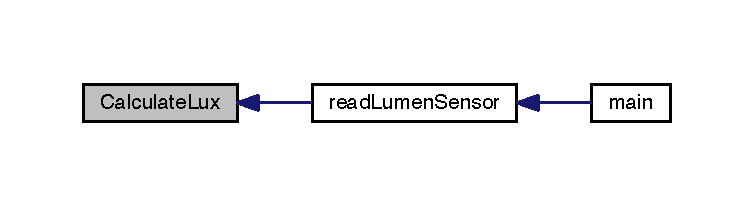
\includegraphics[width=350pt]{de/d08/lux_8c_a3db2aa0d603f0627be256dc108d3d763_icgraph}
\end{center}
\end{figure}



\hypertarget{lux_8h}{}\subsection{lux.\+h filreference}
\label{lux_8h}\index{lux.\+h@{lux.\+h}}


Code copied from the \char`\"{}\+T\+S\+L2561 Light-\/to-\/digital converter\char`\"{} datasheet.  


Denne graf viser, hvilke filer der direkte eller indirekte inkluderer denne fil\+:\nopagebreak
\begin{figure}[H]
\begin{center}
\leavevmode
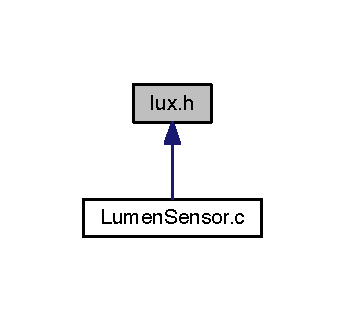
\includegraphics[width=165pt]{df/d85/lux_8h__dep__incl}
\end{center}
\end{figure}
\subsubsection*{Funktioner}
\begin{DoxyCompactItemize}
\item 
unsigned int \hyperlink{lux_8h_a3db2aa0d603f0627be256dc108d3d763}{Calculate\+Lux} (unsigned int i\+Gain, unsigned int t\+Int, unsigned int ch0, unsigned int ch1, int i\+Type)
\begin{DoxyCompactList}\small\item\em Calculate perceived lux from sensor values The sensor has two detectors, one that detects visible and infrared light while the second only detects infrared light. The amount of visible light is then calculated by substracting a scaling fraction of the second detector value from a scaling fraction of the first. \end{DoxyCompactList}\end{DoxyCompactItemize}


\subsubsection{Detaljeret beskrivelse}
Code copied from the \char`\"{}\+T\+S\+L2561 Light-\/to-\/digital converter\char`\"{} datasheet. 

\begin{DoxyAuthor}{Forfatter}
T\+A\+OS, Inc. 
\end{DoxyAuthor}


\subsubsection{Funktions-\/dokumentation}
\index{lux.\+h@{lux.\+h}!Calculate\+Lux@{Calculate\+Lux}}
\index{Calculate\+Lux@{Calculate\+Lux}!lux.\+h@{lux.\+h}}
\paragraph[{\texorpdfstring{Calculate\+Lux(unsigned int i\+Gain, unsigned int t\+Int, unsigned int ch0, unsigned int ch1, int i\+Type)}{CalculateLux(unsigned int iGain, unsigned int tInt, unsigned int ch0, unsigned int ch1, int iType)}}]{\setlength{\rightskip}{0pt plus 5cm}unsigned int Calculate\+Lux (
\begin{DoxyParamCaption}
\item[{unsigned int}]{i\+Gain, }
\item[{unsigned int}]{t\+Int, }
\item[{unsigned int}]{ch0, }
\item[{unsigned int}]{ch1, }
\item[{int}]{i\+Type}
\end{DoxyParamCaption}
)}\hypertarget{lux_8h_a3db2aa0d603f0627be256dc108d3d763}{}\label{lux_8h_a3db2aa0d603f0627be256dc108d3d763}


Calculate perceived lux from sensor values The sensor has two detectors, one that detects visible and infrared light while the second only detects infrared light. The amount of visible light is then calculated by substracting a scaling fraction of the second detector value from a scaling fraction of the first. 

\begin{DoxyReturn}{Returnerer}
The calculated lux value 
\end{DoxyReturn}

\begin{DoxyParams}[1]{Parametre}
\mbox{\tt in}  & {\em i\+Gain} & Is internal scaling enabled in the sensor (0 = x1, 1 = x16) \\
\hline
\mbox{\tt in}  & {\em t\+Int} & Integration time set in the sensor (0 = 13.\+7ms, 1 = 101ms, 2 = 402ms) \\
\hline
\mbox{\tt in}  & {\em ch0} & Value read from detector 0 \\
\hline
\mbox{\tt in}  & {\em ch1} & Value read from detector 1 \\
\hline
\mbox{\tt in}  & {\em i\+Type} & Physical sensor package (0 = T, FN or CL, 1 = CS)\\
\hline
\end{DoxyParams}
\begin{DoxyAuthor}{Forfatter}
T\+A\+OS, Inc. 
\end{DoxyAuthor}


Defineret på linje 147 i filen lux.\+c.



Indeholder referencer til B1C, B1T, B2C, B2T, B3C, B3T, B4C, B4T, B5C, B5T, B6C, B6T, B7C, B7T, B8C, B8T, C\+H\+\_\+\+S\+C\+A\+LE, C\+H\+S\+C\+A\+L\+E\+\_\+\+T\+I\+N\+T0, C\+H\+S\+C\+A\+L\+E\+\_\+\+T\+I\+N\+T1, K1C, K1T, K2C, K2T, K3C, K3T, K4C, K4T, K5C, K5T, K6C, K6T, K7C, K7T, K8C, K8T, L\+U\+X\+\_\+\+S\+C\+A\+LE, M1C, M1T, M2C, M2T, M3C, M3T, M4C, M4T, M5C, M5T, M6C, M6T, M7C, M7T, M8C, M8T og R\+A\+T\+I\+O\+\_\+\+S\+C\+A\+LE.



Refereret til af read\+Lumen\+Sensor().


\begin{DoxyCode}
149 \{
150   \textcolor{comment}{//}
151   \textcolor{comment}{// first, scale the channel values depending on the gain and integration time}
152   \textcolor{comment}{// 16X, 402mS is nominal.}
153   \textcolor{comment}{// scale if integration time is NOT 402 msec}
154   \textcolor{keywordtype}{unsigned} \textcolor{keywordtype}{long} chScale;
155   \textcolor{keywordtype}{unsigned} \textcolor{keywordtype}{long} channel1;
156   \textcolor{keywordtype}{unsigned} \textcolor{keywordtype}{long} channel0;
157   \textcolor{keywordflow}{switch} (tInt)
158   \{
159     \textcolor{keywordflow}{case} 0: \textcolor{comment}{// 13.7 msec}
160       chScale = \hyperlink{lux_8c_af740a064eaa0da3339e7eba683a671ed}{CHSCALE\_TINT0};
161       \textcolor{keywordflow}{break};
162     \textcolor{keywordflow}{case} 1: \textcolor{comment}{// 101 msec}
163       chScale = \hyperlink{lux_8c_a1f741d16494e81486136c73489097cdd}{CHSCALE\_TINT1};
164       \textcolor{keywordflow}{break};
165     \textcolor{keywordflow}{default}: \textcolor{comment}{// assume no scaling}
166       chScale = (1 << \hyperlink{lux_8c_ae77b11d54490369c690da18aef1e76e5}{CH\_SCALE});
167       \textcolor{keywordflow}{break};
168   \}
169   \textcolor{comment}{// scale if gain is NOT 16X}
170   \textcolor{keywordflow}{if} (!iGain) chScale = chScale << 4; \textcolor{comment}{// scale 1X to 16X}
171   \textcolor{comment}{// scale the channel values}
172   channel0 = (ch0 * chScale) >> \hyperlink{lux_8c_ae77b11d54490369c690da18aef1e76e5}{CH\_SCALE};
173   channel1 = (ch1 * chScale) >> \hyperlink{lux_8c_ae77b11d54490369c690da18aef1e76e5}{CH\_SCALE};
174   \textcolor{comment}{//}
175   \textcolor{comment}{// find the ratio of the channel values (Channel1/Channel0)}
176   \textcolor{comment}{// protect against divide by zero}
177   \textcolor{keywordtype}{unsigned} \textcolor{keywordtype}{long} ratio1 = 0;
178   \textcolor{keywordflow}{if} (channel0 != 0) ratio1 = (channel1 << (\hyperlink{lux_8c_a2d36ccf8157f890c015eddd64276d77c}{RATIO\_SCALE}+1)) / channel0;
179   \textcolor{comment}{// round the ratio value}
180   \textcolor{keywordtype}{unsigned} \textcolor{keywordtype}{long} ratio = (ratio1 + 1) >> 1;
181   \textcolor{comment}{// is ratio <= eachBreak ?}
182   \textcolor{keywordtype}{unsigned} \textcolor{keywordtype}{int} b = 0, m = 0;
183   \textcolor{keywordflow}{switch} (iType)
184   \{
185     \textcolor{keywordflow}{case} 0: \textcolor{comment}{// T, FN and CL package}
186       \textcolor{keywordflow}{if} ((ratio >= 0) && (ratio <= \hyperlink{lux_8c_a8d1758888413b06317d05260d023c6f1}{K1T}))
187       \{b=\hyperlink{lux_8c_a77a115660299dfe589547bd1c9313e18}{B1T}; m=\hyperlink{lux_8c_a9cee464de95fd9f1cc41e4737cdfcf56}{M1T};\}
188       \textcolor{keywordflow}{else} \textcolor{keywordflow}{if} (ratio <= \hyperlink{lux_8c_af3f76dac869af6d4fb8834ba8e5baa72}{K2T})
189       \{b=\hyperlink{lux_8c_a0a24c8d38c744a6706fbef06cc0d045e}{B2T}; m=\hyperlink{lux_8c_af13d82736a980dd7f78a0c8633c656c0}{M2T};\}
190       \textcolor{keywordflow}{else} \textcolor{keywordflow}{if} (ratio <= \hyperlink{lux_8c_a96898795c866703216e3035ecc1c29aa}{K3T})
191       \{b=\hyperlink{lux_8c_aa58a8a3b4010f1d8ab947e2351b6cf1d}{B3T}; m=\hyperlink{lux_8c_a6d02cd58020bf44d98927446668a2f7b}{M3T};\}
192       \textcolor{keywordflow}{else} \textcolor{keywordflow}{if} (ratio <= \hyperlink{lux_8c_aa3489bee2d8a1e25002669517f4b6f7d}{K4T})
193       \{b=\hyperlink{lux_8c_a836fd96912939cd386f83e20ed1061ee}{B4T}; m=\hyperlink{lux_8c_ac5983b281c3a2f1d4ea1f87236cfcb44}{M4T};\}
194       \textcolor{keywordflow}{else} \textcolor{keywordflow}{if} (ratio <= \hyperlink{lux_8c_a7df915d6ba425afa9a463f249168d6bd}{K5T})
195       \{b=\hyperlink{lux_8c_a8a3732432706e9a5a5ae3d3485d47043}{B5T}; m=\hyperlink{lux_8c_a2d9fce4a16f258b5ab02b09a954648f6}{M5T};\}
196       \textcolor{keywordflow}{else} \textcolor{keywordflow}{if} (ratio <= \hyperlink{lux_8c_a677e2edf3cf15bef63405c35a7be1310}{K6T})
197       \{b=\hyperlink{lux_8c_ab01465ad82a39e8d02c2dd79279bfe38}{B6T}; m=\hyperlink{lux_8c_a48074a633649636c0748b851a23776df}{M6T};\}
198       \textcolor{keywordflow}{else} \textcolor{keywordflow}{if} (ratio <= \hyperlink{lux_8c_a7e788fd48d058b89ffcc0438bc3d558e}{K7T})
199       \{b=\hyperlink{lux_8c_ad61180572632999584ac8b582a00e2c8}{B7T}; m=\hyperlink{lux_8c_aa3094566ff7a1a2bcd210e256c7b50cc}{M7T};\}
200       \textcolor{keywordflow}{else} \textcolor{keywordflow}{if} (ratio > \hyperlink{lux_8c_aa0dc3961e2039ad7d91faf6829ec1404}{K8T})
201       \{b=\hyperlink{lux_8c_ab5d069e613c69aaf71ea97b129cc5ec1}{B8T}; m=\hyperlink{lux_8c_acb54eadab753bfe327548d7216edd9a2}{M8T};\}
202       \textcolor{keywordflow}{break};
203     \textcolor{keywordflow}{case} 1:\textcolor{comment}{// CS package}
204       \textcolor{keywordflow}{if} ((ratio >= 0) && (ratio <= \hyperlink{lux_8c_a5d91e3222633d82540d7ce0e8d2e1bb2}{K1C}))
205       \{b=\hyperlink{lux_8c_a93aa8f0bb51f43d51e78656a352c6d16}{B1C}; m=\hyperlink{lux_8c_a4ec6175326ca3eb8b731a162b6fcd866}{M1C};\}
206       \textcolor{keywordflow}{else} \textcolor{keywordflow}{if} (ratio <= \hyperlink{lux_8c_ac91e954471045fdbd9b3d01933373c1e}{K2C})
207       \{b=\hyperlink{lux_8c_a95f02da704fdc6c1cabd0c29713cee66}{B2C}; m=\hyperlink{lux_8c_ab70590fa6ebed50a3ab8ff17c22b55b2}{M2C};\}
208       \textcolor{keywordflow}{else} \textcolor{keywordflow}{if} (ratio <= \hyperlink{lux_8c_acbc83f137380f27faf46af997f35f882}{K3C})
209       \{b=\hyperlink{lux_8c_ac03c4526fc8c17d71c8ee2171537facd}{B3C}; m=\hyperlink{lux_8c_a172d826f878378caa7889305ad29011f}{M3C};\}
210       \textcolor{keywordflow}{else} \textcolor{keywordflow}{if} (ratio <= \hyperlink{lux_8c_a2fccbc87358653185282ba16b03a64ee}{K4C})
211       \{b=\hyperlink{lux_8c_a6bd8165e32f19978994245c552b8ee2d}{B4C}; m=\hyperlink{lux_8c_abca79308fb0392b1f8c9d5cfeb5310a0}{M4C};\}
212       \textcolor{keywordflow}{else} \textcolor{keywordflow}{if} (ratio <= \hyperlink{lux_8c_aa39a8eec5ffe9f84c4ac098724c70c91}{K5C})
213       \{b=\hyperlink{lux_8c_af4a1b651ec51bb418ce1bffb87fa79e4}{B5C}; m=\hyperlink{lux_8c_a7c5adce134d8d2be44024c075f55c5c1}{M5C};\}
214       \textcolor{keywordflow}{else} \textcolor{keywordflow}{if} (ratio <= \hyperlink{lux_8c_a9dccc63bcf43c1b4714e913053a906c1}{K6C})
215       \{b=\hyperlink{lux_8c_abe71d8a87f6d974ee3d26693d1a2ea51}{B6C}; m=\hyperlink{lux_8c_a2140b89133d826e76d2a717a3d863551}{M6C};\}
216       \textcolor{keywordflow}{else} \textcolor{keywordflow}{if} (ratio <= \hyperlink{lux_8c_ac104bf3b33df4e42b14dc31078283565}{K7C})
217       \{b=\hyperlink{lux_8c_a5750be8469107d68ea4bdd4e4947316b}{B7C}; m=\hyperlink{lux_8c_acc5b1974656133787900e9bd5219c5ce}{M7C};\}
218       \textcolor{keywordflow}{else} \textcolor{keywordflow}{if} (ratio > \hyperlink{lux_8c_ac47a903b8bc65dc56915024f00201213}{K8C})
219       \{b=\hyperlink{lux_8c_a6d9dfce0cef08b9ef488e582ac4f92e9}{B8C}; m=\hyperlink{lux_8c_ac15c8f99823ed2ff447fb568ce4d3957}{M8C};\}
220       \textcolor{keywordflow}{break};
221   \}
222   \textcolor{keywordtype}{unsigned} \textcolor{keywordtype}{long} temp;
223   temp = ((channel0 * b) - (channel1 * m));
224   \textcolor{comment}{// do not allow negative lux value}
225   \textcolor{keywordflow}{if} (temp < 0) temp = 0;
226   \textcolor{comment}{//}
227   temp += (1 << (\hyperlink{lux_8c_abe3540b1f05e5974dfa40491719b322a}{LUX\_SCALE}-1));
228   \textcolor{comment}{// strip off fractional portion}
229   \textcolor{keywordtype}{unsigned} \textcolor{keywordtype}{long} lux = temp >> \hyperlink{lux_8c_abe3540b1f05e5974dfa40491719b322a}{LUX\_SCALE};
230   \textcolor{keywordflow}{return}(lux);
231 \}
\end{DoxyCode}


Her er kalder-\/grafen for denne funktion\+:\nopagebreak
\begin{figure}[H]
\begin{center}
\leavevmode
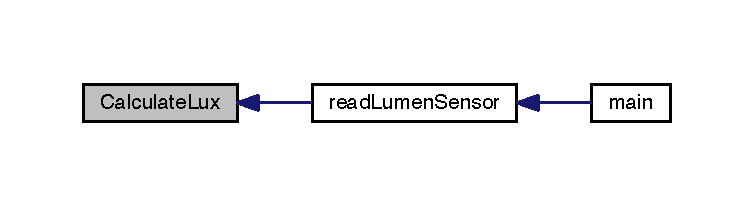
\includegraphics[width=350pt]{d9/dc2/lux_8h_a3db2aa0d603f0627be256dc108d3d763_icgraph}
\end{center}
\end{figure}



\hypertarget{main_8c}{}\subsection{main.\+c filreference}
\label{main_8c}\index{main.\+c@{main.\+c}}


Hovedprogram.  


{\ttfamily \#include $<$project.\+h$>$}\\*
{\ttfamily \#include \char`\"{}data.\+h\char`\"{}}\\*
{\ttfamily \#include \char`\"{}handler.\+h\char`\"{}}\\*
{\ttfamily \#include \char`\"{}i2c.\+h\char`\"{}}\\*
{\ttfamily \#include \char`\"{}led.\+h\char`\"{}}\\*
{\ttfamily \#include \char`\"{}queue.\+h\char`\"{}}\\*
{\ttfamily \#include \char`\"{}xy.\+h\char`\"{}}\\*
Inklusions-\/afhængighedsgraf for main.\+c\+:
\nopagebreak
\begin{figure}[H]
\begin{center}
\leavevmode
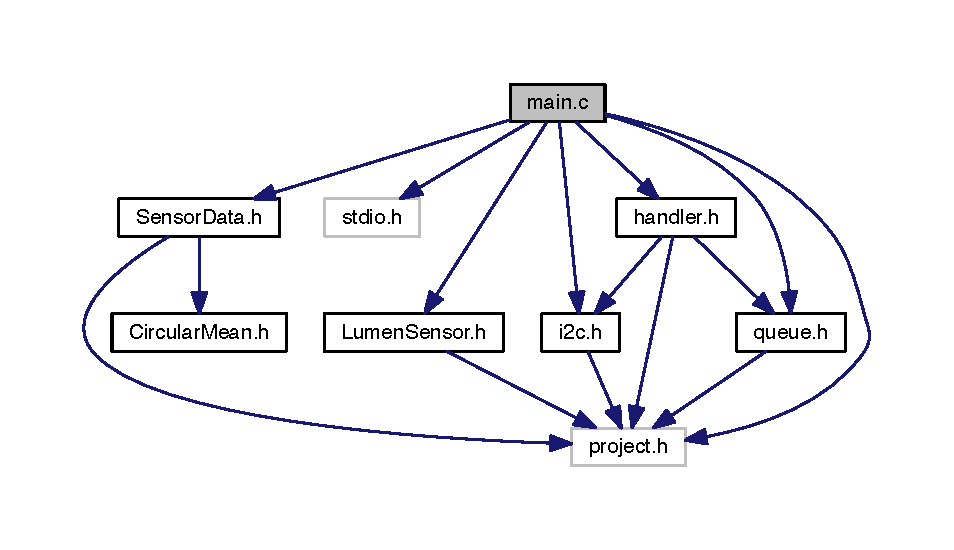
\includegraphics[width=350pt]{d4/d10/main_8c__incl}
\end{center}
\end{figure}
\subsubsection*{Funktioner}
\begin{DoxyCompactItemize}
\item 
int \hyperlink{main_8c_ae66f6b31b5ad750f1fe042a706a4e3d4}{main} ()
\end{DoxyCompactItemize}


\subsubsection{Detaljeret beskrivelse}
Hovedprogram. 

Intilizere modulerne og køre derefter i loop hvor der bliver kontrolieret om der er nogle actions i køen der skal håndteres af handleren. \begin{DoxyAuthor}{Forfatter}
Casper Dieu Le (\href{mailto:201370338@uni.au.dk}{\tt 201370338@uni.\+au.\+dk}) 

Kasper Hinkler Uldbjerg (\href{mailto:201370281@uni.au.dk}{\tt 201370281@uni.\+au.\+dk}) 

Jeppe Stærk (\href{mailto:201271201@uni.au.dk}{\tt 201271201@uni.\+au.\+dk}) 
\end{DoxyAuthor}


\subsubsection{Funktions-\/dokumentation}
\index{main.\+c@{main.\+c}!main@{main}}
\index{main@{main}!main.\+c@{main.\+c}}
\paragraph[{\texorpdfstring{main()}{main()}}]{\setlength{\rightskip}{0pt plus 5cm}int main (
\begin{DoxyParamCaption}
{}
\end{DoxyParamCaption}
)}\hypertarget{main_8c_ae66f6b31b5ad750f1fe042a706a4e3d4}{}\label{main_8c_ae66f6b31b5ad750f1fe042a706a4e3d4}


Defineret på linje 17 i filen main.\+c.



Indeholder referencer til X\+Y\+::calibrate\+X(), X\+Y\+::calibrate\+Y(), Data\+::data\+\_\+init(), Queue\+::front\+Queue(), Handler\+::handler(), I2\+C\+::i2c\+\_\+init(), I2\+C\+::i2c\+\_\+tx(), Queue\+::is\+Empty\+Queue(), Queue\+::pop\+Queue(), Queue\+::queue\+\_\+init(), L\+E\+D\+::set\+Led(), X\+Y\+::xy\+\_\+init() og X\+Y\+::xy\+\_\+start().


\begin{DoxyCode}
18 \{
19   CyGlobalIntEnable;
20   
21   \hyperlink{class_data_adf37c815716edf228a3cbb4564290275}{data\_init}();
22   \hyperlink{class_queue_a4e0a3758d721506e7729f4d074a280ff}{queue\_init}(6u);
23   \hyperlink{class_x_y_aaf6d50e1866014a76b1b15325d2dba4b}{xy\_init}();
24   \hyperlink{class_i2_c_a64303230bf4843297e7ac37ac236ca04}{i2c\_init}();
25   
26   DEBUG\_PutCRLF();
27   DEBUG\_PutString(\textcolor{stringliteral}{"===== Initializing PSoC XY ====="});
28   DEBUG\_PutCRLF();
29   
30   \hyperlink{class_l_e_d_a1d8e725e3829da99c1d027ba0a2ce57a}{setLed}(0,1,0,0);
31   CyDelay(100);
32   \hyperlink{class_l_e_d_a1d8e725e3829da99c1d027ba0a2ce57a}{setLed}(0,0,0,0);
33   
34   \hyperlink{class_x_y_a47c6cc7fae92395e4d1231428c7070d4}{xy\_start}();
35   
36   \textcolor{keywordflow}{for}(;;)
37   \{
38     \textcolor{keywordflow}{if}(SW2\_Read() == 0u)
39     \{
40       CyDelay(5u);
41       \textcolor{keywordflow}{if}(SW2\_Read() == 0u)
42       \{
43         \hyperlink{class_x_y_a852d7d757cec8e85e0b436969d0ce237}{calibrateX}();
44         \hyperlink{class_x_y_a86751f168bdc352fa109644298829609}{calibrateY}();
45       \}
46       \textcolor{keywordflow}{while}(SW2\_Read() == 0u)
47       \{
48         ; \textcolor{comment}{/* Wait till button released */}
49       \}
50     \}
51     
52     \textcolor{keywordflow}{while}(\hyperlink{class_queue_aafb324c79731abdc228dbf94d86722a3}{isEmptyQueue}() != 1)
53     \{
54       \textcolor{keyword}{struct }\hyperlink{queue_8h_df/d8c/struct_action}{Action} action;
55       action = \hyperlink{class_queue_a49c50ba30a42033068d8d8e6a23c6ca1}{frontQueue}();
56       \hyperlink{class_handler_af5be5b016b862943cd22504490acc8f4}{handler}(action.cmd, action.val);
57       \hyperlink{class_queue_a9ecab9ecdedfc331aed9a0ae63ce193b}{popQueue}();
58     \}
59     \hyperlink{class_i2_c_a3d3187ad377a6ca29b3fac5c809b6012}{i2c\_tx}();
60   \}
61 \}
\end{DoxyCode}


Her er kald-\/grafen for denne funktion\+:
\nopagebreak
\begin{figure}[H]
\begin{center}
\leavevmode
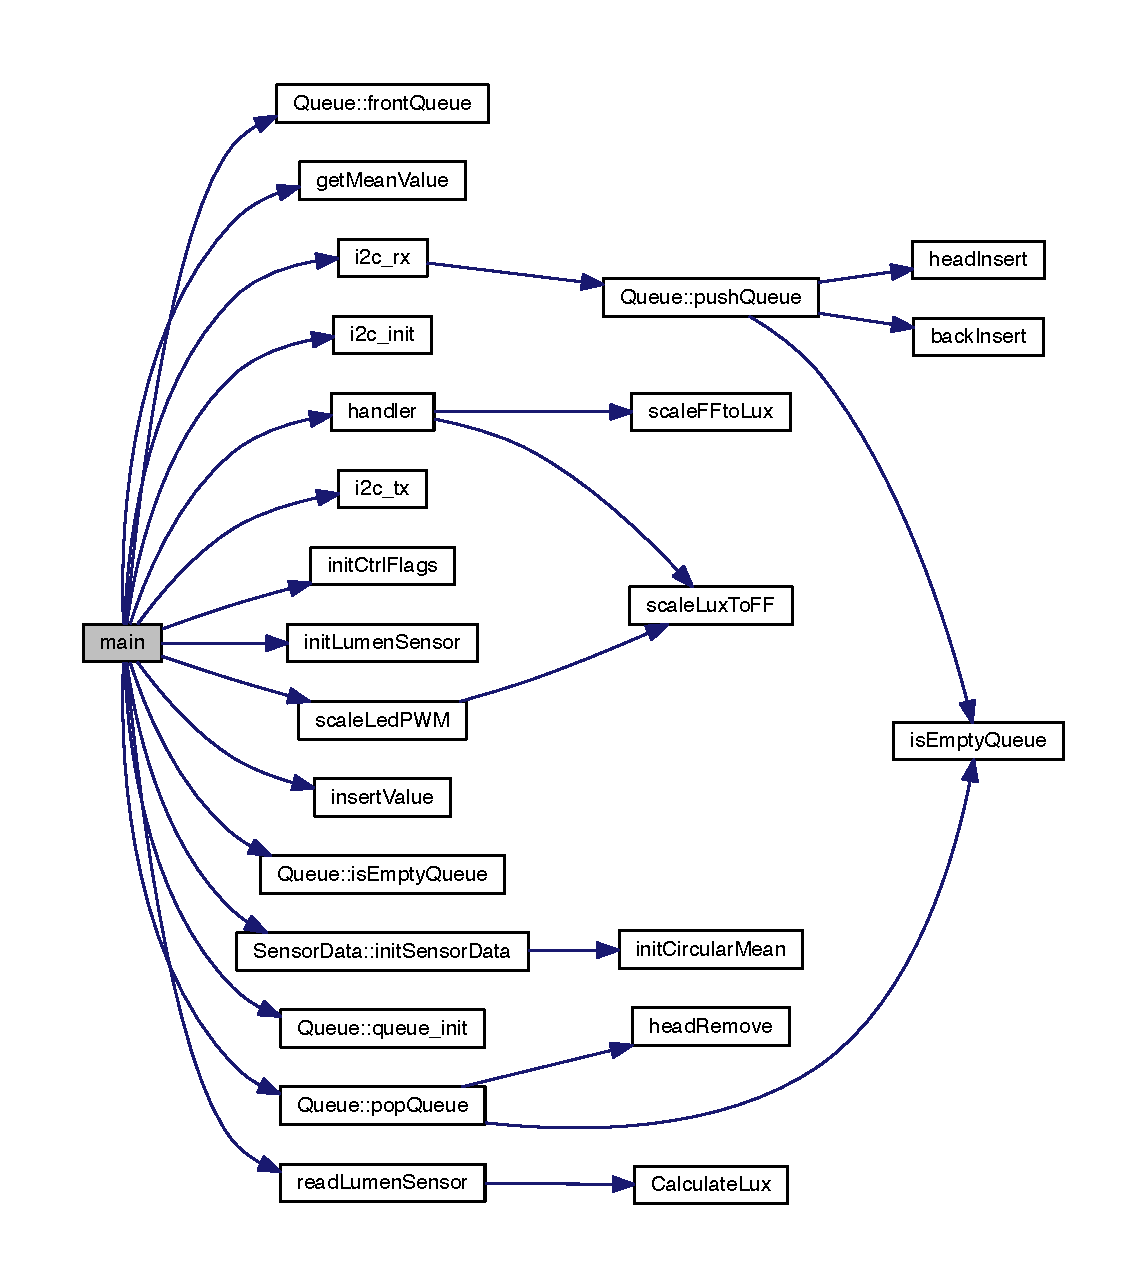
\includegraphics[width=350pt]{d0/d29/main_8c_ae66f6b31b5ad750f1fe042a706a4e3d4_cgraph}
\end{center}
\end{figure}



\hypertarget{queue_8c}{}\subsection{queue.\+c filreference}
\label{queue_8c}\index{queue.\+c@{queue.\+c}}


A queue for incoming commands.  


{\ttfamily \#include \char`\"{}queue.\+h\char`\"{}}\\*
{\ttfamily \#include $<$stdio.\+h$>$}\\*
{\ttfamily \#include $<$stdlib.\+h$>$}\\*
Inklusions-\/afhængighedsgraf for queue.\+c\+:
\nopagebreak
\begin{figure}[H]
\begin{center}
\leavevmode
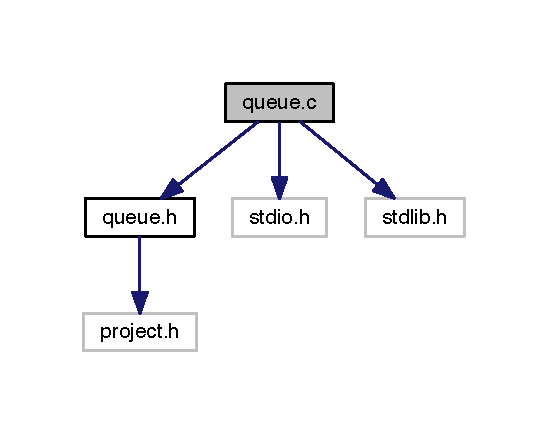
\includegraphics[width=263pt]{d1/d50/queue_8c__incl}
\end{center}
\end{figure}
\subsubsection*{Datastrukturer}
\begin{DoxyCompactItemize}
\item 
struct \hyperlink{queue_8c_db/d8b/struct_node}{Node}
\begin{DoxyCompactList}\small\item\em Struct to contain a element in the queue.  \hyperlink{queue_8c_db/d8b/struct_node}{Mere...}\end{DoxyCompactList}\end{DoxyCompactItemize}
\subsubsection*{Funktioner}
\begin{DoxyCompactItemize}
\item 
static void \hyperlink{queue_8c_a2607abf0fdd9192a8da3b72245bf593f}{head\+Insert} (struct \hyperlink{queue_8c_db/d8b/struct_node}{Node} $\ast$$\ast$head\+Ptr, const struct \hyperlink{queue_8h_da/d48/struct_data}{Data} data)
\item 
static void \hyperlink{queue_8c_a3f4e77137b39d4f0461d240a5a372917}{head\+Remove} (struct \hyperlink{queue_8c_db/d8b/struct_node}{Node} $\ast$$\ast$head\+Ptr)
\item 
static void \hyperlink{queue_8c_a8e59eeb600ef9f52372bfcb13d1fb6ff}{back\+Insert} (struct \hyperlink{queue_8c_db/d8b/struct_node}{Node} $\ast$$\ast$back\+Ptr, const struct \hyperlink{queue_8h_da/d48/struct_data}{Data} data)
\end{DoxyCompactItemize}


\subsubsection{Detaljeret beskrivelse}
A queue for incoming commands. 



\subsubsection{Datastruktur-\/documentation}
\index{Node@{Node}}\label{struct_node}
\hypertarget{queue_8c_struct_node}{}
\paragraph{struct Node}
Struct to contain a element in the queue. 

\begin{DoxyAuthor}{Forfatter}
Jeppe Stærk (\href{mailto:201271201@uni.au.dk}{\tt 201271201@uni.\+au.\+dk}) 
\end{DoxyAuthor}


Defineret på linje 20 i filen queue.\+c.



Samarbejdsdiagram for Node\+:
\nopagebreak
\begin{figure}[H]
\begin{center}
\leavevmode
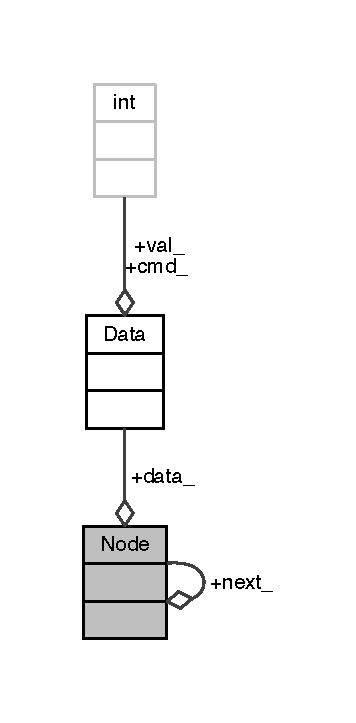
\includegraphics[width=171pt]{df/ddc/struct_node__coll__graph}
\end{center}
\end{figure}
\begin{DoxyFields}{Data-\/felter}
struct \hyperlink{queue_8h_da/d48/struct_data}{Data}\hypertarget{queue_8c_ab6f992d78ad6bf73e17978ce064d0546}{}\label{queue_8c_ab6f992d78ad6bf73e17978ce064d0546}
&
data\+\_\+&
\hyperlink{queue_8h_da/d48/struct_data}{Data} stored in queue \\
\hline

struct \hyperlink{queue_8c_db/d8b/struct_node}{Node} $\ast$\hypertarget{queue_8c_a882bca6dea645e11ca1df6bc3c30ac42}{}\label{queue_8c_a882bca6dea645e11ca1df6bc3c30ac42}
&
next\+\_\+&
Next node in queue \\
\hline

\end{DoxyFields}


\subsubsection{Funktions-\/dokumentation}
\index{queue.\+c@{queue.\+c}!back\+Insert@{back\+Insert}}
\index{back\+Insert@{back\+Insert}!queue.\+c@{queue.\+c}}
\paragraph[{\texorpdfstring{back\+Insert(struct Node $\ast$$\ast$back\+Ptr, const struct Data data)}{backInsert(struct Node **backPtr, const struct Data data)}}]{\setlength{\rightskip}{0pt plus 5cm}static void back\+Insert (
\begin{DoxyParamCaption}
\item[{struct {\bf Node} $\ast$$\ast$}]{back\+Ptr, }
\item[{const struct {\bf Data}}]{data}
\end{DoxyParamCaption}
)\hspace{0.3cm}{\ttfamily [static]}}\hypertarget{queue_8c_a8e59eeb600ef9f52372bfcb13d1fb6ff}{}\label{queue_8c_a8e59eeb600ef9f52372bfcb13d1fb6ff}


Refereret til af Queue\+::push\+Queue().



Her er kalder-\/grafen for denne funktion\+:
\nopagebreak
\begin{figure}[H]
\begin{center}
\leavevmode
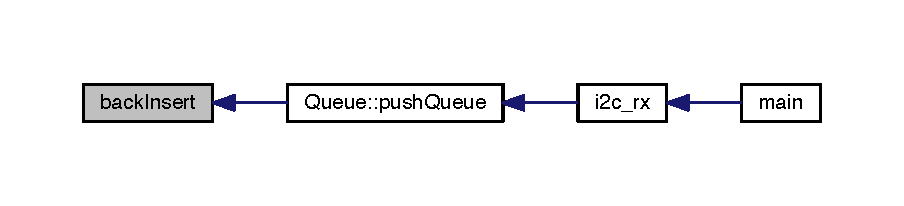
\includegraphics[width=350pt]{d2/dbd/queue_8c_a8e59eeb600ef9f52372bfcb13d1fb6ff_icgraph}
\end{center}
\end{figure}


\index{queue.\+c@{queue.\+c}!head\+Insert@{head\+Insert}}
\index{head\+Insert@{head\+Insert}!queue.\+c@{queue.\+c}}
\paragraph[{\texorpdfstring{head\+Insert(struct Node $\ast$$\ast$head\+Ptr, const struct Data data)}{headInsert(struct Node **headPtr, const struct Data data)}}]{\setlength{\rightskip}{0pt plus 5cm}static void head\+Insert (
\begin{DoxyParamCaption}
\item[{struct {\bf Node} $\ast$$\ast$}]{head\+Ptr, }
\item[{const struct {\bf Data}}]{data}
\end{DoxyParamCaption}
)\hspace{0.3cm}{\ttfamily [static]}}\hypertarget{queue_8c_a2607abf0fdd9192a8da3b72245bf593f}{}\label{queue_8c_a2607abf0fdd9192a8da3b72245bf593f}


Refereret til af Queue\+::push\+Queue().



Her er kalder-\/grafen for denne funktion\+:
\nopagebreak
\begin{figure}[H]
\begin{center}
\leavevmode
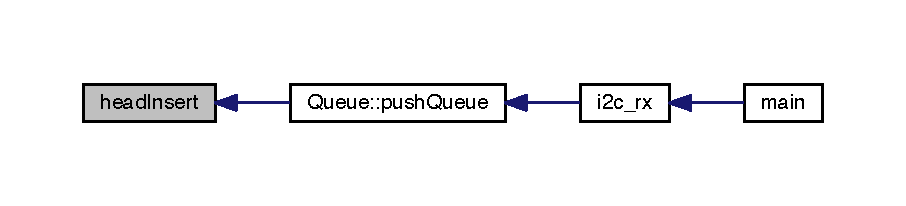
\includegraphics[width=350pt]{d2/dbd/queue_8c_a2607abf0fdd9192a8da3b72245bf593f_icgraph}
\end{center}
\end{figure}


\index{queue.\+c@{queue.\+c}!head\+Remove@{head\+Remove}}
\index{head\+Remove@{head\+Remove}!queue.\+c@{queue.\+c}}
\paragraph[{\texorpdfstring{head\+Remove(struct Node $\ast$$\ast$head\+Ptr)}{headRemove(struct Node **headPtr)}}]{\setlength{\rightskip}{0pt plus 5cm}static void head\+Remove (
\begin{DoxyParamCaption}
\item[{struct {\bf Node} $\ast$$\ast$}]{head\+Ptr}
\end{DoxyParamCaption}
)\hspace{0.3cm}{\ttfamily [static]}}\hypertarget{queue_8c_a3f4e77137b39d4f0461d240a5a372917}{}\label{queue_8c_a3f4e77137b39d4f0461d240a5a372917}


Refereret til af Queue\+::pop\+Queue().



Her er kalder-\/grafen for denne funktion\+:
\nopagebreak
\begin{figure}[H]
\begin{center}
\leavevmode
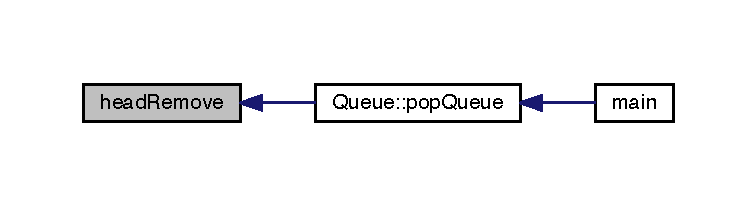
\includegraphics[width=350pt]{d2/dbd/queue_8c_a3f4e77137b39d4f0461d240a5a372917_icgraph}
\end{center}
\end{figure}



\hypertarget{queue_8h}{}\subsection{queue.\+h filreference}
\label{queue_8h}\index{queue.\+h@{queue.\+h}}


A queue for incoming commands.  


{\ttfamily \#include $<$project.\+h$>$}\\*
Inklusions-\/afhængighedsgraf for queue.\+h\+:
\nopagebreak
\begin{figure}[H]
\begin{center}
\leavevmode
\includegraphics[width=134pt]{d9/dc8/queue_8h__incl}
\end{center}
\end{figure}
Denne graf viser, hvilke filer der direkte eller indirekte inkluderer denne fil\+:
\nopagebreak
\begin{figure}[H]
\begin{center}
\leavevmode
\includegraphics[width=311pt]{d2/d5f/queue_8h__dep__incl}
\end{center}
\end{figure}
\subsubsection*{Datastrukturer}
\begin{DoxyCompactItemize}
\item 
struct \hyperlink{queue_8h_da/d48/struct_data}{Data}
\begin{DoxyCompactList}\small\item\em Struct to contain a command and value.  \hyperlink{queue_8h_da/d48/struct_data}{Mere...}\end{DoxyCompactList}\end{DoxyCompactItemize}
\subsubsection*{Funktioner}
\begin{DoxyCompactItemize}
\item 
void \hyperlink{queue_8h_a2f53f032b89a2e6f1906a3d7aef99df3}{queue\+\_\+init} (uint8 queue\+Size)
\item 
void \hyperlink{queue_8h_a0a8b5d336192563403043ec13ab653db}{push\+Queue} (const struct \hyperlink{queue_8h_da/d48/struct_data}{Data} data)
\item 
void \hyperlink{queue_8h_ac6b21d6c7e519088b5ef6d2fcbd56d05}{pop\+Queue} (void)
\item 
struct \hyperlink{queue_8h_da/d48/struct_data}{Data} \hyperlink{queue_8h_af36c0dba474afad4b82dc9a070157ca1}{front\+Queue} (void)
\item 
int \hyperlink{queue_8h_a1ff400b19762977cf8f5cec81c57eace}{is\+Empty\+Queue} (void)
\end{DoxyCompactItemize}
\subsubsection*{Variable}
\begin{DoxyCompactItemize}
\item 
uint8 \hyperlink{queue_8h_ad260f9ccca00e80d161bbf3e70c3ffa6}{queue\+Count\+\_\+}
\end{DoxyCompactItemize}


\subsubsection{Detaljeret beskrivelse}
A queue for incoming commands. 

\begin{DoxyAuthor}{Forfatter}
Jeppe Stærk (\href{mailto:201271201@uni.au.dk}{\tt 201271201@uni.\+au.\+dk}) 
\end{DoxyAuthor}


\subsubsection{Datastruktur-\/documentation}
\index{Data@{Data}}\label{struct_data}
\hypertarget{queue_8h_struct_data}{}
\paragraph{struct Data}
Struct to contain a command and value. 

\begin{DoxyAuthor}{Forfatter}
Jeppe Stærk (\href{mailto:201271201@uni.au.dk}{\tt 201271201@uni.\+au.\+dk}) 
\end{DoxyAuthor}


Defineret på linje 24 i filen queue.\+h.



Samarbejdsdiagram for Data\+:
\nopagebreak
\begin{figure}[H]
\begin{center}
\leavevmode
\includegraphics[width=129pt]{de/d65/struct_data__coll__graph}
\end{center}
\end{figure}
\begin{DoxyFields}{Data-\/felter}
int\hypertarget{queue_8h_a9e053ea62d7d38fa0123be2d16a4f37f}{}\label{queue_8h_a9e053ea62d7d38fa0123be2d16a4f37f}
&
cmd\+\_\+&
Command stored in queue \\
\hline

int\hypertarget{queue_8h_a937c383ba2dbf3514176a2651b61a269}{}\label{queue_8h_a937c383ba2dbf3514176a2651b61a269}
&
val\+\_\+&
Value stored in queue \\
\hline

\end{DoxyFields}


\subsubsection{Funktions-\/dokumentation}
\index{queue.\+h@{queue.\+h}!front\+Queue@{front\+Queue}}
\index{front\+Queue@{front\+Queue}!queue.\+h@{queue.\+h}}
\paragraph[{\texorpdfstring{front\+Queue(void)}{frontQueue(void)}}]{\setlength{\rightskip}{0pt plus 5cm}struct {\bf Data} front\+Queue (
\begin{DoxyParamCaption}
\item[{void}]{}
\end{DoxyParamCaption}
)}\hypertarget{queue_8h_af36c0dba474afad4b82dc9a070157ca1}{}\label{queue_8h_af36c0dba474afad4b82dc9a070157ca1}
\index{queue.\+h@{queue.\+h}!is\+Empty\+Queue@{is\+Empty\+Queue}}
\index{is\+Empty\+Queue@{is\+Empty\+Queue}!queue.\+h@{queue.\+h}}
\paragraph[{\texorpdfstring{is\+Empty\+Queue(void)}{isEmptyQueue(void)}}]{\setlength{\rightskip}{0pt plus 5cm}int is\+Empty\+Queue (
\begin{DoxyParamCaption}
\item[{void}]{}
\end{DoxyParamCaption}
)}\hypertarget{queue_8h_a1ff400b19762977cf8f5cec81c57eace}{}\label{queue_8h_a1ff400b19762977cf8f5cec81c57eace}


Refereret til af Queue\+::pop\+Queue() og Queue\+::push\+Queue().



Her er kalder-\/grafen for denne funktion\+:
\nopagebreak
\begin{figure}[H]
\begin{center}
\leavevmode
\includegraphics[width=350pt]{d8/d38/queue_8h_a1ff400b19762977cf8f5cec81c57eace_icgraph}
\end{center}
\end{figure}


\index{queue.\+h@{queue.\+h}!pop\+Queue@{pop\+Queue}}
\index{pop\+Queue@{pop\+Queue}!queue.\+h@{queue.\+h}}
\paragraph[{\texorpdfstring{pop\+Queue(void)}{popQueue(void)}}]{\setlength{\rightskip}{0pt plus 5cm}void pop\+Queue (
\begin{DoxyParamCaption}
\item[{void}]{}
\end{DoxyParamCaption}
)}\hypertarget{queue_8h_ac6b21d6c7e519088b5ef6d2fcbd56d05}{}\label{queue_8h_ac6b21d6c7e519088b5ef6d2fcbd56d05}
\index{queue.\+h@{queue.\+h}!push\+Queue@{push\+Queue}}
\index{push\+Queue@{push\+Queue}!queue.\+h@{queue.\+h}}
\paragraph[{\texorpdfstring{push\+Queue(const struct Data data)}{pushQueue(const struct Data data)}}]{\setlength{\rightskip}{0pt plus 5cm}void push\+Queue (
\begin{DoxyParamCaption}
\item[{const struct {\bf Data}}]{data}
\end{DoxyParamCaption}
)}\hypertarget{queue_8h_a0a8b5d336192563403043ec13ab653db}{}\label{queue_8h_a0a8b5d336192563403043ec13ab653db}
\index{queue.\+h@{queue.\+h}!queue\+\_\+init@{queue\+\_\+init}}
\index{queue\+\_\+init@{queue\+\_\+init}!queue.\+h@{queue.\+h}}
\paragraph[{\texorpdfstring{queue\+\_\+init(uint8 queue\+Size)}{queue_init(uint8 queueSize)}}]{\setlength{\rightskip}{0pt plus 5cm}void queue\+\_\+init (
\begin{DoxyParamCaption}
\item[{uint8}]{queue\+Size}
\end{DoxyParamCaption}
)}\hypertarget{queue_8h_a2f53f032b89a2e6f1906a3d7aef99df3}{}\label{queue_8h_a2f53f032b89a2e6f1906a3d7aef99df3}


\subsubsection{Variabel-\/dokumentation}
\index{queue.\+h@{queue.\+h}!queue\+Count\+\_\+@{queue\+Count\+\_\+}}
\index{queue\+Count\+\_\+@{queue\+Count\+\_\+}!queue.\+h@{queue.\+h}}
\paragraph[{\texorpdfstring{queue\+Count\+\_\+}{queueCount_}}]{\setlength{\rightskip}{0pt plus 5cm}uint8 queue\+Count\+\_\+}\hypertarget{queue_8h_ad260f9ccca00e80d161bbf3e70c3ffa6}{}\label{queue_8h_ad260f9ccca00e80d161bbf3e70c3ffa6}


Refereret til af Queue\+::pop\+Queue(), Queue\+::push\+Queue() og Queue\+::queue\+\_\+init().


\hypertarget{_sensor_data_8c}{}\subsection{Sensor\+Data.\+c filreference}
\label{_sensor_data_8c}\index{Sensor\+Data.\+c@{Sensor\+Data.\+c}}


Container for sensor data.  


{\ttfamily \#include \char`\"{}Sensor\+Data.\+h\char`\"{}}\\*
Inklusions-\/afhængighedsgraf for Sensor\+Data.\+c\+:\nopagebreak
\begin{figure}[H]
\begin{center}
\leavevmode
\includegraphics[width=236pt]{d4/d5d/_sensor_data_8c__incl}
\end{center}
\end{figure}


\subsubsection{Detaljeret beskrivelse}
Container for sensor data. 

\begin{DoxyAuthor}{Forfatter}
Simon Nejmann (\href{mailto:19981127@uni.au.dk}{\tt 19981127@uni.\+au.\+dk})
\end{DoxyAuthor}

\hypertarget{_sensor_data_8h}{}\subsection{Sensor\+Data.\+h filreference}
\label{_sensor_data_8h}\index{Sensor\+Data.\+h@{Sensor\+Data.\+h}}
{\ttfamily \#include $<$project.\+h$>$}\\*
{\ttfamily \#include \char`\"{}Circular\+Mean.\+h\char`\"{}}\\*
Inklusions-\/afhængighedsgraf for Sensor\+Data.\+h\+:
\nopagebreak
\begin{figure}[H]
\begin{center}
\leavevmode
\includegraphics[width=236pt]{da/daa/_sensor_data_8h__incl}
\end{center}
\end{figure}
Denne graf viser, hvilke filer der direkte eller indirekte inkluderer denne fil\+:
\nopagebreak
\begin{figure}[H]
\begin{center}
\leavevmode
\includegraphics[width=350pt]{d7/d8f/_sensor_data_8h__dep__incl}
\end{center}
\end{figure}
\subsubsection*{Datastrukturer}
\begin{DoxyCompactItemize}
\item 
struct \hyperlink{_sensor_data_8h_d4/d49/structsensor_data_t}{sensor\+DataT}
\begin{DoxyCompactList}\small\item\em Container for sensor data.  \hyperlink{_sensor_data_8h_d4/d49/structsensor_data_t}{Mere...}\end{DoxyCompactList}\end{DoxyCompactItemize}
\subsubsection*{Variable}
\begin{DoxyCompactItemize}
\item 
struct \hyperlink{_sensor_data_8h_d4/d49/structsensor_data_t}{sensor\+DataT} \hyperlink{_sensor_data_8h_a166db779eaca1ca69d6d63aa4fc36674}{sensor\+Data}
\end{DoxyCompactItemize}


\subsubsection{Datastruktur-\/documentation}
\index{sensor\+DataT@{sensor\+DataT}}\label{structsensor_data_t}
\hypertarget{_sensor_data_8h_structsensor_data_t}{}
\paragraph{struct sensor\+DataT}
Container for sensor data. 

Defineret på linje 16 i filen Sensor\+Data.\+h.



Samarbejdsdiagram for sensor\+DataT\+:
\nopagebreak
\begin{figure}[H]
\begin{center}
\leavevmode
\includegraphics[width=350pt]{dc/d44/structsensor_data_t__coll__graph}
\end{center}
\end{figure}
\begin{DoxyFields}{Data-\/felter}
uint8\hypertarget{_sensor_data_8h_ac79167c0eef257a67503f9fbce9d377c}{}\label{_sensor_data_8h_ac79167c0eef257a67503f9fbce9d377c}
&
blue\+P\+W\+M\+Pct&
Power level of the blue L\+ED\+: Scale 0-\/255. \\
\hline

unsigned int\hypertarget{_sensor_data_8h_ad85f2cca5ef7520f1dc87fc48fc6d8e6}{}\label{_sensor_data_8h_ad85f2cca5ef7520f1dc87fc48fc6d8e6}
&
desired\+Lux&
The lux value the system should try to maintain \\
\hline

int\hypertarget{_sensor_data_8h_a477d7465dc8c397bdb795593df890d8b}{}\label{_sensor_data_8h_a477d7465dc8c397bdb795593df890d8b}
&
desired\+Time\+Distance&
The distance the lamp should not be lowered below. Stored in micro-\/seconds for greater resolution \\
\hline

int\hypertarget{_sensor_data_8h_afb9412686cd344ad61757c1c19ba8a87}{}\label{_sensor_data_8h_afb9412686cd344ad61757c1c19ba8a87}
&
distance&
The latest reading from the ultrasonic distance sensor \\
\hline

uint8\hypertarget{_sensor_data_8h_ac83b8257127d55e998596d703ff141ac}{}\label{_sensor_data_8h_ac83b8257127d55e998596d703ff141ac}
&
green\+P\+W\+M\+Pct&
Power level of the green L\+ED\+: Scale 0-\/255. \\
\hline

uint8\hypertarget{_sensor_data_8h_a3fc7bb7b6b9d39b2a6ae384d15fc5b9d}{}\label{_sensor_data_8h_a3fc7bb7b6b9d39b2a6ae384d15fc5b9d}
&
led\+Power&
Are the L\+E\+Ds currently on or off \\
\hline

struct \hyperlink{_circular_mean_8h_d2/ddd/struct_circular_mean}{Circular\+Mean}\hypertarget{_sensor_data_8h_a2ff5a38714ef318f86285c7d8fe4c8ea}{}\label{_sensor_data_8h_a2ff5a38714ef318f86285c7d8fe4c8ea}
&
Lumen\+Mean&
Circular structure. Can add values and get their average. Used for lux measurements \\
\hline

unsigned int\hypertarget{_sensor_data_8h_aeb23f0cb9c43c48bf83c1d75a5c179a4}{}\label{_sensor_data_8h_aeb23f0cb9c43c48bf83c1d75a5c179a4}
&
lux&
The average value of lux measured \\
\hline

uint8\hypertarget{_sensor_data_8h_a8699b179d899b8419f6db53fab22f6cc}{}\label{_sensor_data_8h_a8699b179d899b8419f6db53fab22f6cc}
&
movement&
The latest reading from the P\+IR movement sensor \\
\hline

uint8\hypertarget{_sensor_data_8h_a722c0f415211bda0d848dd8edac4f1fe}{}\label{_sensor_data_8h_a722c0f415211bda0d848dd8edac4f1fe}
&
movement\+Alert\+On&
Should the system react to movement or ignore it \\
\hline

uint8\hypertarget{_sensor_data_8h_a6ac22d5f267938f95b2261ffa3d5e2d2}{}\label{_sensor_data_8h_a6ac22d5f267938f95b2261ffa3d5e2d2}
&
red\+P\+W\+M\+Pct&
Power level of the red L\+ED\+: Scale 0-\/255. \\
\hline

\end{DoxyFields}


\subsubsection{Variabel-\/dokumentation}
\index{Sensor\+Data.\+h@{Sensor\+Data.\+h}!sensor\+Data@{sensor\+Data}}
\index{sensor\+Data@{sensor\+Data}!Sensor\+Data.\+h@{Sensor\+Data.\+h}}
\paragraph[{\texorpdfstring{sensor\+Data}{sensorData}}]{\setlength{\rightskip}{0pt plus 5cm}struct {\bf sensor\+DataT}  sensor\+Data}\hypertarget{_sensor_data_8h_a166db779eaca1ca69d6d63aa4fc36674}{}\label{_sensor_data_8h_a166db779eaca1ca69d6d63aa4fc36674}


Refereret til af C\+Y\+\_\+\+I\+S\+R(), handler(), Sensor\+Data\+::init\+Sensor\+Data(), main() og scale\+Led\+P\+W\+M().


%--- End generated contents ---

% Index
\newpage
\phantomsection
\clearemptydoublepage
\addcontentsline{toc}{section}{Indeks}
\printindex

\end{document}
